%%%  کلاس AUTthesis، نسخه آبان 1397
%%%   دانشگاه صنعتی امیرکبیر                 http://www.aut.ac.ir
%%%  تالار گفتگوی پارسی‌لاتک،       http://forum.parsilatex.com
%%%   آپدیت شده در آبان 95
%%%   پشتیبانی و راهنمایی          badali_farhad@yahoo.com
%%%
%%%   بازبینی و اصلاح شده در آبان ماه 1397
%%%  Tested via TeXstudio in TeXlive 2014-2018.
%%%

%-----------------------------------------------------------------------------------------------------
%        روش اجرا.: 2 بار F1 ، 2 بار  F11(به منظور تولید مراجع) ، دوبار Ctrl+Alt+I (به منظور تولید نمایه) و دو بار F1 -------> مشاهده Pdf
%%%%%%%%%%%%%%%%%%%%%%%%%%%%%%%%%%%%%%%%%%%%%%%%%%%%%%
%   TeXstudio as your IDE
%%  برای compile در TeXstudio تنها کافی است منوی Options->Configure TeXstudio را زده و در پنجره Configure TeXstudio در بخش Build گزینه Default Compiler را به XeLaTeX تغییر دهید. سند شما به راحتی compile خواهد شد.
%   F1 & F5 : Build & view
%   F6      : Compile
%   F7      : View
%   --------------
%%%%%%%%%%%%%%%%%%%%%%%%%%%%%%%%%%%%%%%%%%%%%%%%%%%%%%
%        اگر قصد نوشتن رساله دکتری را دارید، در خط زیر به جای msc،
%      کلمه phd را قرار دهید. کلیه تنظیمات لازم، به طور خودکار، اعمال می‌شود.
%%% !TEX TS-program = XeLaTeX
\documentclass[oneside,bsc,12pt]{AUTthesis}
%       فایل commands.tex را حتماً به دقت مطالعه کنید؛ چون دستورات مربوط به فراخوانی بسته زی‌پرشین 
%       و دیگر بسته‌ها و ... در این فایل قرار دارد و بهتر است که با نحوه استفاده از آنها آشنا شوید. توجه شود برای نسخه نهایی پایان‌نامه حتماً hyperref را 
%        غیرفعال کنید.


% در این فایل، دستورها و تنظیمات مورد نیاز، آورده شده است.
%-------------------------------------------------------------------------------------------------------------------
% در ورژن جدید زی‌پرشین برای تایپ متن‌های ریاضی، این سه بسته، حتماً باید فراخوانی شود.
\usepackage{amsthm,amssymb,amsmath,amsfonts}
% بسته‌ای برای تنطیم حاشیه‌های بالا، پایین، چپ و راست صفحه
\usepackage[top=30mm, bottom=30mm, left=25mm, right=30mm]{geometry}
% بسته‌‌ای برای ظاهر شدن شکل‌ها و تصاویر متن
\usepackage{graphicx}
\usepackage{color}
%بسته‌ای برای تنظیم فاصله عمودی خط‌های متن
\usepackage{setspace}
\usepackage{titletoc}
\usepackage{tocloft}
%با فعال کردن بسته زیر فوت‌نوت‌ها در هر صفحه ریست می‌شوند. حالت پیش‌فرض آن ریست شدن در هر فصل می‌باشد.
%\usepackage[perpage]{footmisc}
\usepackage{enumitem}
%\usepackage{titlesec}
% بسته‌ و دستوراتی برای ایجاد لینک‌های رنگی با امکان جهش
%\usepackage[pagebackref=false,colorlinks,linkcolor=blue,citecolor=red]{hyperref}
%\usepackage[nameinlink]{cleveref}%capitalize,,noabbrev
% \AtBeginDocument{%
%    \crefname{equation}{برابری}{equations}%
%    \crefname{chapter}{فصل}{chapters}%
%    \crefname{section}{بخش}{sections}%
%    \crefname{appendix}{پیوست}{appendices}%
%    \crefname{enumi}{مورد}{items}%
%    \crefname{footnote}{زیرنویس}{footnotes}%
%    \crefname{figure}{شکل}{figures}%
%    \crefname{table}{جدول}{tables}%
%    \crefname{theorem}{قضیه}{theorems}%
%    \crefname{lemma}{لم}{lemmas}%
%    \crefname{corollary}{نتیجه}{corollaries}%
%    \crefname{proposition}{گزاره}{propositions}%
%    \crefname{definition}{تعریف}{definitions}%
%    \crefname{result}{نتیجه}{results}%
%    \crefname{example}{مثال}{examples}%
%    \crefname{remark}{نکته}{remarks}%
%    \crefname{note}{یادداشت}{notes}%
%}
% چنانچه قصد پرینت گرفتن نوشته خود را دارید، خط بالا را غیرفعال و  از دستور زیر استفاده کنید چون در صورت استفاده از دستور زیر‌‌، 
% لینک‌ها به رنگ سیاه ظاهر خواهند شد که برای پرینت گرفتن، مناسب‌تر است
\usepackage{hyperref}
\usepackage[dvipsnames]{xcolor}
\hypersetup{
	colorlinks=true,
	citecolor=Blue,
	linkcolor=Blue,
	urlcolor=Blue
}
% بسته‌ لازم برای تنظیم سربرگ‌ها
\usepackage{fancyhdr}
% بسته‌ای برای ظاهر شدن «مراجع»  در فهرست مطالب
\usepackage[nottoc]{tocbibind}
% دستورات مربوط به ایجاد نمایه
\usepackage{makeidx,multicol}
\setlength{\columnsep}{1.5cm}

%%%%%%%%%%%%%%%%%%%%%%%%%%
\usepackage{multirow}
\usepackage{ragged2e}
\usepackage[round]{natbib}
\usepackage{caption}
\usepackage{subcaption, array}
\graphicspath{{images/}}
\newcolumntype{P}[1]{>{\centering\arraybackslash}p{#1}}
\newcolumntype{M}[1]{>{\centering\arraybackslash}m{#1}}

\usepackage{verbatim}
\makeindex
\usepackage{sectsty}
% فراخوانی بسته زی‌پرشین و تعریف قلم فارسی و انگلیسی
\usepackage{xepersian}%[extrafootnotefeatures]
\SepMark{-}
%حتماً از تک لایو 2014 استفاده کنید.
\settextfont[Scale=1.2]{B Nazanin}
\setlatintextfont{Times New Roman}
\renewcommand{\labelitemi}{$\bullet$}
%%%%%%%%%%%%%%%%%%%%%%%%%%
% چنانچه می‌خواهید اعداد در فرمول‌ها، انگلیسی باشد، خط زیر را غیرفعال کنید.
%در غیر اینصورت حتماً فونت PGaramond را نصب کنید.
\setdigitfont[Scale=1.1]{PGaramond}%%Yas
%%%%%%%%%%%%%%%%%%%%%%%%%%
% تعریف قلم‌های فارسی اضافی برای استفاده در بعضی از قسمت‌های متن
\defpersianfont\nastaliq[Scale=2]{IranNastaliq}
\defpersianfont\chapternumber[Scale=3]{B Nazanin}
%\chapterfont{\centering}%
%%%%%%%%%%%%%%%%%%%%%%%%%%
% دستوری برای تغییر نام کلمه «اثبات» به «برهان»
\renewcommand\proofname{\textbf{برهان}}

% دستوری برای تغییر نام کلمه «کتاب‌نامه» به «منابع و مراجع«
\renewcommand{\bibname}{منابع و مراجع}


% Headings for every page of ToC, LoF and Lot
\setlength{\cftbeforetoctitleskip}{-1.2em}
\setlength{\cftbeforelottitleskip}{-1.2em}
\setlength{\cftbeforeloftitleskip}{-1.2em}
\setlength{\cftaftertoctitleskip}{-1em}
\setlength{\cftafterlottitleskip}{-1em}
\setlength{\cftafterloftitleskip}{-1em}
%%\makeatletter
%%%%\renewcommand{\l@chapter}{\@dottedtocline{1}{1em\bfseries}{1em}}
%%%%\renewcommand{\l@section}{\@dottedtocline{2}{2em}{2em}}
%%%%\renewcommand{\l@subsection}{\@dottedtocline{3}{3em}{3em}}
%%%%\renewcommand{\l@subsubsection}{\@dottedtocline{4}{4em}{4em}}
%%%%\makeatother


\newcommand\tocheading{\par عنوان\hfill صفحه \par}
\newcommand\lofheading{\hspace*{.5cm}\figurename\hfill صفحه \par}
\newcommand\lotheading{\hspace*{.5cm}\tablename\hfill صفحه \par}

\renewcommand{\cftchapleader}{\cftdotfill{\cftdotsep}}
\renewcommand{\cfttoctitlefont}{\hspace*{\fill}\LARGE\bfseries}%\Large
\renewcommand{\cftaftertoctitle}{\hspace*{\fill}}
\renewcommand{\cftlottitlefont}{\hspace*{\fill}\LARGE\bfseries}%\Large
\renewcommand{\cftafterlottitle}{\hspace*{\fill}}
\renewcommand{\cftloftitlefont}{\hspace*{\fill}\LARGE\bfseries}
\renewcommand{\cftafterloftitle}{\hspace*{\fill}}

%%%%%%%%%%%%%%%%%%%%%%%%%%
% تعریف و نحوه ظاهر شدن عنوان قضیه‌ها، تعریف‌ها، مثال‌ها و ...
%برای شماره گذاری سه تایی قضیه ها
\theoremstyle{definition}
\newtheorem{definition}{تعریف}[section]
\newtheorem{remark}[definition]{نکته}
\newtheorem{note}[definition]{یادداشت}
\newtheorem{example}[definition]{نمونه}
\newtheorem{question}[definition]{سوال}
\newtheorem{remember}[definition]{یاداوری}
\theoremstyle{theorem}
\newtheorem{theorem}[definition]{قضیه}
\newtheorem{lemma}[definition]{لم}
\newtheorem{proposition}[definition]{گزاره}
\newtheorem{corollary}[definition]{نتیجه}
%%%%%%%%%%%%%%%%%%%%%%%%
%%%%%%%%%%%%%%%%%%%
%%% برای شماره گذاری چهارتایی قضیه ها و ...
%%\newtheorem{definition1}[subsubsection]{تعریف}
%%\newtheorem{theorem1}[subsubsection]{قضیه}
%%\newtheorem{lemma1}[subsubsection]{لم}
%%\newtheorem{proposition1}[subsubsection]{گزاره}
%%\newtheorem{corollary1}[subsubsection]{نتیجه}
%%\newtheorem{remark1}[subsubsection]{نکته}
%%\newtheorem{example1}[subsubsection]{مثال}
%%\newtheorem{question1}[subsubsection]{سوال}

%%%%%%%%%%%%%%%%%%%%%%%%%%%%

% دستورهایی برای سفارشی کردن صفحات اول فصل‌ها
\makeatletter
\newcommand\mycustomraggedright{%
 \if@RTL\raggedleft%
 \else\raggedright%
 \fi}
\def\@makechapterhead#1{%
\thispagestyle{style1}
\vspace*{20\p@}%
{\parindent \z@ \mycustomraggedright
\ifnum \c@secnumdepth >\m@ne
\if@mainmatter

\bfseries{\Huge \@chapapp}\small\space {\chapternumber\thechapter}
\par\nobreak
\vskip 0\p@
\fi
\fi
\interlinepenalty\@M 
\Huge \bfseries #1\par\nobreak
\vskip 120\p@

}

%\thispagestyle{empty}
\newpage}
\bidi@patchcmd{\@makechapterhead}{\thechapter}{\tartibi{chapter}}{}{}
\bidi@patchcmd{\chaptermark}{\thechapter}{\tartibi{chapter}}{}{}
\makeatother

\pagestyle{fancy}
\renewcommand{\chaptermark}[1]{\markboth{\chaptername~\tartibi{chapter}: #1}{}}

\fancypagestyle{style1}{
\fancyhf{} 
\fancyfoot[c]{\thepage}
\fancyhead[R]{\leftmark}%
\renewcommand{\headrulewidth}{1.2pt}
}


\fancypagestyle{style2}{
\fancyhf{}
\fancyhead[R]{چکیده}
\fancyfoot[C]{\thepage{}}
\renewcommand{\headrulewidth}{1.2pt}
}

\fancypagestyle{style3}{%
  \fancyhf{}%
  \fancyhead[R]{فهرست نمادها}
  \fancyfoot[C]{\thepage}%
  \renewcommand{\headrulewidth}{1.2pt}%
}

\fancypagestyle{style4}{%
  \fancyhf{}%
  \fancyhead[R]{فهرست جداول}
  \fancyfoot[C]{\thepage}%
  \renewcommand{\headrulewidth}{1.2pt}%
}

\fancypagestyle{style5}{%
  \fancyhf{}%
  \fancyhead[R]{فهرست اشکال}
  \fancyfoot[C]{\thepage}%
  \renewcommand{\headrulewidth}{1.2pt}%
}

\fancypagestyle{style6}{%
  \fancyhf{}%
  \fancyhead[R]{فهرست مطالب}
  \fancyfoot[C]{\thepage}%
  \renewcommand{\headrulewidth}{1.2pt}%
}

\fancypagestyle{style7}{%
  \fancyhf{}%
  \fancyhead[R]{نمایه}
  \fancyfoot[C]{\thepage}%
  \renewcommand{\headrulewidth}{1.2pt}%
}

\fancypagestyle{style8}{%
  \fancyhf{}%
  \fancyhead[R]{منابع و مراجع}
  \fancyfoot[C]{\thepage}%
  \renewcommand{\headrulewidth}{1.2pt}%
}
\fancypagestyle{style9}{%
  \fancyhf{}%
  \fancyhead[R]{واژه‌نامه‌ی فارسی به انگلیسی}
  \fancyfoot[C]{\thepage}%
  \renewcommand{\headrulewidth}{1.2pt}%
}
%


%دستور حذف نام لیست تصاویر و لیست جداول از فهرست مطالب
\newcommand*{\BeginNoToc}{%
  \addtocontents{toc}{%
    \edef\protect\SavedTocDepth{\protect\the\protect\value{tocdepth}}%
  }%
  \addtocontents{toc}{%
    \protect\setcounter{tocdepth}{-10}%
  }%
}
\newcommand*{\EndNoToc}{%
  \addtocontents{toc}{%
    \protect\setcounter{tocdepth}{\protect\SavedTocDepth}%
  }%
}
\newcounter{savepage}
\renewcommand{\listfigurename}{فهرست اشکال}
\renewcommand{\listtablename}{فهرست جداول}
%\renewcommand\cftsecleader{\cftdotfill{\cftdotsep}}
%%%%%%%%%%%%%%%%%%%%%%%%%%%%%
%%%%%%%%%%%%%%%%%%%%%%%%%%%%

\begin{document}
\baselineskip=.75cm
\linespread{1.75}
%% -!TEX root = AUTthesis.tex
% در این فایل، عنوان پایان‌نامه، مشخصات خود، متن تقدیمی‌، ستایش، سپاس‌گزاری و چکیده پایان‌نامه را به فارسی، وارد کنید.
% توجه داشته باشید که جدول حاوی مشخصات پروژه/پایان‌نامه/رساله و همچنین، مشخصات داخل آن، به طور خودکار، درج می‌شود.
%%%%%%%%%%%%%%%%%%%%%%%%%%%%%%%%%%%%
% دانشکده، آموزشکده و یا پژوهشکده  خود را وارد کنید
\faculty{دانشکده مهندسی کامپیوتر}
% گرایش و گروه آموزشی خود را وارد کنید
\department{گرایش هوش مصنوعی}
% عنوان پایان‌نامه را وارد کنید
\fatitle{پياده‌سازي ابزار جمع‌آوري اخبار جعلي فارسي \\ و دسته‌بندي آن}
% نام استاد(ان) راهنما را وارد کنید
\firstsupervisor{دکتر سعیده ممتازی}
%\secondsupervisor{استاد راهنمای دوم}
% نام استاد(دان) مشاور را وارد کنید. چنانچه استاد مشاور ندارید، دستور پایین را غیرفعال کنید.
%\firstadvisor{نام کامل استاد مشاور}
%\secondadvisor{استاد مشاور دوم}
% نام نویسنده را وارد کنید
\name{محمدرضا}
% نام خانوادگی نویسنده را وارد کنید
\surname{صمدی}
%%%%%%%%%%%%%%%%%%%%%%%%%%%%%%%%%%
\thesisdate{بهمن ۱۳۹۹}

% چکیده پایان‌نامه را وارد کنید
\fa-abstract{
امروزه نرخ انتشار اخبار در بستر شبکه‌های اجتماعی و یا وب‌سایت‌های خبری با سرعت بسیار بیشتری نسبت به گذشته در حال رشد است. وجود برخی از اخبار و یا مطالب تائیدنشده در میان این جریان گسترده خبری، آثار منفی بسیاری را بر روی افکار عمومی و حتی تصمیمات کلان دولت‌ها دارد. به منظور مقابله با انتشار اخبار جعلی و جلوگیری از تخریب اعتماد عمومی، در این پروژه قصد داریم تا سامانه‌ هوشمندی را به منظور تشخیص صحت اخبار منتشرشده  در بستر وب‌سایت‌های خبری پیاده‌سازی کنیم. اگرچه با توجه به عدم وجود یک مجموعه داده جامع اخبار جعلی در زبان فارسی، ابتدا باید روش و ابزاری را به منظور استخراج دادگان مناسب برای این فعالیت ارائه و پیاده‌سازی کنیم. در این پروژه ما با استفاده از ابزار ارائه شده مجموعه دادگانی را برای تشخیص اخبار جعلی معرفی کرده ایم. علاوه بر این مجموعه داده، ما مدل‌های نوین عمیقی را معرفی کردیم تا با استفاده از آن‌ها بتوانیم اخبار جعلی منتشر شده در وب‌سایت‌های خبری را تشخیص دهیم. تمامی مدل‌های معرفی شده در این پروژه از مدل‌های از پیش‌آموزش‌دیده مبتنی بر معماری انتقال‌دهنده‌ برای استخراج ویژگی‌های مبتنی بر بافت استفاده کرده‌اند. همچنین به منظور ارزیابی کارایی مدل‌های معرفی‌شده در این پروژه، ما از دو مجموعه داده تشخیص اخبار جعلی در زبان انگلیسی و دو مجموعه دادگان دیگر فارسی که مرتبط با تشخیص شایعات فضای مجازی بودند نیز استفاده کردیم.
}


% کلمات کلیدی پایان‌نامه را وارد کنید
\keywords{تشخیص اخبار جعلی - شبکه عصبی عمیق -بازنمائی مبتنی بر بافت - ابزار جمع‌آوری اخبار}



\AUTtitle
%%%%%%%%%%%%%%%%%%%%%%%%%%%%%%%%%%
\vspace*{7cm}
\thispagestyle{empty}
\begin{center}

\includegraphics[height=5cm,width=12cm]{besm}
\end{center}
% تاییدیه دفاع
\newpage
\thispagestyle{empty}
%\fontsize{18pt}{19pt}\selectfont

\section*{صفحه فرم ارزیابی و تصویب پایان نامه- فرم تأیید اعضاء كميته دفاع}

\fontsize{12pt}{14pt}\selectfont
%\renewcommand{\baselinestretch}{1.5}
\vspace*{1cm}
   در این صفحه فرم دفاع یا تایید و تصویب پایان نامه موسوم به فرم کمیته دفاع- موجود در پرونده آموزشی- را قرار دهید.
\vspace*{1cm}


\subsection*{نکات مهم:}
 
\begin{itemize}
\item
	نگارش پایان نامه/رساله باید به
	{\color{red}
		زبان فارسی
	}
	و بر اساس آخرین نسخه دستورالعمل و راهنمای تدوین پایان نامه های دانشگاه صنعتی امیرکبیر باشد.(دستورالعمل و راهنمای حاضر)
\item رنگ جلد پایان نامه/رساله چاپي كارشناسي، كارشناسي ارشد و دكترا  بايد به ترتيب مشكي، طوسي و سفيد رنگ باشد.  
\item چاپ و صحافی پایان نامه/رساله بصورت
{\color{red}
	پشت و رو(دورو)
}
بلامانع است و انجام آن توصيه مي شود. 
\end{itemize}
%%%%%%%%%%%%%%%%%%%%%%%%%%%%%%%%%%%%%%%%%%%%%%%%%%%%%%%%%%%%%%%%%%%%%%%%%%%%%%%%%%%%%%%%%%%%%%%%%%
%%%%%%%%%%%%%%%%%%%%%%%%%%%%%%%%%%%%%%%%%%%%%%%%%%%%%%%%%%%%%%%%%%%%%%%%%%%%%%%%%%%%%%%%%%%%%%%%%%
\newpage
\thispagestyle{empty}
\begin{picture}(50,50)
  \put(17,0){
\includegraphics[scale=1.1]{fa-logo}}
  \put(4.5,-13){\footnotesize{دانشگاه صنعتی امیرکبیر}}
  \put(10.5,-27){\footnotesize{(پلی‌تکنیک تهران)}}
  \put(170,30){\bf{به نام خدا}}
  \put(140,-5){\Large\bf{تعهدنامه اصالت اثر}}
  \put(310,0){تاریخ: \datethesis}
\end{picture}

\vspace*{2.5cm}

اينجانب {\bf{\fname\lname}} متعهد می‌شوم که مطالب مندرج در این پایان‌نامه حاصل کار پژوهشی اینجانب تحت نظارت و راهنمایی اساتید دانشگاه صنعتی امیرکبیر بوده و به دستاوردهای دیگران که در این پژوهش از آنها استفاده شده است مطابق مقررات و روال متعارف ارجاع و در فهرست منابع و مآخذ ذکر گردیده است. این پایان‌نامه قبلاً برای احراز هیچ مدرک هم‌سطح یا بالاتر ارائه نگردیده است.

در صورت اثبات تخلف در هر زمان، مدرک تحصیلی صادر شده توسط دانشگاه از درجه اعتبار ساقط بوده و دانشگاه حق پیگیری قانونی خواهد داشت.


کلیه نتایج و حقوق حاصل از این پایان‌نامه متعلق به دانشگاه صنعتی امیرکبیر می‌باشد. هرگونه استفاده از نتایج علمی و عملی، واگذاری اطلاعات به دیگران یا چاپ و تکثیر، نسخه‌برداری، ترجمه و اقتباس از این پایان نامه بدون موافقت کتبی دانشگاه صنعتی امیرکبیر ممنوع است. 
نقل مطالب با ذکر مآخذ بلامانع است.\\
\vspace{2.5cm}


{\centerline {\bf{\fname\lname}}}
\vspace*{.2cm}
{\centerline{امضا}}
%%%%%%%%%%%%%%%%%%%%%%%%%%%%%%%%%
% چنانچه مایل به چاپ صفحات «تقدیم»، «نیایش» و «سپاس‌گزاری» در خروجی نیستید، خط‌های زیر را با گذاشتن ٪  در ابتدای آنها غیرفعال کنید.
% پایان‌نامه خود را تقدیم کنید
% نیایش خود را در فایل زیر بنویسید.
%\begin{acknowledgementpage}

\vspace{1.5cm}

{\nastaliq
{
 نويسنده پايان‌نامه، درصورت تمايل ميتواند برای سپاسگزاری پايان‌نامه خود را به شخص يا اشخاص و يا ارگان خاصی تقدیم نماید.
}}\end{acknowledgementpage}
\newpage
% سپاسگزاری را در فایل زیر بنویسید.
%%%%%%%%%%%%%%%%%%%%%%%%%%%%%%%%%%%%
\newpage\thispagestyle{empty}
% سپاس‌گزاری
{\nastaliq
سپاس‌گزاری
}
\\[2cm]
اکنون که مراحل پژوهش، تدوین و نگارش پایان نامه به پایان رسیده است، از مادر و پدر عزیزتر از جانم متشکرم که درطول زندگی و دوران تحصیل همراه و مشوقم بوده‌اند و با ایثار و از خودگذشتگی و تحمل زحمات، مرا در این راه یاری نمودند. از سرکار خانم دکتر ممتازی که به عنوان استاد راهنما با سعه صدر در مسیر این پژوهش، همواره راهنما و راهگشای اینجانب بوده‌اند تقدیر و تشکر می‌نمایم.

\signature








%%%%%%%%%%%%%%%%%%%%%%%%%%%%%%%%%%%%%%%%%
%%%%%%%%%%%%%%%%%%%%%%%%%%%%%%%%%کدهای زیر را تغییر ندهید.
\newpage\clearpage

\pagestyle{style2}

\vspace*{-1cm}
\section*{\centering چکیده}
%\addcontentsline{toc}{chapter}{چکیده}
\vspace*{.5cm}
\ffa-abstract
\vspace*{2cm}


{\noindent\large\textbf{واژه‌های کلیدی:}}\par
\vspace*{.5cm}
\fkeywords
% دستور زیر برای شماره گذاری صفحات قبل از فصل اول با حروف ابجد است.
\pagenumbering{alph}
%-----------------------------------------------------------------------------
% فایل زیر دستورات مربوط به نمایش صفحات فهرست مطالب- فهرست اشکال و جداول است.
%{\pagestyle{style2}
%\tableofcontents}\newpage
%
%\listoffigures
\cleardoublepage
\pagestyle{style6}
\tableofcontents
\pagestyle{style6}
\cleardoublepage
%اگر لیست تصاویر و لیست جداول ندارید ، کدهای زیر را با گذاشتن % در ابتدای آنها، غیرفعال کنید.
\BeginNoToc
%============
\addtocontents{lof}{\lofheading}% add heading to the first page in LoF
\pagestyle{style5}
\listoffigures
\thispagestyle{style5}
\cleardoublepage
%============
\addtocontents{lot}{\lotheading}% add heading to the first page in LoT
\thispagestyle{style4}
\listoftables
\thispagestyle{style4}
%============
%\cleardoublepage
%
\cleardoublepage
\setcounter{savepage}{\arabic{page}}
\mainmatter
\addtocontents{toc}{\tocheading}% add heading to the first page in ToC, after frontmatter entries
\EndNoToc
% در صورت تمایل می‌توانید با فعال کردن دستور بالا، لیست تصاویر را به  پایان‌نامه خود اضافه کنید.
%-------------------------------------------------------------------------symbols(فهرست نمادها)
% وجود لیست نمادها الزامیست.(لطفاً نمادهای خود را جایگذین نمادهای پیش‌فرض کنید.)
%%%%%%%%%%%%%%

{\centering\LARGE\textbf{فهرست نمادها}\par}%

\pagenumbering{alph}
\setcounter{page}{\thesavepage}
%\setcounter{page}{6}
\vspace*{1cm}

\pagestyle{style3}
%\thispagestyle{empty}
%\addcontentsline{toc}{chapter}{فهرست نمادها}
\symb{\text{ نماد}}{مفهوم}
\\
%مقادیر بالا را تغییر ندهید
%%%%%%%%%%%%%%%%%%%%%%%%%%%%%%%%%%%%%%%%%%%%%%%%%%%%%%%%%
\symb{\mathbb{R}^n}{
فضای اقلیدسی با بعد $n$
}
\symb{\mathbb{S}^n}{
کره یکه $n$ بعدی
}
\symb{M^m}{
خمینه $m$-بعدی $M$
}
\symb{\mathfrak{X}(M)}{
جبر میدان‌های  برداری هموار روی $M$
}
\symb{\mathfrak{X}^1(M)}{
مجموعه میدان‌های برداری هموار یکه روی $(M,g)$ 
}
\symb{\Omega^p(M)}{
مجموعه $p$-فرمی‌های روی خمینه $M$
}
\symb{Q}{
اپراتور ریچی
}
\symb{\mathcal{R}}{
تانسور انحنای ریمان
}
\symb{ric}{
تانسور ریچی
}
\symb{L}{
مشتق لی
}
\symb{\Phi}{
2-فرم اساسی خمینه تماسی
}
\symb{\nabla}{
التصاق لوی-چویتای
}
\symb{\Delta}{
لاپلاسین ناهموار
}
\symb{\nabla^*}{
عملگر خودالحاق صوری القا شده از التصاق لوی-چویتای
}
\symb{g_s}{
متر ساساکی
}
\symb{\nabla}{
التصاق لوی-چویتای وابسته به متر ساساکی
}
\symb{\Delta}{
عملگر لاپلاس-بلترامی روی $p$-فرم‌ها
}

%%%%%%%%%%%%%%%%%%%%%%%%%%%%%%%%%%%%%%%

\thispagestyle{style3}
\newpage
%\pagestyle{style1}
%%%%%%%%%%%%%%%%%%%%%%%%%%%%%%%%%%%%


\pagenumbering{arabic}
\pagestyle{style1}
%--------------------------------------------------------------------------chapters(فصل ها)
%1) 
\chapter{مقدمه و طرح مسئله}
\section{مقدمه}
در گذشته انتشار اخبار تنها از طریق روزنامه و تلویزیون انجام می‌شد؛ اما امروزه با گسترش چشمگیر رسانه‌های اجتماعی و  وبگاه‌های خبری، حجم بالایی از اطلاعات از جمله اخبار، به‌راحتی درمیان کاربران مبادله می‌شود. با افزایش روزافزون تعداد اخبار  منتشرشده در این رسانه‌ها، تشخیص درستی و صحت این اخبار از اهمیت ویژه‌ای برخوردار است؛ چراکه اخبار منتشرشده توسط  رسانه‌ها یا افراد در رسانه‌های اجتماعی ممکن است جعلی باشد و به‌سرعت میان افراد دست‌به‌دست شود. به‌عنوان مثال، توییتر  یکی از محبوب‌ترین رسانه‌های اجتماعی برای به اشتراک گذاشتن اخبار و نظرات درمورد رخدادهای مختلف توسط کاربران و اصحاب رسانه است. طبق آمار، روزانه حدود  ۵۳۳ میلیون توییت در توییتر به اشتراک گذاشته می‌شود که این رقم می‌تواند نشان‌دهنده مناسب‌بودن این بستر برای انتشار اخبار جعلی درمیان کاربران باشد. 
به منظور ایجاد یک چهارچوب مناسب برای طرح و حل این مسئله، پژوهشگران بسیاری از دیدگاه‌های مختلفی همچون جامعه‌شناسی، سیاسی و غیره، تعریف‌هایی از عبارت ''خبر جعلی`` ارائه کرده‌اند.
\cite{lazer2018science}
با دیدگاه سیاسی در ارتباط با انتخابات سال ۲۰۱۶ آمریکا، به تعریف خبر‌ جعلی پرداخته است. به تعبیر آن‌ها، خبر جعلی اطلاعاتی ساختگی است که از لحاظ ساختاری تقلیدی از خبر اخبار اصیل است اما از لحاظ نیت و فرایند انتشار کاملا متفاوت با آن است.
\cite{rubin2015deception}
خبر جعلی را خبری کذب یا دروغ عنوان می‌کنند که می‌تواند باعث فریب مردم شود. این گونه اخبار شامل سه دسته جعل جدی\LTRfootnote{Serious fabrication}، کلاه‌برداری بزرگ\LTRfootnote{Large-scale hoaxes} و جعل طنزآمیز\LTRfootnote{Humorous fakes} است. این اخبار عمدتاً با هدف گمراه‌کردن و به‌منظور آسیب‌‌رساندن به یک گروه یا افرادی با اهداف مالی و سیاسی  منتشر می‌شود و می‌تواند بر عقاید افراد و تصمیم‌های شخصی آنها تأثیر مستقیم داشته باشد. براساس پژوهش‌های انجام‌شده، میزان اثرگذاری خبر جعلی پنج برابر اخبار موثق و واقعی است.
\section{طرح مسئله}
اخبار جعلی برروی افکار  عمومی کشورها و حتی اقدامات سیاسی دولت‌ها و نهادهای بین‌المللی تأثیر قابل‌توجه‌ای دارد. نمونه آن، انتخابات سال ۲۰۱۶  ریاست جمهوری آمریکا است که حجم زیادی از اخبار جعلی در ارتباط با کاندیداها در رسانه‌های اجتماعی منتشر شد و تأثیر بسیار  زیادی بر روی نتیجه این انتخابات داشت. در سال‌های اخیر در ایران نیز شاهد انتشار گسترده اخبار جعلی در مورد مسائل سیاسی  و اجتماعی در شبکه‌های مجازی به‌منظور کنترل افکار جامعه و ایجاد حس بی‌اعتمادی بوده‌ایم. ازاین‌رو، بسیاری از رسانه‌های اجتماعی برای جلوگیری از انتشار این اخبار راهکارهایی را ارائه کرده‌است. برای مثال، فیسبوک برای جلوگیری از انتشار اخبار  جعلی در این رسانه اجتماعی توسط کاربران، از هوش‌مصنوعی و بررسی محتوا توسط انسان بهره برده‌است و تلاش کرده‌است تا انتشار  اینگونه اخبار را کاهش دهد. اهمیت این موضوع موجب شده‌است تا کشورها و شرکت‌های بزرگ حوزه فناوری، سرمایه‌گذاری‌های چشمگیری برای مقابله با انتشار اخبار جعلی شروع کنند و شرکت‌های نوپای بسیاری در این زمینه شکل بگیرد. یکی از محصولات  این شرکت‌های نوپا در سطح جهان، ابزار لاجیکالی\LTRfootnote{Logically} است که با کمک هوش‌مصنوعی و مدل‌های یادگیری ماشین به مبارزه با اخبار جعلی پرداخته است.

\section{راه حل پیشنهادی}
 علی‌رغم فعالیت‌های انجام‌شده در این حوزه برای زبان‌های مختلف و به‌طور خاص برای زبان انگلیسی، زبان فارسی در این زمینه رشد چشم‌گیری نداشته است؛ بنابراین، تهیه یک ابزار جهت تشخیص اخبار جعلی فارسی از اهمیت به‌سزایی برخوردار است. در این پروژه، ما قصد داریم تا با استفاده از مفاهیم به‌روز یادگیری عمیق در حوزه پردازش زبان طبیعی و تنها با استفاده از ویژگی‌های مرتبط با متن اخبار، سامانه‌ هوشمندی را به منظور تشخیص اخبار جعلی پیاده‌سازی کنیم. با توجه به عدم وجود دادگان مناسب و جامع به زبان فارسی، بخش اصلی از این پروژه شامل پیاده‌سازی یک ابزار استخراج اخبار جعلی و برچسب‌گذاری خبر‌های خزش‌شده خواهد بود. پس از آموزش و ارزیابی مدل به پیاده‌سازی یک کتابخانه در زبان پایتون و ابزار تحت وب می‌پردازیم تا با دریافت یک خبر بتواند در مورد میزان احتمال جعلی‌بودن آن خبر تصمیم بگیرد. این ابزار می‌تواند در آینده به‌عنوان یک افزونه به وبگاه‌های خبری و یا وبگاه‌های رصد اخبار و رسانه‌های اجتماعی اضافه شود و کاربر را در  راستای اطمینان از صحت اخبار راهنمایی کند.
%2)
\chapter{پیشینه تشخیص اخبار جعلی}
\section{کارهای انجام شده در زبان انگلیسی}
با رشد چشم‌گیر استفاده از الگوریتم‌های یادگیری ماشین و شبکه‌های عصبی عمیق در پردازش زبان طبیعی، تحقیقات و طرح‌های بسیاری در زمینه تشخیص اخبار کذب انجام شده ‌است. در ادامه به پژوهش‌های مرتبط انجام‌شده اشاره کرده و سپس در بخش بعد، مجموعه داده‌های موجود در زبان انگلیسی را مرور می‌کنیم.

\citet{ahmed2017detection}\LTRfootnote{\citeauthor*{ahmed2017detection}} با استفاده از تحلیل و بررسی متن به‌وسیله روش مبتنی ‌بر چندتایی\LTRfootnote{N-gram} و نمایش برداری مبتنی‌ بر بسامد واژه-معکوس بسامد سند\LTRfootnote{Term Frequency - Inverse Document Frequency (tf-idf)} از الگوریتم‌های متداول یادگیری ماشین مانند ماشین بردار پشتیبان\LTRfootnote{Support Vector Machine (SVM)}، ماشین بردار پشتیبان خطی\LTRfootnote{Linear Support Vector Machine (LSVM)}، نزدیک‌ترین همسایه\LTRfootnote{Nearest Neighbor}، درخت تصمیم\LTRfootnote{Decision Tree}، گرادیان کاهشی تصادفی\LTRfootnote{Stochastic Gradient Descent (SGD)} و رگرسیون لجستیک\LTRfootnote{Logistic Regression} برای تشخیص اخبار جعلی استفاده کرده‌اند. با ایجاد ترکیب‌های متفاوت از توالی واژه‌ها به‌صورت تکی و دوتایی و غیره، اطلاعات آماری هر ترکیب را با استفاده از روش مبتنی‌ بر واژه برای اخبار جعلی مجموعه یادگیری شامل اخبار جعلی و اصیل بازنمایی کردند. %با انجام آزمایش‌ها، بهترین نتیجه با استفاده از الگوریتم ماشین بردار پشتیبان خطی با دقت $92$ درصد، به‌دست آمد.

\citet{zhang2020fakedetector}\LTRfootnote{\citeauthor*{zhang2020fakedetector}} یک سامانه با عنوان «تشخیص‌دهنده جعل»\LTRfootnote{Fake Detector} را پیاده‌سازی  کردند که از دو بخش اصلی تشکیل شده ‌است: «یادگیری ویژگی بازنمایی»  \LTRfootnote{Representation Feature Learning} و «استخراج ویژگی صریح»\LTRfootnote{Explicit Feature Extraction}. در کنار هر خبر، اطلاعات اجتماعی متنوعی مرتبط با آن خبر وجود دارد که مدل‌سازی در آن توسط یک واحد یادگیرنده ویژگی انجام می‌پذیرد. این قسمت، علاوه بر یادگیری ویژگی‌های آشکار مرتبط با  عنوان یک خبر، مانند گروهی از واژه‌های استفاده‌شده، دارای بخش دیگری برای یادگیری ویژگی‌های نهان یک خبر، مانند ویژگی‌های مرتبط با موضوع و یا نویسنده آن خبر، است. علاوه بر این واحد یادگیرنده ویژگی، یک واحد پردازشی برای ایجاد ارتباط مناسب میان بردارهای مختلف متن خبر، عنوان خبر و موضوع خبر به‌نام «واحد انتشار دروازه‌ای»\LTRfootnote{Gated Diffusive Unit (GDU)} نیز در معماری این مدل استفاده شده‌است. این واحد پردازشی، امکان استفاده از چندین ورودی متنوع را به‌صورت همزمان ایجاد می‌نماید.

در پژوهشی که توسط \citet{ramezani2019news} انجام شده ‌است، آنان با استفاده از «شبکه‌های عصبی بازگشتی»\LTRfootnote{Recurrent Neural Network (RNN)} و معرفی یک «تابع هزینه»\LTRfootnote{Loss function} جدید، سعی کرده‌اند تا دنباله اخبار را به‌صورت یک پیوستار زمانی بررسی کنند و در هر مقطع زمانی با یک احتمال، برچسب خبر را مشخص کنند. با گذر زمان و دریافت اطلاعات بیشتر، دقت برچسب یک خبر دقیق‌تر خواهد شد. همچنین در تابع هزینه معرفی‌شده، پارامتر زمان نیز مؤثر است؛ به این دلیل که هدف، برچسب‌گذاری دقیق در سریع‌ترین زمان ممکن است تا از انتشار گسترده خبر جعلی به‌سرعت جلوگیری شود. این پژوهش برروی دادگان جمع‌آوری‌شده از دو شبکه اجتماعی توییتر و «سینا ویبو»\LTRfootnote{Sina Weibo} آزمایش شده ‌است.

\citet{khattar2019mvae}\LTRfootnote{\citeauthor*{khattar2019mvae}}   از  «خودکدگذار وردشی»\LTRfootnote{Variational Autoencoder (VA)} استفاده کردند تا اخبار جعلی را تشخیص دهند. برای این کار از مجموعه داده توییتر استفاده کردند که شامل یک بخش متن و یک عکس به‌همراه آن است. مدل آنها از سه بخش کدگذارِ\LTRfootnote{Encoder} متن و تصویر، کدگشای\LTRfootnote{Decoder} متن و تصویر و تشخیص‌دهنده خبر جعلی تشکیل شده‌ است. بخش کدگذار، خود شامل یک شبکه عصبی بازگشتی برای استخراج ویژگی‌های متنی و یک «شبکه عصبی پیچشی»\LTRfootnote{Convolutional Neural Network (CNN)} برای استخراج ویژگی‌های مرتبط با عکس است. سپس، ویژگی‌های نهان استخراج‌شده از دو منبع عکس و متن، «بردار نهان»\LTRfootnote{Latent Vector} اصلی را شکل می‌دهد. مجموعه کدگذار و کدگشا در فرایند یادگیری، ویژگی‌های نهان اخبار جعلی را با توجه به متن و عکس‌ها یاد می‌گیرد؛ و پس از آن با استفاده از این ویژگی‌های نهان توسط بخش تشخیص‌دهنده، جعلی‌بودن آن را تشخیص می‌دهد.  %دقت نهایی به‌دست‌آمده برای دادگان توییتر و ویبو به ترتیب $74.5$ و $82.4$ درصد بوده‌است. 

\citet{yang2019unsupervised}\LTRfootnote{\citeauthor*{yang2019unsupervised}} برای تشخیص اخبار جعلی از روش یادگیری «بدون نظارت»\LTRfootnote{Unsupervised learning} استفاده کرده‌اند که در آن با استفاده از  یک مدل احتمالاتی گرافیکی، صحت اخبار و اعتبار کاربران مدل شده‌ است. آنها با استفاده از ویژگی‌های نهان به‌دست‌آمده برای  کاربر و خبر مورد نظر توسط روش نمونه‌برداری گیبز\LTRfootnote{Gibbs sampling} کار دسته‌بندی خبر جعلی را انجام می‌دهند. این روش بر روی دو مجموعه داده لیار\LTRfootnote{Liar}  \citep{wang2017liar}\LTRfootnote{\citeauthor*{wang2017liar}}  و بازفیدنیوز\LTRfootnote{https://github.com/BuzzFeedNews/2016-10-facebook-fact-check} آزمایش شده‌ است. %که به‌ترتیب دقت \%$75.9$ و \%$67.9$ به‌دست آمده‌است.

\citet{liu2019two}\LTRfootnote{\citeauthor*{liu2019two}} یک مدل دومرحله‌ای براساس مدل برت\LTRfootnote{BERT} ارائه کرده‌اند که با استفاده از تعبیه اطلاعات فراداده مانند نام
 گوینده، شغل و غیره به‌همراه متن اصلی، خبر جعلی تشخیص داده می‌شود. در این مدل، به‌جای استفاده از اولین بردار خروجی مدل برت که نماینده تمام جمله است، از تمامی بردارهای خروجی برای کلمات استفاده می‌شود تا با به‌کارگیری روش توجه، برای
 هرکدام یک وزن محاسبه شود. مرحله اول این مدل، به طبقه‌بندی کلی اخبار جعلی و درست می‌پردازد و با استفاده از بردارهای خروجی این مرحله، در مرحله دوم با دسته‌بندی جزئی‌تر، اخبار دسته‌بندی می‌شود. این مدل برروی دادگان لیار به دو صورت دسته‌بندی دوتایی و دسته‌بندی چندتایی آزمایش شده است.%و دقت \%$29.07$ را بدون استفاده از اطلاعات فراداده و دقت \%$40.58$ را با استفاده از اطلاعات فراداده به‌دست آورده‌است.

\citet{jwa2019exbake}\LTRfootnote{\citeauthor*{jwa2019exbake}} .با استفاده از پیکره اخبار از خبرگزاری سی.ان.ان\LTRfootnote{CNN} و  «دیلی میل»\LTRfootnote{Daily Mail} مدل برت را آموزش داده‌اند و از دادگان مرحله اول مسابقه اخبار جعلی\LTRfootnote{fakenewschallenge.org} (اف.ان.سی.وان\LTRfootnote{FNC-1}) برای «تنظیم دقیق»\LTRfootnote{Fine tune} مدل استفاده کرده‌اند. در این مدل از تابع «آنتروپی متقاطع وزن‌دار»\LTRfootnote{Weighted Cross-entropy} برای محاسبه خطا استفاده شده‌ است تا مشکل متوازن نبودن داده‌ها حل شود. در این پژوهش، دو مدل برای تشخیص خبر جعلی ارائه شده ‌است که در یک مدل از مدل آماده برت به‌همراه تابع آنتروپی متقاطع وزن‌دار استفاده شده و در مدل دیگر با استفاده از پیکره اخبار، مدل برت را آموزش داده‌اند. %همچنین نتایج آزمایش این دو مدل بر اساس معیار سنجش اف۱\LTRfootnote{F1-Score} به ترتیب برابر با  \%$73.4$ و \%$74.6$ است.

\cite{goldani2020detecting} دو شبکه کپسولی\LTRfootnote{Capsules Network} متفاوت برای تشخیص اخبار جعلی با طول‌های متفاوت ارائه کرده‌اند. به‌منظور دسته‌بندی اخبار جعلی متوسط و یا طولانی از ۴ شبکه موازی و برای اخبار کوتاه از ۲ شبکه موازی با اندازه صافی\LTRfootnote{Filter}  متفاوت به‌منظور استخراج ویژگی‌های سطح بالا در متن استفاده کردند. پس از استخراج ویژگی‌های سطح بالا، هر شبکه به یک لایه چگال\LTRfootnote{Dense} متصل شده‌است و درنهایت با استفاده از یک لایه میانگین ادغام\LTRfootnote{Average Pooling} احتمال جعلی‌بودن خبر را مشخص می‌کنند. %دقت این روش برروی دادگان آی.اس.اُ.تی. \%$99.8$ و برروی دادگان لیار با دسته‌بندی ۶ برچسب، \%$39.5$ بوده‌است.

\citet{kaliyar2020fndnet}\LTRfootnote{\citeauthor*{kaliyar2020fndnet}} یک شبکه عصبی عمیق پیچشی را با نام اف.ان.دی.نت\LTRfootnote{FNDNET} برای تشخیص اخبار جعلی ارائه کردند. در این مدل برای بازنمایی اخبار از مدل بازنمایی «بردار سراسری»\LTRfootnote{Global Vectors (GloVe)}  \citep{pennington2014glove}\LTRfootnote{\citeauthor*{pennington2014glove}} استفاده کردند. معماری این مدل شامل لایه‌های پیچشی که به‌صورت آبشاری قرار گرفته‌ است، می‌شود‌ تا ویژگی‌های مناسبی را برای اخبار تولید کند. درنهایت با استفاده از لایه‌های چگال، احتمال تعلق هر خبر به دسته جعلی یا اصیل مشخص می‌شود. به‌منظور ارزیابی مدل ارائه‌شده، آنها از دادگان وبگاه کگل\LTRfootnote{Kaggle} که مربوط به انتخابات سال ۲۰۱۶ آمریکا است استفاده کردند. % و دقت \%$98.36$ را ثبت کردند.
 
\section{دادگان موجود در انگلیسی و آمار دادگان}
در زبان انگلیسی دادگان زیادی برای تشخیص اخبار جعلی معرفی شده که از رسانه‌های اجتماعی یا وبگاه‌های خبری استخراج شده است. \tablename~\ref{englishDataset} به‌صورت مختصر فهرستی از دادگان موجود برای زبان انگلیسی را ارائه می‌دهد. در این جدول، ستون «داده و فراداده‌ها» نمایانگر اطلاعات و فراداده‌های اصلی موجود در هر یک از این دادگان است. 
عبارات \verb|PI|، \verb|TS|، \verb|UI|، \verb|T| به‌ترتیب به معنای اطلاعات مرتبط با انتشار خبر، برچسب زمانی، ویژگی مرتبط با اطلاعات کاربر و متن خبر است.
\begin{table}[!h]
\caption{آمار و اطلاعات مرتبط با دادگان شایعات در شبکه‌های اجتماعی \citep{li2019rumor}}
\label{englishDataset}
\begin{center}
\begin{tabular}{|M{5.5cm}|M{1.8cm}|M{2cm}|M{1.3cm}|M{2.5cm}|}
\hline
\textbf{مرجع} & \textbf{منبع} & \textbf{داده و فراداده‌ها} & \textbf{تعداد خبر}‌ & \textbf{عنوان مجموعه داده} \\
\hline
\hline
\citet{zubiaga2016pheme} & توییتر &
 \lr{PI/TS/UI/T} &
$330$ & \lr{PHEME-R} \\ 
\hline
\citet{kochkina2018pheme} & توییتر &
 \lr{PI/TS/UI/T} & 
$6,425$ & \lr{PHEME} \\
\hline
\citet{ma2016detecting} & توییتر &
 \lr{TS/UI/T} &
$992$ & \lr{Ma-Twitter} \\
\hline
\citet{ma2016detecting} & ویبو & 
\lr{TS/UI/T} &
$4664$ & \lr{Ma-Weibo} \\ 
\hline
\citet{ma2017detect} & توییتر & 
\lr{PI/TS/UI/T} &
$14,90$ & \lr{Twitter15} \\ 
\hline
\citet{ma2017detect} & توییتر &
 \lr{PI/TS/UI/T} & 
$818$ & \lr{Twitter16} \\ 
\hline
دادگان فعالیت ۷ مسابقه «ارزیابی معنایی» سال ۲۰۱۹ & توییتر، ردیت & 
\lr{PI/TS/UI/T} &
$325$ & \lr{SemEval19} \\
\hline

شایعات کگل براساس سایت اسناپس & توییتر، فیسبوک & 
\lr{T} &
$16,900$ & \lr{Kaggle Snopes} \\ 
\hline

\citet{tacchini2017some} & فیسبوک & 
\lr{TS/UI/T} &
$15,500$ & \lr{Facebook Hoax} \\ 
\hline

شایعات کگل براساس سایت پولیتی‌فکت & توییتر &
\lr{PI/TS/UI/T} &
$2,923$ & \lr{Kaggle PolitiFact} \\ 
\hline

\citet{shu2020fakenewsnet} & توییتر & 
\lr{PI/TS/UI/T} &
$23,196$ & \lr{FakeNewsNet} \\ 
\hline

\end{tabular}
\end{center}
\end{table}


با توجه به گسترش پژوهش فعالیت‌های تشخیص اخبار جعلی در سال‌های اخیر و تعداد زیاد دادگان این حوزه، در این پژوهش مجموعه‌دادگان لیار و آی.اس.اُ.تی.\LTRfootnote{ISOT} به‌عنوان نمونه‌های مطرح دادگان اخبار جعلی مورد مطالعه قرار گرفته‌است که ویژگی‌های این دو مجموعه داده اصلی به همراه دو مجموعه پرکاربرد دیگر در این حوزه در ادامه توضیح داده می‌شود.

\subsection{دادگان لیار}

\noindent \citet{wang2017liar} دادگانی با نام «لیار» برای تشخیص خبر کذب به زبان انگلیسی معرفی کردند. در این مجموعه هر خبر شامل 14 فراداده است، ازجمله شماره خبر، متن خبر، عنوان خبر، گوینده خبر، شغل گوینده، شهر، حزب و اطلاعات زمینه‌ای و 5 ویژگی مربوط به اعتبار گزاره‌های قبلی. هر خبر نیز دارای یک برچسب از مجموعه 6 تایی است که این برچسب‌ها عبارتند از: درست، نیمه درست، عمدتاً درست، جعلی، دروغ و به‌سختی درست. تعداد کل اخبار $12,788$ خبر می‌باشد که در 3 دسته داده آموزشی\LTRfootnote{Train set}، داده اعتبارسنجی\LTRfootnote{Validation set}، داده ارزیابی\LTRfootnote{Test set} تقسیم شده‌ است. همچنین باتوجه‌به این که «حزب» خبر یکی از فراداده‌های موجود در این مجموعه دادگان است، فراوانی 3 «حزب» دموکرات، جمهوری خواه و بی‌طرف به‌ترتیب 
$4,150$، $5,687$ و $2,185$ 
خبر است.
\tablename~\ref{liarDataset} آمار کلی این مجموعه داده را نمایش می‌دهد.

\begin{table}[!h]
\caption{آمار و اطلاعات مربوط به دادگان لیار}
\label{liarDataset}
\begin{center}
\begin{tabular}{|c|c|}
\hline
\textbf{آماره} & \textbf{مقدار} \\
\hline
\hline
اندازه مجموعه آموزش
&   $10,269$  \\
\hline
 اندازی مجموعه اعتبارسنجی
 & $1,284$  \\
\hline
  اندازه مجموعه آزمون
  & $1,283$ \\
\hline
 میانگین طول خبر
 & $17.9$  \\
\hline

\end{tabular}
\end{center}
\end{table}


\subsection{دادگان آی.اس.اُ.تی}
مجموعه داده «آی.اس.اُ.تی.» شامل اخبار اصیل و جعلی است که توسط \citet{ahmed2017detection} تهیه شده‌است.
$21,417$ خبر اصیل آن از وبگاه خبری رویترز و $23,481$ خبر جعلی از وبگاه‌های پولیتی‌فکت و ویکی‌پدیا جمع‌آوری و برچسب‌گذاری شده‌ است. در این مجموعه، هر خبر علاوه‌بر عنوان خبر و متن خبر، دارای 2  فراداده تاریخ خبر و موضوع خبر نیز 
می‌باشد. \tablename~\ref{ISOTDataset} آمار اخبار موجود در این مجموعه داده را به تفکیک اخبار اصیل و جعلی نمایش می‌دهد.

\begin{table}[!h]
\caption{آمار و اطلاعات مربوط به دادگان آی.اس.ا.ُتی}
\label{ISOTDataset}
\begin{center}
\begin{tabular}{|c|c|c|c|}
\hline
خبر & 
تعداد خبر & 
 نوع & 
 تعداد خبر
 \\
\hline
\hline
\multirow{2}{*}{اخبار اصیل} 
&
\multirow{2}{*}{$21,417$}
 &
  اخبار جهان\footnotemark
& $10,145$ 
\\ 
& 
&
 اخبار سیاسی\footnotemark
& 
$11,272$ \\ 
\hline
\multirow{6}{*}{اخبار جعلی}
 &
\multirow{6}{*}{$23,481$}
&
  اخبار دولت
& $1,570$
\\
& &
 خاورمیانه
& $778$ \\ 
& & 
اخبار آمریکا
& $783$ \\
& & 
اخبار چپ
& $4,459$ \\ 
& & 
سیاسی
& $6,841$ \\ 
& & 
دیگر
& $9,050$ \\ 
\hline

\end{tabular}
\end{center}
\end{table}
\LTRfootnotetext[56]{World-News}
\LTRfootnotetext[57]{Politics-News}

\subsection{دادگان بازفید}

\noindent
این دادگان شامل اخبار مرتبط با انتخابات آمریکا است که در فیسبوک\LTRfootnote{Facebook} منتشر شده بود.\LTRfootnote{https://www.buzzfeednews.com/article/craigsilverman/partisan-fb-pages-analysis}
این مجموعه شامل $2,283$ عنوان پست فیسبوک است که هر خبر از 12 فراداده مانند
 صفحه خبر، تاریخ، نوع محتوا، برچسب و اطلاعات مرتبط با میزان تأثیرگذاری بر کاربران مانند تعداد دفعات به اشتراک گذاشتن و
 تعداد نظرات و غیره تشکیل شده ‌است. \tablename~\ref{BuzzFeedDataset} آمار اخبار موجود در این مجموعه‌داده را نمایش می‌دهد.

\begin{table}[!h]
\caption{آمار و اطلاعات مربوط به دادگان بازفید}
\label{BuzzFeedDataset}
\begin{center}
\begin{tabular}{|c|c|c|c|c|c|}
\hline
حزب & بدون محتوای واقعی & عمدتاً درست & ترکیب درست و نادرست & عمدتاً نادرست & مجموع \\
\hline
\hline
چپ & 116 & 265 & 68 & 22 & 471 \\
\hline
جریان اصلی & 52 & $1,085$ & 8 & 0 & $1,145$ \\
\hline
راست & 96 & 319 & 169 & 82 & 666 \\
\hline
\end{tabular}
\end{center}
\end{table}


\subsection{توئیتر ۱۵}

\noindent
 \citet{ma2017detect} دادگانی از شبکه اجتماعی توییتر منتشر کردند که دارای 4 برچسب درست، نادرست، نامعتبر و غیرشایعه است. این پیام‌ها براساس سایت‌های
 اعتبارسنجی برچسب‌گذاری شده‌‌‌اند.  در این دادگان علاوه بر اطلاعات متن توییت‌ها، اطلاعات 276 هزار کاربر و شبکه ارتباط آن‌ها و همچنین نحوه بازنشر هر توییت مشخص  شده‌ است. جزئیات توزیع این برچسب‌ها در \tablename~\ref{Twitter15Dataset} آورده شده ‌است.

\begin{table}[!h]
\caption{آمار و اطلاعات مربوط به دادگان توییتر 15}
\label{Twitter15Dataset}
\begin{center}
\begin{tabular}{|M{4cm}|M{4cm}|}
\hline
برچسب & تعداد \\ 
\hline
\hline
غیرشایعه & 374 \\ \hline
نادرست & 370 \\ \hline
درست & 372 \\ \hline
نامعتبر & 374 \\ \hline
\end{tabular}
\end{center}
\end{table}

\section{دادگان موجود در سایر زبان‌ها}
با توجه به اهمیت موضوع تشخیص اخبار جعلی، در زبان‌هایی با منابع کم نیز پژوهش‌های زیادی در سال‌های اخیر بر روی اخبار  جعلی انجام شده‌است و مجموعه داده‌هایی برای اخبار جعلی در این زبان‌ها هم جمع‌آوری شده ‌است. \tablename~\ref{LowResourceDataset} به‌صورت مختصر لیستی از دادگان موجود برای اخبار جعلی برای سایر زبان‌ها را نمایش می‌دهد.

\begin{table}[!h]
\caption{لیست دادگان موجود در سایر زبان‌ها}
\label{LowResourceDataset}
\begin{center}
\begin{tabular}{|c|c|c|}
\hline
سال ارائه & داده & زبان ارائه \\ 
\hline \hline
\multirow{5}{*}{2019}
& \citep{vogel2019fake} & آلمانی \\ \cline{2-3}
& \citep{reyes2019detection} & اسپانیایی \\ \cline{2-3}
& \citep{vicario2019polarization} & ایتالیایی \\ \cline{2-3}
& \citep{liu2019detection} & فرانسوی \\ \cline{2-3}
& \citep{alkhair2019arabic} & عربی \\ \hline
2018 
& \citep{lozhnikov2018stance} & روسی \\ \hline
\end{tabular}
\end{center}
\end{table}

\section{کارهای انجام شده و دادگان موجود در زبان فارسی}
باتوجه‌به اینکه تمرکز اصلی این پروژه برروی تهیه دادگان فارسی و استانداردسازی داده به‌دست‌آمده برای کاربرد در سیستم تشخیص اخبار جعلی فارسی است، در این فصل مروری بر کارهای انجام شده در حوزه تشخیص اخبار جعلی فارسی ارائه می‌گردد و دادگان موجود در این حوزه معرفی می‌شود. در زبان فارسی پژوهشگرانی به صورت محدود در این حوزه فعالیت داشته‌اند و مجموعه دادگان انگشت‌شماری موجود است که در ادامه به معرفی آن‌ها می‌پردازیم.


\citet{zamani2017rumor} در دانشگاه تهران  با تمرکز برروی شبکه‌های اجتماعی به تحلیل و بررسی شایعات در توییتر پرداختند. در این پژوهش، با بهره‌گیری از اطلاعات مرتبط با شبکه ارتباطی کاربران و ویژگی‌های مرتبط با هر توییت به دسته‌بندی شایعات با استفاده از مدل‌های سنتی یادگیری ماشین پرداختند. علاوه بر تحلیل ویژگی‌های پراهمیت برای تشخیص شایعات در شبکه‌های اجتماعی، یک مجموعه داده در حوزه تشخیص شایعات توییتر ارائه دادند که شامل ۷۸۳ توییت جعلی و ۷۸۳ توییت اصیل است. به‌منظور استخراج شایعات از دو وب‌سایت ایرانی گمانه\LTRfootnote{https://gomaneh.net/} و شایعات\LTRfootnote{http://shayeaat.ir/} استفاده کردند.
در این پژوهش با استفاده از مدل‌های یادگیری ماشین مانند بیز ساده\LTRfootnote{Naive Bayes}، ماشین بردار پشتیبان\LTRfootnote{Support Vector Machine}، کا-نزدیک‌ترین همسایه\LTRfootnote{K Nearest Neighbor} و درخت تصمیم\LTRfootnote{Decision Tree} به دسته‌بندی این توییت‌ها براساس ویژگی‌های مرتبط با گراف کاربران و یا آماره‌های خود توئیت‌ها پرداختند.

\citet{mahmoodabad2018persian} در پژوهشی مجموعه دادگانی را با استفاده از بررسی پست‌های $11,981$ کاربر فارسی‌‌زبان در شبکه اجتماعی توییتر استخراج کردند.  این مجموعه‌داده شامل $3,593,704$ توییت فارسی است که عمدتاً در  مورد زلزله کرمانشاه بوده و با استفاده از سایت شایعات، برچسب‌گذاری کردند. مجموعه داده از نوامبر تا دسامبر 2017 جمع‌آوری شده و شامل $4,345$ توییت‌ شایعه است.
%
به دلیل نامتوازن ‌بودن اخبار شایعه و واقعی با استفاده از الگوریتم بیش نمونه‌برداری \lr{SMOTE}، آنها داده‌ها را متوازن کرده و سپس هر توئیت را با برداری شامل اطلاعات زمینه‌ای، اطلاعات ساختاری و اطلاعات جمعیتی بازنمائی کردند. در نهایت داده‌ها با استفاده از الگوریتم‌های متداول یادگیری ماشین همچون بیز ساده، ماشین بردار پشتیبان، درخت تصمیم و جنگل تصادفی\LTRfootnote{Random Forest} دسته‌بندی شدند.

\cite{zarharan2019persian}
با دیدگاه مبتنی بر روش دسته‌بندی موضع\LTRfootnote{Stance Classification} به تشخیص اخبار جعلی پرداخته‌اند.  
برای این منظور  ۵۳۴ ادعا به همراه  $2,124$ متن خبر در مورد آن ادعاها جمع‌آوری شد و سپس با استفاده از معماری یادگیری عمیق  حافظه کوتاه-مدت طولانی پشته‌ای\LTRfootnote{Stack LSTM} به دسته‌بندی رابطه میان ادعاها و متن‌های مرتبط با آن در ۴ کلاس موافق\LTRfootnote{Agree}، ناموافق\LTRfootnote{Disagree}، نامرتبط\LTRfootnote{Unrelated}، بحث‌شده\LTRfootnote{Discussed} پرداخته‌اند. ساختار این پژوهش مشابه پژوهش‌های انجام‌شده در زمینه تشخیص موضع\LTRfootnote{Stance Detection} در زبان انگلیسی بوده  و به دسته‌بندی اخبار براساس جعلی یا اصیل بودن نپرداخته ‌است.



\citet{jahanbakhsh2020model}  مجموعه دادگان دیگری با تمرکز برروی اخبار منتشر شده در شبکه‌ اجتماعی تلگرام منتشر کردند. این مجموعه داده شامل ۸۸۲ شایعه و ۸۸۲ پست اصیل است که از کانال‌ خبرگزاری‌هایی مانند: خبرگزاری فارس، دانشجویان ایران (ایسنا)، تسنیم، مهر و خبرگزاری جمهوری اسلامی (ایرنا) و همچنین سه وب‌سایت گمانه، ویکی هواکس\LTRfootnote{https://wikihoax.org/} و شایعات خزش شده‌اند.
% 
در پژوهش انجام شده توسط 
\citet{jahanbakhsh2020model} 
از مدل ارائه‌شده توسط 
\citet{allport1947psychology}
الهام گرفته شده‌است. در این مدل  یک رابطه به‌عنوان قدرت شایعه معرفی شده‌است  که ارتباط مستقیمی با اهمیت خبر و ابهام آن دارد. با توجه به این مقاله، 
\citet{jahanbakhsh2020model} 
به پیاده‌سازی مدلی برای محاسبه این ضریب، تحت عنوان قدرت انتشار شایعه در زبان فارسی پرداختند. برای محاسبه این ضریب از ویژگی‌های مانند احساس خبر، اهمیت خبر و ابهام خبر استفاده شده‌است.
جدول \ref{table.other_datasets} خلاصه‌ای از دادگان موجود زبان فارسی را نمایش می‌دهد.

\begin{table}[!h]
	\caption{آمار دادگان موجود فارسی}
	\label{table.other_datasets}
	\normalsize
	\begin{center}
		\begin{tabular}{|c|c|c|c|c|}
			\hline
			مقاله & تعداد داده جعلی & تعداد کل داده & منبع اخبار جعلی & منبع اخبار \\
			\hline
			\hline
			\cite{jahanbakhsh2020model} & 
			882 & $1,764$ & ویکی هواکس / گمانه / شایعات & تلگرام \\
			\hline
			\cite{zarharan2019persian} & 
			600 & $2,124$ & شایعات / فیک‌نیوز & وب‌سایت‌ها \\
			\hline
			\cite{mahmoodabad2018persian} & 
			$4,345$ & $3,598,049$ & شایعات & توئیتر \\
			\hline
			\cite{zamani2017rumor} & 
			783 & $1,566$ & شایعات / گمانه & توئیتر \\
			\hline
			
		\end{tabular}
	\end{center}
\end{table}
%3)
\chapter{تهیه دادگان فارسی «تاج»}
\section{مقدمه‌ای بر جمع‌آوری داده‌ها}
در زبان انگلیسی، مجموعه‌ دادگان متنوعی برای اخبار جعلی تهیه شده‌است که برخی از آن‌ها مربوط به اخبار خبرگزاری‌ها و برخی دیگر در مورد اخبار منتشرشده در شبکه‌های اجتماعی است. با توجه به کمبود دادگان فارسی در حوزه تشخیص اخبار جعلی و ذات روش‌های مبتنی‌بر یادگیری عمیق که کاملاً وابسته به دادگان یادگیری است، به‌منظور پیاده‌سازی یک سامانه تشخیص اخبار جعلی کارآمد نیاز است هدف ما در گام اول به تهیه یک مجموعه داده جامع در این حوزه متمرکز گردد. استخراج اخبار جعلی بدون آگاهی از محتوای این اخبار چالش‌های فراوانی دارد. به‌عنوان مثال با قراردادن متن یک خبر در مقابل شخصی که مسئولیت برچسب‌زنی را دارد نمی‌توان انتظار داشت در مورد جعلی‌بودن آن خبر نظر دهد. در نتیجه باید روشی برای استخراج اخبار جعلی ارائه دهیم که از یکسو طیف وسیعی از موضوعات را در بر گیرد و از سوی دیگر قضاوت در مورد جعلی‌بودن اخبار در فرایند نشانه‌گذاری داده توسط برچسب‌زن امکان‌پذیر باشد. علاوه بر این، منبع رسمی‌ای برای این اخبار وجود ندارد که بتوان به‌صورت مستقیم آن‌ها را استخراج کرد. برای همین منظور، در این پروژه ما یک روش مبتنی‌بر ۵ مرحله را ارائه دادیم تا علاوه بر جمع‌آوری حجم قابل قبولی داده، این چالش‌ها را حل نماییم.

\section{مراحل جمع‌آوری داده‌ها}
باتوجه‌به چالش‌های ذکرشده برای جمع‌آوری اخبار جعلی، در این بخش  یک روش ابداعی ۵ مرحله‌ای برای استخراج  اخبار جعلی را ارائه  می‌دهیم:

\begin{enumerate}
\item باتوجه‌به نبود یک منبع اختصاصی و مطمئن برای ذخیره اخبار جعلی منتشرشده در فضای مجازی، امکان دسترسی مستقیم به این اخبار وجود ندارد. بنابراین ما از یک فرض عموماً درست در اخبار فارسی استفاده کردیم تا بتوانیم اخبار جعلی را به‌صورت عمومی و در گستره وسیعی از موضوعات استخراج کنیم. در اخبار فارسی عمدتاً اخبار جعلی پس‌از مدتی توسط نهاد‌های رسمی و یا وب‌سایت‌های خبری تکذیب می‌شود. بنابراین برای هر اخبار جعلی انتظار می‌رود که یک تکذیبیه وجود داشته باشد. بر همین اساس از رویکرد معکوس برای رسیدن به اخبار جعلی استفاده نموده‌ایم. در گام اول با جستجو یک پرس‌و‌جو کلی مانند "تکذیب خبر" با استفاده از رابط کاربری برنامه گوگل، فهرستی از اخبار تکذیب‌شده را استخراج کردیم.
\item با داشتن عنوان اخبار تکذیب‌شده که در مرحله قبل استخراج شده‌است می‌توانیم با حذف کلمات خاص مانند "تکذیب" و "شایعه" به عنوانی برسیم که از لحاظ متنی به‌عنوان خبر جعلی اولیه شباهت دارد.

\item پس از استخراج عنوان احتمالی خبر کذب، با استفاده از موتور جست‌وجوی گوگل تلاش می‌کنیم تا اصل خبر جعلی را در وب‌سایت‌ها بیابیم. در این مرحله برای هر  خبر تکذیب‌شده فهرستی از اخبار جعلی کاندید وجود خواهد داشت.

\item پس از استخراج اخبار جعلی کاندید به ازای هر خبر تکذیب‌شده، تمامی اخبار   به‌صورت دستی توسط عوامل انسانی برچسب‌گذاری می‌شود.

\item پس از مشخص‌شدن تعداد اخبار جعلی در گام قبلی، به همان تعداد خبر اصیل به‌صورت تصادفی از خبرگزاری‌های متفاوت استخراج می‌کنیم که پس از تایید نیروی انسانی به دادگان اضافه می‌شود.
\end{enumerate}

\section{نشانه‌گذاری داده}
فرایند برچسب‌زنی اخبار توسط عامل انسانی انجام شده‌است.  در هنگام نشانه‌گذاری داده، به هر خبر کاندیدای جعلی یکی از برچسب‌های زیر تعلق می‌گیرد: جعلی، جعلی چندرسانه‌ای، پرسشی، اطلاعات بیشتر، تکذیبی و نامربوط. توضیح این برچسب‌ها در ادامه آمده است. \\

توضیح برچسب‌های به‌کاررفته به شرح زیر است. در این میان دسته اول همان دسته اصلی است که در لیست دادگان ما قرار خواهد گرفت:
\begin{itemize}
\item جعلی \\
اخباری که پس از مدتی توسط نهاد‌های رسمی و یا افراد تکذیب شده است. به عنوان مثال ''سریال نون خ با کمک ۳ میلیارد تومانی استانداری در کرمانشاه ساخته می شود`` یک عنوان جعلی است که توسط وبسایت‌های خبری رسمی تکذیب شده است.

\item جعلی چندرسانه‌ای \\
اخباری است که اطلاعات نادرستی را که عمدتا شامل تصاویر و یا فیلم هستند دربردارد. 
این اخبار نیز از لحاظ محتوایی اخباری هستند که پس از مدتی توسط نهاد‌های رسمی و یا افراد تکذیب شده است.
به عنوان مثال: ''(ویدئو) جشن و پایکوبی پرستاران بیمارستان رازی رشت - برخط نیوز`` نمونه‌ای از این دسته اخبار است.

\item پرسشی \\
اخبار پرسشی عموما اخباری هستند که در عنوان‌ آن‌ها یک پرسشی مرتبط با خبر تکذیب شده اولیه مطرح شده است، مثال: ''ماجرای کمک مالی استانداری کرمانشاه برای ساخت «نون‌.خ» چیست؟ - شهرخبر``. این اخبار عموما محتوای با ارزشی ندارند و در دادگان لحاظ نمی‌شوند.

\item اطلاعات بیشتر \\
اخباری که در مورد خبر تکذیب‌شده اولیه جزئیات بیشتری را مطرح می‌کنند برچسب اطلاعات بیشتر را دریافت می‌کنند. به عنوان مثال عنوان ''تازه‌ترین جزئیات از فصل دوم سریال «نون خ»`` یک نمونه از اخباری است که به جزئیات بیشتری درمورد یک موضوع تکذیب شده می‌پردازند.
\item تکذیبی \\
در میان کاندید‌های جعلی، به صورت معدود اخبار تکذیب‌شده دیگری نیز یافت شده است که اگرچه دارای کلمات "تکذیب``، "شایعه`` نیستند اما همچنان محتوای تکذیبه را در بر دارند. این اخبار با برچسب تکذیبی مشخص شده اند. مثال: ''عدم صحت خبر ملاقات ابتكار با زنان شاغل در سفارتخانه های خارجی``

\item نامربوط \\
در نهایت با توجه به آنکه از یک موتور جست‌و‌جوگر عمومی استفاده کرده‌ایم بسیاری از اخبار کاندید ارتباط مستقیمی به عنوان جست‌جو شده تکذیبی ندارند. این اخبار با برچسب نامرتبط مشخص شده‌اند. مثال: ''تمجید بهروز شعیبی از طراحی و اجرای شوخی‌های «نون. خ 2»``

\end{itemize}

تمامی مثال‌های مطرح شده در توضیحات این بخش مربوط به سه متن تکذیبیه می‌باشد: (۱) تکذیبیه مربوط به سریال نون خ، (۲) تکذیبیه مربوط به جشن و پایکوبی پرستاران و (۳) تکذیبیه مربوط به دیدار خانم ابتکار. متن تکذیبیه این سه موضوع به شرح زیر می‌باشد:

\begin{enumerate}
\item \textbf{تکذیبیه مربوط به سریال نون. خ:}

به گزارش تابناک به نقل از خبرآنلاین، مهدی فرجی تهیه‌کننده سریال «نون. خ» درباره انتشار اخباری پیرامون کمک‌های استانداری کرمانشاه به این سریال گفت: «از ابتدای ساخت این سریال، گفتگو‌هایی با مسؤولان استان کرمانشاه و استاندار داشتیم و حتی استاندار در مراسم آغاز تصویربرداری سریال نیز حضور پیدا کرد.»\\
فرجی در ادامه گفت: «استانداری کرمانشاه فقط در بخش لجستیک و پشتیبانی کمک‌هایی به ما کردند که تشکر و قدردانی می‌کنم، اما هیچ‌گونه پشتیبانی مالی برای ساخت این سریال انجام ندادند.»\\
وی ادامه داد: «تمامی اخبار درباره کمک مالی و یا صرف بودجه‌ای از طرف سازمان‌های خارج از صداوسیما برای ساخت این سریال صحت ندارد و هیچ نهاد و سازمانی در استان کرمانشاه برای ساخت سریال «نون. خ» به سازندگان این سریال کمک مالی نکرده است.»
\\
سریال «نون. خ» به کارگردانی سعید آقاخانی و تهیه‌کنندگی مهدی فرجی تولید شده و این شب‌ها ساعت ۲۲ از شبکه یک سیما پخش می‌شود.

\vspace{3mm}
\item \textbf{تکذیبیه مربوط به جشن و پایکوبی پرستاران:}

به گزارش همشهری آنلاین به نقل از ایسنا، دکتر محمدرضا نقی‌پور در جمع خبرنگاران گفت: تصاویری که از برگزاری جشن پایان کرونا در بیمارستان رازی رشت منتشر شده کذب است.
\\
سخنگوی دانشگاه علوم پزشکی گیلان توضیح داد: جشنی از سوی یک گروه هنری خصوصی برای قدردانی از کادر درمانی استان در محوطه بیمارستان رازی برگزار شده بود و به معنای جشن پایان کرونا در گیلان نیست.
\\
نقی پور ادامه داد : تاکید این جشن به هیچ وجه برای اعلام موفقیت در مهار کرونا در استان نیست به همین دلیل مردم باید کرونا را جدی بگیرند و از خانه‌ خارج نشوند.
\\
افزود: کرونا در کشور هنوز وارد مرحله کنترل نشده است، به همین دلیل مردم باید خود مراقبتی و دیگر مراقبتی را جدی بگیرند.

\vspace{3mm}
\item \textbf{تکذیبیه مربوط به دیدار خانم ابتکار:}

دیدارنیوز - در این اطلاعیه آمده است: این خبر که به نظر می‌رسد منشاء آن ترور‌های منافقین در آلبانی باشد، از اساس دروغ بوده و ابتکار هیچگونه دیداری با بانوان شاغل در سفارتخانه‌های خارجی در هیچ محلی نداشته است. همچنین گفت و شنودهای مورد اشاره نیز زاده توهمات معمول منتشرکنندگان اینگونه اخبار جعلی است. 
\\
این اطلاعیه می‌افزاید: دیدارهای خارجی معاون رئیس جمهور در محل معاونت با حضور نماینده وزارت امور خارجه و فقط در سطح سفرای کشورها صورت می گیرد. همچنین لازم به ذکر است که نامه به رهبران سیاسی زن جهان فقط به صورت مکاتبه و از طریق وزارت امور خارجه بوده و برای ارسال این نامه هیچگونه ملاقات خارجی صورت نگرفته است. البته جای تعجب از رسانه‌های داخلی نیز هست که اینچنین فریب منافقین را می خورند و در میدان آنها بازی می‌کنند.
\end{enumerate}



در طول فرایند برچسب‌زنی اخبار، چالش‌های بسیاری وجود داشت. با ظهور و گسترش شبکه‌های اجتماعی و سهولت انتشار اخبار در این رسانه‌ها نرخ تولید اخبار جعلی در این شبکه‌ها بسیار بیشتر از وب‌سایت‌های خبری است. باتوجه‌به این موضوع، ما در طول فرایند استخراج اخبار جعلی با اخبار تکذیبی مواجه شدیم که ریشه اولیه خبر جعلی آن در هیچ وب‌سایت خبری فارسی یافت نشده‌است. علاوه بر این، بخش اندکی از اخبار جعلی فارسی، پس از مدتی توسط رسانه‌ها دوباره تأیید شده و در واقع این اخبار نمی‌تواند دیگر جعلی به حساب بیاید.

برای دسته اول بالاترین احتمال، وجود اخبار جعلی اولیه در شبکه‌های اجتماعی یا پیام‌رسان‌ها هست که توسط موتور جستجو در دسترس نمی‌باشد. برای مثال، ممکن است یک خبر جعلی در تلگرام منتشر شود و سپس تکذیبیه آن در سایت خبری منتشر شود. علی‌رغم دسترسی به تکذیبیه، اصل خبر با استفاده از موتور جستجو در دسترسی نمی‌باشد و نمی‌توانیم آن خبر را در دادگان خود داشته باشیم. این امر انگیزه مهمی برای گسترش این پروژه و تهیه دادگان بیشتر در بستر شبکه‌های اجتماعی و پیام‌رسان‌ها می‌باشد که جزء کارهای آتی این پژوهش لحاظ می‌گردد.
\section{آمار دادگان}
مجموعه دادگان تاج شامل $1,860$ خبر جعلی و $1,860$ خبر اصیل درمورد طیف وسیعی از موضوعات خبری است. اخبار اصیل از ۵ وب‌سایت خبرگزاری معتبر فارسی ازجمله ایرنا\LTRfootnote{https://www.irna.ir}، ایسنا\LTRfootnote{https://www.isna.ir}، همشهری آنلاین\LTRfootnote{https://www.hamshahrionline.ir}، فارس\LTRfootnote{https://www.farsnews.ir} و مهر\LTRfootnote{https://www.mehrnews.com} استخراج شده‌است. همچنین اخبار جعلی عمدتاً از تعداد زیادی وب‌سایت‌های غیررسمی خزش‌ شده‎است که اخبار را از منابع رسمی منتشر نمی‌کند؛ به همین علت، منبع برخی از این اخبار شبکه‌های اجتماعی یا منابع غیرقابل اعتماد است. جدول \ref{table.statistics} آمار مجموعه داده استخراج‌شده برای سامانه «تشخیص اخبار جعلی» که به اختصار «تاج» می‌نامیم  را نشان می‌دهد. این دادگان در مجموع شامل بیش از $1,127,000$ واژه است که  شامل اخبار منتشرشده در بازه زمانی دی ۱۳۸۸ تا مهر ۱۳۹۹ می‌باشد. 

\begin{table}[!h]
	\caption{آمار دادگان «تاج»}
	\label{table.statistics}
	\begin{center}
		\begin{tabular}{|c|c|}
			\hline
		آماره & مقدار \\
		\hline \hline
		تعداد اخبار جعلی & $1,860$ \\			\hline
		تعداد اخبار اصیل & $1,860$ \\			\hline
		تعداد وب‌سایت متمایز & ۵۹۲ \\			\hline
		میانگین طول اخبار & ۳۰۳ \\			\hline
		کمترین طول خبر & ۹ \\			\hline
		بیشترین طول خبر & $7,172$ \\
		\hline
		
		\end{tabular}
	\end{center}
\end{table}
%4)
\chapter{پردازش‌های پایه جهت تشخیص اخبار جعلی برروی داده‌های فارسی}
\section{پیش‌پردازش داده‌های خبری}
یکی از مهم‌ترین بخش‌های تشخیص اخبار جعلی پیش‌پردازش داده‌های خبری است. پیش‌پردازش داده‌ها به معنی یک‌دست‌سازی واژه‌ها برای استفاده در الگوریتم‌های پردازش متن است که در ادامه مراحل آن را مرور می‌کنیم.
 

\subsection[هنجارسازی واژه‌ها]{هنجارسازی\LTRfootnote{Text normalization} واژه‌ها}
قبل از این که بتوان از این که مجموعه‌ای از متن‌ها به‌عنوان داده ورودی مورد استفاده الگوریتم‌های یادگیری قرار گیرد،  ابتدا باید پیش‌پردازش‌هایی روی آنها انجام گیرد تا صورت‌های غیرمعیار به شکل معیار تبدیل گردد. اگر حروف، نشانه‌های نگارشی و واژه‌های فارسی به شکل یکسانی نوشته نشود، مجموعه داده استفاده‌شده قابل تحلیل توسط سامانه‌های رایانه‌ای نخواهند بود. طی فرایند هنجارسازی، علایم نگارشی، حروف، فاصله‌های بین واژه‌ها و اختصارات  بدون ایجاد تغییرات معنایی در متن، به شکل استاندارد تبدیل می‌گردد. برای عنوان مثال، برخی از حروف در زبان فارسی به کدهای مختلف به چند شکل متفاوت نوشته می‌شود که باید به یک صورت یکسان تبدیل گردد، مانند انواع حروف «ک» در زبان فارسی و عربی و یا شکل‌های متفاوت نوشتاری حرف «ی» در فارسی، عربی و پشتو. همچنین در این مرحله تمامی اعراب‌ها مانند فتحه، کسره، ضمه  و تشدید از واژه‌ها حذف و یا به صورت استانداردی تبدیل می‌شود. ممکن است  علامت تنوین  ~ً~ در واژه‌ای مانند «حتماً» یا همزه آخر بعضی از واژه‌ها مانند «انشاء» حذف  شده باشد که برای کاهش تنوع نگارشی واژه‌ها و کوچک‌‌سازی واژگان هنجارسازی واژه‌ها انجام می‌پذیرد.


\subsection[واحدسازی واژه‌ها]{واحدسازی\LTRfootnote{Tokenization} واژه‌ها}
در زبان فارسی بعضی از حروف چهار شکل دارد که سه شکل آن به حرف مجاور چسبیده است و شکل دیگر منفصل است. مجموعه محدودی از حروف مانند «ا»، «د»، «ذ»، «ر»، «ز»، «ژ» و «و» فقط دارای دو شکل منفصل یا چسبیده به حرف قبلی را دارد. عدم چسبندگی این مجموعه محدود به حرف بعدی سبب می‌شود در هنگام نگارش  متن فاصله کامل به‌عنوان مرزنمای واژه وارد نشود و یک واحد به‌صورت یکپارچه نوشته شود، مانند ویابهتر است. اگرچه ممکن است زنجیره حروف در این مثال خوانش توسط انسان را دچار اختلال نکند، تمام زنجیره به‌عنوان یک واژه توسط رایانه تشخیص داده می‌شود.  نادیده‌گرفتن درج فاصله کامل در متن به‌خصوص متن‌های خبری که با سرعت تهیه و منتشر می‌شود اجتناب‌ناپذیر است.

هر خبر شامل مجموعه از جملات است که هر جمله نیز از مجموعه‌ای از واژه تشکیل شده‌ است. به‌منظور قابل‌فهم کردن اخبار برای الگوریتم‌های یادگیری ماشین و شبکه‌های عمیق باید هر جمله خبر به کوچک‌ترین جزء تشکیل‌دهنده که همان واژه‌ها است تجزیه شود. به این عمل قطعه‌بندی جملات می‌گویند. در زبان فارسی بسیاری از واژه‌های مرکب دارای نیم‌فاصله در درون واژه است که مانع چسبندگی حروف دردرون یک واژه می‌شود که به خوانش راحت‌تر آن توسط گویشور می‌انجامد، مانند فروشگاه‌ها. اما بسیاری از نوشته‌های کاربران و خبرگزاری‌ها از این قانون پیروی نمی‌کند. به‌عنوان مثال واژه‌هایی مانند «می نوشد»، «کتاب ها»، «بین الملل» که باید به ترتیب به‌صورت «می‌نوشد»، «کتاب‌ها» و «بین‌الملل» نوشته شود با فاصله کامل نوشته می‌شود. گاهی وجود فاصله کامل یا نیم‌فاصله به ابهام منجر می‌شود مانند «می نوشد» و «می‌نوشد» که رفع ابهام این موارد چندان ساده نیست. لازم به ذکر است ممکن است فاصله بین دو تکواژ حذف شود و صورت دیگری از نوشتار به‌دست آید، مانند علاقمند. بر اساس آنچه ذکر شد چنین می‌توان نتیجه گرفت که پیش از انجام هر عملیاتی برای تقطیع جملات به واژه‌ها، باید عملیات اصلاح این نگارش‌ها انجام شود.

\subsection[حذف ایست‌واژه‌ها و علائم نگارشی]{حذف ایست\LTRfootnote{Stop words} واژه‌ها و علائم نگارشی}
 ایست‌واژه‌ها مجموعه‌ای از واژه‌های پرکاربرد در یک حوزه است که معنای خاصی به جملات در آن حوزه اضافه نمی‌کند. به‌عنوان مثال تمامی حروف اضافه مانند «از»، «به» یا افعالی مانند «است» و «شد» جزو این مجموعه حساب می‌شود. علاوه بر این موارد، واژه‌هایی مانند «خبر»، و «خبرگزاری» در حوزه اخبار بسیار پرتکرار محسوب می‌شود و اطلاعات زیادی را شامل نمی‌شود. همچنین علائم نگارشی نیز باید در این مرحله از میان واژه‌ها حذف شود.
 
\subsection[ریشه‌یابی واژه‌ها]{ریشه‌یابی\LTRfootnote{Stemming} واژه‌ها}
هدف از ریشه‌یابی واژه‌ها حذف پیشوندها و پسوندها و رسیدن به ستاک\LTRfootnote{Stem} است که یافتن ستاک دو مقوله فعل و اسم از اهمیت زیادی برخوردار است؛ چراکه این دو مقوله درصد زیادی از واژگان زبان را شامل می‌شود. این مرحله به کاهش واژه‌ها مشابه کمک می‌کند؛ چراکه ممکن است صورت‌واژه‌های\LTRfootnote{Word form} متنوعی با کمک فرایندهای تصریف\LTRfootnote{Inflection} و اشتقاق\LTRfootnote{Derivation} از یک ستاک ساخته شود. به‌عنوان مثال «می‌خوانم» و «می‌خواند» صورت‌واژه‌های ستاک «خوان» است که باید به صورت یکسان فرض شود؛ بنابراین در این مرحله هر دو واژه به «خوان» تبدیل می‌شود. همچنین پسوندهای جمع مانند «ها» و «ان» نیز در این مرحله از واژه‌ها حذف می‌شود.

\section{استخراج ویژگی‌های موضوعی مستندات}
\label{section.cat}
علاوه بر استفاده از اطلاعات نحوی و معنایی واژگان می‌توان ویژگی‌های وابسته به موضوع مستندات را هم از متن اخبار استخراج کرد تا با کمک آن‌ها بتوان به دقت بالاتری در تشخیص اخبار جعلی رسید. یکی از ویژگی‌های مهم هر خبر، موضوع آن خبر است که کمک زیادی در تشخیص جعلی یا اصیل بودن آن‌ می‌کند. برای مثال، عمده اخبار جعلی در اخبار سیاسی است که با استفاده از ویژگی موضوع خبر می‌توانیم با دقت بیشتر جعلی‌بودن خبر را تشخیص دهیم. دو رویکرد برای بهره‌گیری از اطلاعات مربوط به موضوع اخبار فارسی در این پروژه مورد بررسی قرار گرفته است:
\begin{itemize}
	\item دسته‌بندی موضوعی با استفاده از روش‌های یادگیری با نظارت
	\item مدل‌سازی موضوعی با استفاده از روش‌های یادگیری بدون ‌نظارت
\end{itemize}

\subsection{دسته‌بندی بانظارت براساس 6 دسته مختلف}‌
موضوعات اخبار به دو صورت مشخص می‌شود. در یک حالت اخبار به صورت کلی به چند دسته اصلی تقسیم می‌شود و سپس در سطح دوم هر یک از این دسته‌ها به چند زیر دسته تقسیم می‌گردد. یکی از دسته‌بندی‌های استاندارد که در این زمینه وجود دارد، دسته‌بندی ارائه‌شده در پیکره همشهری است \citep{aleahmad2009hamshahri} که حاوی ۶ دسته کلی اخبار علمی و دانشگاهی، فرهنگی و هنری، سیاسی و اقتصادی، اجتماعی، بین‌المللی و ورزشی در این داده موجود است. برای دسته‌بندی اخبار بر اساس این ۶ دسته می‌توانیم از یک روش یادگیری بانظارت استفاده کنیم. همانند هر مسئله دسته‌بندی، مجموعه‌ای از اخبار شامل متن خبر و موضوع آن را به الگوریتم یادگیری می‌دهیم و پس از اتمام یادگیری، با استفاده از این مدل می‌توانیم موضوع اخبار جدید را تشخیص دهیم و از آن به‌عنوان ویژگی‌ای اضافه‌شده به بردار تعبیه متن خبر، استفاده کنیم. برای این منظور، در این پژوهش از دسته‌بندی با نظارت با استفاده از مدل ‌زبانی برت و برای آموزش مدل دسته‌بند از مجموعه اخبار همشهری که آمار آن در \tablename~\ref{table.hamshahri} آمده، ‌استفاده کرده‌ایم.
پس‌ از آموزش دسته‌بند، عملیات دسته‌بندی می‌تواند بر روی هر خبری انجام شود و حاصل این دسته‌بندی به‌صورت یک بردار تک‌روشنِ شش‌بُعدی نمایش داده شود تا از آن به‌عنوان ویژگی در آموزش مدل‌های تشخیص اخبار جعلی بهره برده شود.

\begin{table} [h!]
	\caption{آمار و اطلاعات مربوط به دادگان همشهری}
	\label{table.hamshahri}
	\begin{center}
		\begin{tabular}{|M{6cm}|M{4cm}|}
			\hline
				ویژگی & مقدار \\
			\hline
			\hline
			حجم دادگان & 564 مگابایت \\ \hline
			نوع اسناد & متن \\ \hline
			تعداد اسناد & $166,774$ \\ \hline
			تعداد واژه‌های یکتا & $417,339$ \\ \hline
			میانگین طول سند & 380 واژه \\ \hline
			تعداد دسته‌ها & 82 \\ \hline
			تعداد موضوعات & 65 \\ \hline
		\end{tabular}
	\end{center}
\end{table}

\subsection{دسته‌بندی بدون‌ نظارت براساس روش تخصیص نهان دیریکله}
\label{section.lda_classification}
روش تخصیص نهان دیریکله\LTRfootnote{Latent Dirichlet allocation (LDA)} \citep{blei2003latent} یک روش بدون‌ نظارت بر مبنای مدل‌های احتمالاتی است که در آن با دریافت  پیکره  اخبار، دسته‌های موضوعات مستندات را انتخاب می‌کند. هر دسته باتوجه ‌به هم‌نشینی واژه‌ها در پیکره متن مشخص می‌شود. بنابراین نماینده هر موضوع مجموعه‌ای از واژه‌ها خواهد بود که باید برچسب آن‌ها مشخص گردد. این روش  ۲ ماتریس خروجی تولید می‌کند:
\begin{itemize}
	\item
ماتریس واژه-موضوع، که نشان می‌دهد در هر موضوع استنتاج‌شده چه واژه‌هایی قرار دارد.
	\item
ماتریس سند-موضوع، که نشان‌دهنده آن است که هر سند چه سهمی از موضوعات مختلف را دارد. بیشترین سهم نشان‌دهنده موضوع اصلی آن سند خواهد بود.
\end{itemize}
یکی از چالش‌های اصلی این روش پیداکردن مقدار بهینه برای تعداد موضوعات است؛ چراکه اگر این مقدار خیلی زیاد شود، موضوعات نسبتاً مرتبط از یکدیگر جدا خواهند شد و خطای احتمالی برای پیش‌بینی یک خبر جدید بیشتر می‌شود. از طرف دیگر، اگر تعداد موضوعات خیلی کم انتخاب شود، موضوعات نامرتبط دارای یک برچسب موضوعی یکسان خواهد شد. یکی از راه‌های پیداکردن مقدار بهینه برای موضوعات اخبار درکنارِ داشتنِ آگاهی از مقدار حدودی تعداد موضوعات معمول در خبرگزاری‌ها، استفاده از تعدادی است که خطای کلی مدل به کمترین مقدار برسد. برای این منظور، چند عدد متفاوت برای مدل‌سازی موضوعی انتخاب خواهد شد و با بررسی خروجی مدل و ارزیابی کیفی، به‌صورت تجربی تعداد بهینه موضوعات مشخص می‌گردد.

\section{بازنمایی برداری اخبار با رویکردهای مختلف}
یکی از چالش‌های پردازش زبان طبیعی یافتن یک بازنمایی مناسب برای جملات و یا اجزای کوچکتر آن مانند واژه‌ها است. واژه علاوه بر صورت‌واژه که ازطریق خط تجلی عینی پیدا می‌کند، دارای معنا است که معنای واژه با توجه به بافتی که در آن ظاهر می‌شود تعیین می‌شود. مهم‌ترین عامل تأثیرگذار بر کیفیت یک بازنمایی، شیوه مدل‌سازی معنایی واژه‌ها و یا جملات است. هرچقدر حجم اطلاعات در این بازنمایی بیشتر باشد، بازنمایی دقیق‌تری از واژه یا جمله به‌دست می‌آید. در سال‌های اخیر بازنمایی‌های متفاوتی در حوزه پردازش زبان طبیعی معرفی شده ‌است. در ادامه به توضیح چهار نوع بازنمایی مختلف که به چهار حیطه مختلف اشاره دارد می‌پردازیم. این بازنمایی‌ها عبارت است از بازنمایی بسامد واژه-معکوس بسامد سند که نوعی بازنمایی پایه مبتنی‌بر واژه است، بازنمایی تعبیه ایستا ورد2وک که نوعی بازنمایی مبتنی‌بر معنا براساس بافت است، بازنمایی برت که نوعی بازنمایی مبتنی‌بر معنای بافت‌محور است و بازنمایی تخصیص نهان دیریکله که نوعی بازنمایی مبتنی‌بر موضوع است.

\subsection{بازنمایی مبتنی ‌بر واژه}
یکی از ساده‌ترین روش‌ها برای بازنمایی اخبار روش مبتنی‌بر واژه است. در این روش با استفاده از شمارش واژه‌های پراهمیت در یک پیکره متنی، یک بازنمایی از آن‌ پیکره ساخته می‌شود. این روش از دو بخش بسامد واژه و معکوس بسامد سند تشکیل شده‌است. بسامد واژه برابر است با تعداد دفعاتی که یک واژه در یک متن تکرار شده‌است. البته برای محاسبه این بسامد، فرمول‌های متنوعی وجود دارد. همچنین معکوس بسامد سند به معنای تعداد دفعاتی است که یک اصطلاح در اسناد دیگر به‌کار رفته‌است که همانند بسامد واژه، روش‌های متنوعی برای محاسبه این معیار وجود دارد که در \tablename~\ref{table.tf} و \ref{table.idf} آورده شده‌است. $N$ تعداد تمام اسناد، $n_t$ تعداد اسنادی که واژه $t$ در آنها وجود دارد.

\begin{table}[h!]
	\caption{روابط قابل استفاده برای محاسبه بسامد واژه در یک سند}
	\label{table.tf}
	\begin{center}
		\begin{tabular}{|M{5cm}|M{5cm}|}
			\hline
			رویه وزن‌دهی\footnotemark & وزن بسامد واژه \\
			\hline
			\hline
						دودویی\footnotemark & 
			$0, 1$ \\ \hline
						تعداد & 
			$f_{t, d}$ \\ \hline
						بسامد واژه & 
			$ \frac{f_{t,d}}{\sum_{t^{'} \in d} f_{t^{'}, d}}$ \\ \hline
						هنجارسازی لگاریتمی\footnotemark & 
			$\log(1 + f_{t, d})$ \\ \hline
						هنجارسازی دو نیم\footnotemark & 
			$0.5 + ‌0.5\cdot \frac{f_{t, d}}{\max_{t^{'} \in d}{f_{t^{'}, d}}} $ \\ \hline
						هنجارسازی دو کا\footnotemark & 
			$K + (1 - K) \cdot \frac{f_{t, d}}{\max_{t^{'} \in d}{f_{t^{'}, d}}} $ \\ \hline
		\end{tabular}
	\end{center}
\end{table}
\LTRfootnotetext[7]{Weighting scheme}
\LTRfootnotetext[8]{Binary}
\LTRfootnotetext[9]{Log normalization}
\LTRfootnotetext[10]{Double normalization 0.5}
\LTRfootnotetext[11]{Double normalization k}
\begin{table}[h!]
	\caption{روابط قابل استفاده جهت محاسبه معکوس بسامد سند}
	\label{table.idf}
	\begin{center}
		\begin{tabular}{|c|c|}
			\hline
			رویه وزن‌دهی & وزن معکوس بسامد سند \\
			\hline
			\hline
			یگانه & 
			$1$ \\ \hline
			معکوس بسامد سند & 
			$-\log \frac{n_t}{N}$ \\ \hline
			معکوس بسامد سند هموار & 
			$\log(\frac{N}{1 +‌n_t}) + 1$ \\ \hline
			معکوس بسامد سند بیش‌ترین & 
			$\log(\frac{\max_{t^{'} \in d} n_{t^{'}}}{1 +‌n_t})$ \\ \hline
			معکوس بسامد سند احتمالاتی & 
			$\frac{N - n_t}{n_t}$ \\ \hline
		\end{tabular}
	\end{center}
\end{table}

\subsection{بازنمایی مبتنی ‌بر تعبیه ایستا (ورد2وک)}
در روش مبتنی‌بر واژه،  بر اساس فراوانی و توالی واژه‌های استفاده‌شده در یک پیکره سعی می‌کنیم تا یک بازنمایی مناسب ایجاد کنیم. اما این بازنمایی ارتباط میان اجزای جمله را به‌صورت محدود مدل‌سازی می‌کند. در روش مبتنی‌بر تعبیه ایستا، با استفاده از یک پیکره بزرگ متنی، برای هر واژه یک بازنمایی در اندازه پنجره مشخص ساخته می‌شود. این بازنمایی تا حد قابل قبولی مفاهیم هر واژه را در ساخت بردار در نظر می‌گیرد. خروجی این شیوه بردارسازی به این صورت است که اگر با استفاده از ابزار مصورسازی و کاهش بُعد، یک تصویر از مجموعه واژه‌های یک پیکره را داشته باشیم، اسامی شهر و یا نام ورزش‌های مختلف در نزدیکی هم دیده خواهد شد. علاوه بر این، روابط منطقی نیز میان بردارهای واژه‌ها برقرار است، به‌عنوان مثال، تفاضل بردار واژه‌های «مرد» و «زن» با تفاضل بردار واژه‌های «پادشاه» و «ملکه» برابر است. در بازنمایی ورد2وک، واژه‌ها به فضای برداری نگاشت می‌شود. اگر نیاز به نگاشت اسناد باشد روش داک2وک\LTRfootnote{Doc2vec} و یا میانگین برداری ورد2وک مورد استفاده قرار می‌گیرد. الگوریتم مبتنی‌بر تعبیه ایستا از دو مدل کیسه‌واژه پیوسته\LTRfootnote{Continuous Bag of words} و پرش‌نگاشت\LTRfootnote{Skip-gram}\citep{mikolov2013distributed} استفاده می‌گردد که در ادامه به‌صورت خلاصه آنها را مرور می‌کنیم.

\subsubsection{مدل کیسه‌واژه پیوسته}
برای یادگیری بردار واژه‌ها از همنشینی واژگان در یک پنجره لغزان استفاده می‌شود. در مدل کیسه‌واژه پیوسته، یک واژه به‌عنوان واژه هدف انتخاب شده و به اندازه پنجره لغزان واژه‌های قبل و بعد آن در فرایند یادگیری بردار واژه هدف شرکت می‌کنند. در این مدل هر واژه با استفاده از بازنمایی تک‌روشن به یک شبکه عصبی با یک لایه میانی داده می‌شود و در خروجی انتظار داریم تا احتمال واژه هدف بیشتر از بقیه واژه‌ها باشد. به این صورت مدل  تلاش می‌کند تا واژه هدف را با استفاده از واژه‌های دیگر حدس بزند.

\subsubsection{مدل پرش‌نگاشت}
در مدل کیسه‌واژه پیوسته معنای برخی از واژه‌ها به درستی یادگرفته نمی‌شود؛ چراکه در این میان، تعداد بسیار زیادی از واژه‌های هم‌معنا محو خواهند شد. به همین دلیل، این مدل دقیقا برعکس مدل کیسه‌واژه پیوسته عمل می‌کند تا مشکل معنایی واژه‌های کم تکرار حل شود؛ به این شکل که مدل شبکه عصبی با یک لایه میانی، بردار واژه میانی را دریافت می‌کند و در خروجی، انتظار داریم تا واژه‌هایی که در بافت جایگاهی\LTRfootnote{Local context} اطراف واژه هدف در پنجره لغزان وجود دارد، پیش‌بینی گردد. بنابراین با کاهش هزینه در هر مرحله، مدل تلاش می‌کند تا باتوجه‌به روابط میان واژه‌ها، برداری را برای بازنمایی آنها در لایه میانی یاد بگیرد. ساختار این مدل در \figurename~\ref{fig.skipgram} آورده شده ‌است.

\begin{figure}[h!]
	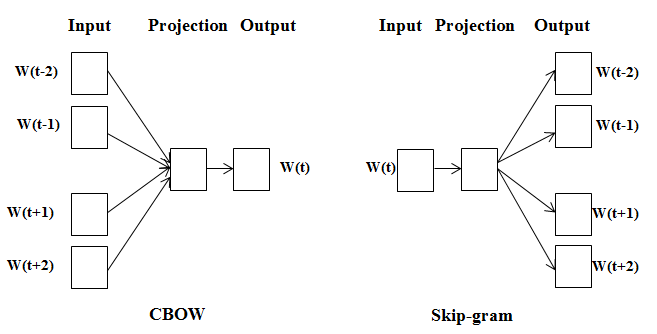
\includegraphics[width=1 \textwidth]{skipgram}
	\centering
	\caption{نمای کلی دو مدل پرش‌نگاشت و کیسه‌واژه پیوسته \citep{suleiman2017deep}}
	\label{fig.skipgram}
\end{figure}

\subsection{مبتنی ‌بر تعبیه بافت‌محور (برت)}
در بخش \ref{section.bert} با ساختار و روش آموزش مدل برت آشنا شدیم. شکل  \figurename \ref{fig.bert_embedding} 
ساختار این روش را نمایش می‌دهد.



\begin{figure}[!h]
	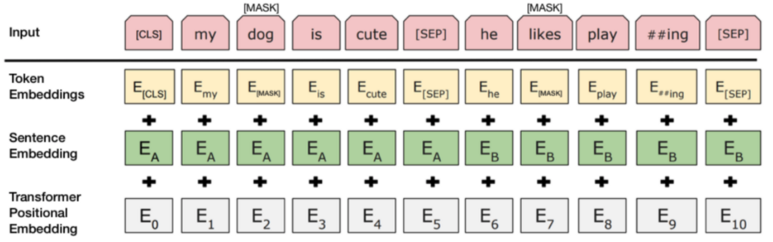
\includegraphics[width=1 \textwidth]{bert_embedding}
	\centering
	\caption{نحوه ترکیب تعبیه‌های سه‌گانه در مدل زبانی برت \citep{devlin2018bert}}
	\label{fig.bert_embedding}
\end{figure}



این مدل برای ایجاد یک بازنمایی مناسب از جملات از ترکیب سه تعبیه استفاده می‌کند که در ادامه توضیحات آنها ارائه می‌شود:
\begin{itemize}
	\item{تعبیه واژه \LTRfootnote{Token Embedding}}: منظور از تعبیه واژه تبدیل هر واژه به فضای برداری یکتا است.
	
	\item{تعبیه جمله \LTRfootnote{Sequence Embedding}}: هر داده ورودی مدل برت از دو جمله «آ» و «ب» تشکیل شده‌است که در یکی از مراحل یادگیری، این مدل برای پیش‌بینی جمله بعدی کاربرد دارد. به همین منظور، این مدل یک تعبیه برای مشخص‌کردن جمله‌ای که واژه مورد نظر در آن قرار دارد، ایجاد می‌کند.
	\item{تعبیه موقعیت انتقال‌دهنده‌ها \LTRfootnote{Transformer Positional Embedding}}: تعبیه موقعیت انتقال‌دهنده‌ها یک تعبیه از موقعیت هر واژه در جمله است که باعث می‌شود بردار حضور هر واژه در جایگاه‌های مختلف در یک جمله متفاوت باشد.
\end{itemize}

درنهایت با ترکیب این سه بخش، یک بردار ورودی برای مدل برت ساخته می‌شود که پس از مراحل یادگیری گفته‌شده در بخش قبل، برای هر جمله یک بازنمایی مناسب ارائه می‌یابد.


\subsection{بازنمایی مبتنی ‌بر موضوع (تخصیص نهان دیریکله)}
همان‌طور که در بخش \ref{section.lda_classification} بیان شد، الگوریتم تخصیص نهان دیریکله یک روش مدل‌سازی بدون‌نظارت برای تعیین موضوعات پیکره متنی است. روش عملکرد مدل‌سازی موضوع به این صورت است که پس از ورود پیکره به این الگوریتم، در نهایت ماتریس سند-موضوع و ماتریس واژه-موضوع ساخته می‌شود. به‌منظور استفاده از این روش برای یافتن یک بازنمایی مناسب برای هر سند می‌توانیم از ماتریس اول استفاده کنیم. هر سطر ماتریس سند-موضوع مرتبط با یک سند است و ستون آن احتمال هر موضوع را نشان می‌دهد. همچنین در ماتریس واژه-موضوع هر ستون یک موضوع است و هر سطر آن نیز امتیاز واژه در آن موضوع است.

%5)
\chapter{معماری مدل‌های ارائه شده}
\section{مدل‌های پایه مورد استفاده در تشخیص اخبار جعلی}
تاکنون در زبان فارسی، پژوهشگران عمدتاً از مدل‌های مرسوم یادگیری ماشین برای تشخیص اخبار جعلی استفاده کرده‌اند. یکی از اصلی‌ترین دلایل استفاده از این روش‌ها کافی نبودن داده‌های یادگیری برای آموزش مدل‌های به‌روز و پیچیده است. در این پروژه، پس از جمع‌آوری یک مجموعه داده از اخبار جعلی منتشرشده در پایگاه‌های خبری فارسی، استفاده از مدل‌های عمیق امکان‌پذیر می‌شود. به‌طورکلی پردازش داده متنی در سیستم تشخیص خبر جعلی‌ از دو بخش اصلی بازنمایی متن و دسته‌بندی متن تشکیل شده‌است که در ادامه توضیح هریک از آن‌ها ارائه می‌گردد.
\subsection{شبکه عصبی پرسپترون ساده}
شبکه عصبی شامل شبکه‌ای از عناصر پردازش ساده (نورون‌ها) است، که می‌تواند رفتار پیچیده کلی تعیین‌شده‌ای از ارتباط بین عناصر پردازش و پارامترهای عنصر را نمایش دهد. این نورون‌ها مجموعه‌ای از ویژگی‌های ورودی را گرفته و باتوجه‌ به ماتریس وزن، تمایل\LTRfootnote{Bias} و «تابع فعال‌سازی»\LTRfootnote{Activation function} خروجی را به‌دست می‌آورد. \figurename~\ref{fig.slp} نمایی از شبکه عصبی ساده را نمایش می‌دهد.

\begin{figure}[!h]
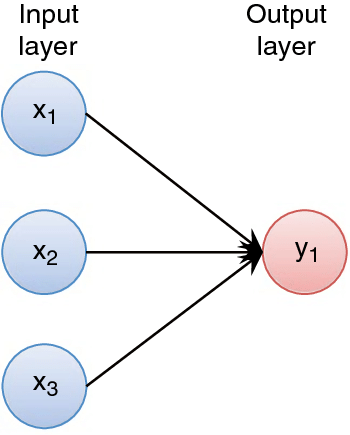
\includegraphics[width=0.25 \textwidth]{slp}
\centering
\caption{نمایی از شبکه عصبی دارای نورون‌های مدل پرسپترون ساده}
\label{fig.slp}
\end{figure}

\begin{table}[!h]
\caption{توابع فعال‌ساز پرکاربرد به‌همراه روابط و نمودار آنها}
\label{table:activationFunctions}
\begin{center}
\begin{tabular}{M{3cm}M{5cm}M{7cm}}
نام & نمودار & تعریف ریاضی \\
\hline
\hline
\lr{Binary step} &
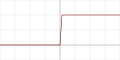
\includegraphics[scale=1]{binary_step} & 
\[f(x) =
\begin{cases}
1, & \verb|x| \geq \verb|0| \\
0, & \verb|x| < \verb|0| \\
\end{cases}
\] \\ \hline

\lr{Sigmoid} &
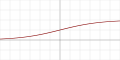
\includegraphics[scale=1]{sigmoid} & 
\[f(x) =
\frac{1}{1 +‌\exp(-x)}
\] \\ \hline

\lr{Tanh} &
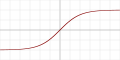
\includegraphics[scale=1]{tanh} & 
\[f(x) =
tanh(x) = \frac{\exp(x) - \exp(-x)}{\exp(x) +‌\exp(-x)}
\] \\ \hline

\lr{Relu} &
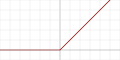
\includegraphics[scale=1]{relu} & 
\[f(x) =
\begin{cases}
x, & \verb|x| \geq \verb|0| \\
0, & \verb|x| < \verb|0| \\
\end{cases}
\] \\ \hline
\end{tabular}
\end{center}
\end{table}


توابع فعال‌ساز با استفاده از ایجاد روابط غیرخطی میان ورودی و خروجی هر نورون سعی می‌کند تا ارتباطات پیچیده‌تری را یاد بگیرد. در \tablename~\ref{table:activationFunctions} چند نمونه از این توابع فعال‌ساز با نمودار مربوط به آنها آورده شده‌است.


%==================================================================
\subsection{شبکه عصبی پیچشی}
این دسته از شبکه‌ها که در ابتدا برای حل مسائل بینایی ماشین ارائه شده بود با به‌کاربستن هسته‌هایی\LTRfootnote{Kernel} با وزن‌های مشترک روی ناحیه‌هایی از ورودی عمل پیچش را انجام می‌دهد. 

 ایده استفاده از وزن‌های‌ مشترک زمانی مطرح شد که تصاویر خاصیت ایستا دارد. این بدان معناست که آماره‌های بخش‌های مختلف یک تصویر و الگوی کلی آنچه که قرار است در تصویر تشخیص داده شود ثابت است و تغییری نمی‌کند.
 
  
 اما استفاده از شبکه‌های
 پیچشی تنها منحصر به حوزه پردازش تصویر نیست و به‌مرور وارد سایر حوزه‌ها نظیر پردازش متن نیز شده‌است.
 این نوع شبکه‌ها عمدتاً از لایه‌هایی مانند ادغام\LTRfootnote{Pool} و پیچش\LTRfootnote{Convolution} تشکیل شده‌است. لایه پیچش از فیلترهایی استفاده می‌کند که با
 انجام عملیات پیچش برروی داده ورودی، یک نگاشت ویژگی جدید تولید می‌کند. لایه ادغام نیز معمولاً پس از لایه پیچش،
 برای نمونه‌گیری از نگاشت ویژگی استفاده می‌کند. دو نوع پرکاربرد این نمونه‌گیری، «میانگین مقادیر»\LTRfootnote{Average pooling} و «بیشترین مقدار»\LTRfootnote{Max pooling} است. درنهایت پس‌از به‌دست‌آمدن نگاشت ویژگی نهایی و بردارسازی آن، از یک شبکه عصبی چند لایه استفاده می‌شود تا خروجی
 نهایی باتوجه ‌به ورودی به‌دست آید. از شبکه‌های عصبی پیچشی دو‌ بعدی، عمدتاً برای عکس و از شبکه‌های عصبی پیچشی یک‌بعدی بیشتر برای متن استفاده می‌شود. در \figurename~\ref{fig.alexnet} یک نمونه از شبکه عمیق پیچشی که برای دسته‌بندی عکس استفاده شده می‌شود نشان داده شده ‌است.

\begin{figure}[!h]
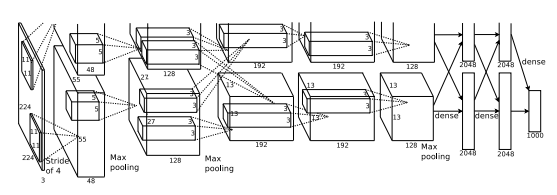
\includegraphics[width=1 \textwidth]{alexnet}
\centering
\caption{.نمای کلی مدل پیچشی الکس‌نت \citep{krizhevsky2012imagenet}}
\label{fig.alexnet}
\end{figure}

\vspace{3mm}

\begin{figure}[!h]
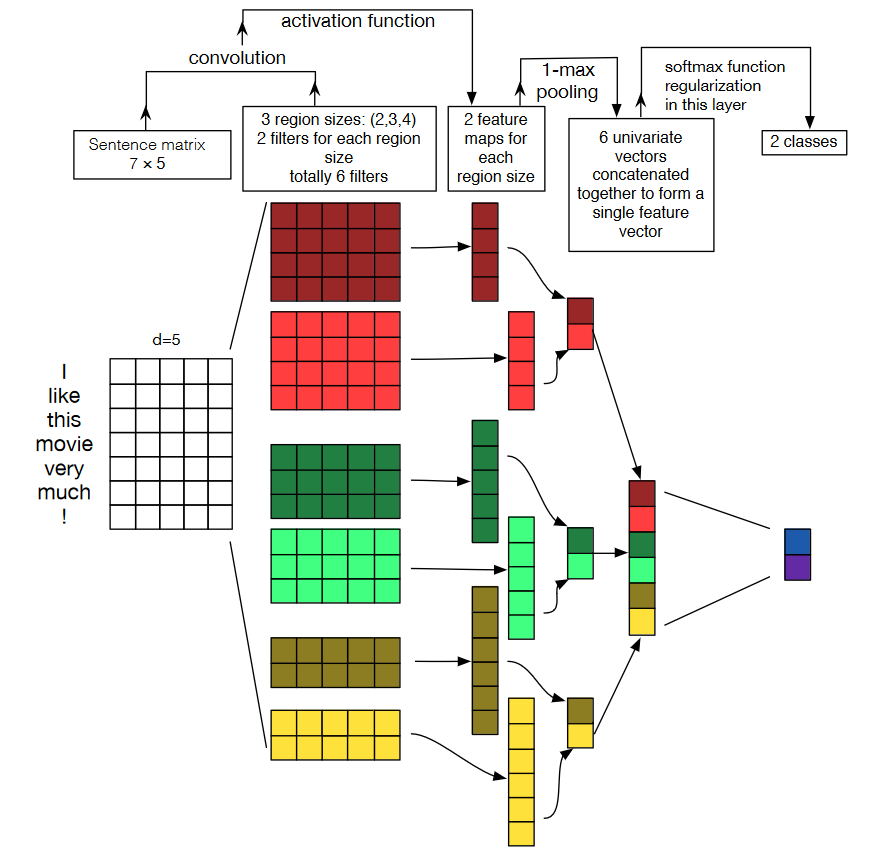
\includegraphics[width=0.85 \textwidth]{cnn}
\centering
\caption{نمای کلی یک شبکه عصبی عمیق پیچشی \citep{le2017convolutional}}
\label{fig.sentimentAnalyzing}
\end{figure}

در ادامه یک مثال کاربردی از شبکه پیچشی در زمینه پردازش متن توضیح داده می‌شود. \figurename~\ref{fig.sentimentAnalyzing} را درنظر بگیرید. یکی از مسائل  پرکاربرد در حوزه پردازش زبان طبیعی، «تحلیل احساسات»\LTRfootnote{Sentiment Analysis} است که در این مثال ما به‌طور خاص  به‌دنبال تشخیص احساس و تمایل در جمله \lr{I like this movie very much.} هستیم. در این مثال کاربردی، داده ورودی به جای یک تصویر، یک ورودی به ابعاد  $n \times d$  است که $n$ طول جمله بر حسب واژه‌ها و $d$ ابعاد تعبیه\LTRfootnote{Embedding} واژه‌ها می‌باشد. سپس در لایه پیچش، روی این ورودی هسته‌هایی با ابعاد مختلف حلقه‌ای زده می‌شود. معمولاً ابعاد این هسته‌ها برای متن ورودی یک بعدی است که این به‌معنای داشتن یک پنجره لغزان روی سطرهای ماتریس می‌باشد. به بیان دیگر، می‌توان این هسته‌ها را بازنمایی سطح بالا از چندتایی‌های واژه‌های ورودی دانست. در لایه بعد، ادغام بیشینه روی خروجی مرحله قبل  انجام شده و خروجی آن‌ها نیز برای دسته‌بندی به لایه تماماً متصل داده می‌شود. در مسئله تحلیل احساس می‌توان فرض کرد که عبارت \lr{like this movie} (که مهم‌ترین عامل نشان‌دهنده احساس است)  در هر جای متن  به‌عنوان احساس مثبت درنظر گرفته‌شده و مکان این عبارت برای تصمیم‌گیری درمورد دسته‌بندی آن اهمیتی ندارد. بنابراین، با حرکت آن پنجره لغزان می‌توان عبارات مثبت را شناخت؛ و درنهایت می‌توان با استفاده از این اطلاعات، مثبت یا منفی بودن احساس کل عبارت را مشخص نمود.

%==================================================================

\section{مدل‌های بازنمائی متن مبتنی بر بافت}
\label{section.pretrained_models}
اولین قدم برای پردازش متن، ایجاد بازنمایی مناسب برای متن ورودی است. در این بخش به بررسی مدل‌های زبانی برت \citep{devlin2018bert} و مدل‌های مبتنی بر معماری آن مانند برت چند زبانه \LTRfootnote{Multilingual BERT}، پارس‌برت \LTRfootnote{ParsBERT} \citep{ParsBERT}، آلبرت‌-فارسی \LTRfootnote{ALBERT-Persian} \citep{ALBERTPersian}، ایکس.ال.ام-روبرتا \LTRfootnote{XLM-RoBERTa} \citep{conneau2019unsupervised} می‌پردازیم.

\subsection{برت}
\label{section.bert}
\citet{devlin2018bert} 
یک مدل زبانی جدید با نام برت را معرفی کردند. ایده اصلی این مدل استفاده از انتقال‌دهنده‌های‌\LTRfootnote{Transformer} دوطرفه برای یادگیری معنا و ساختار واژه‌های موجود در متن است. مدل برت به‌صورت دو نسخه «برت پایه»\LTRfootnote{BERT-Base} و «برت بزرگ»\LTRfootnote{BERT-Large} معرفی شده‌است. برت پایه دارای 12 لایه انتقال‌دهنده و  110 میلیون پارامتر و برت بزرگ دارای  24 لایه و 340 میلیون پارامتر است. انتقال‌دهنده‌ها از «مکانیزم توجه»\LTRfootnote{Attention mechanism} در فرایند یادگیری استفاده می‌کند و سعی می‌کند تا ارتباط مفهومی میان واژه‌های موجود در یک جمله را به‌درستی یاد بگیرد. فرایند یادگیری مدل‌های زبانی عموماً به این صورت است که تلاش می‌کند تا واژه بعدی یک دنباله را حدس بزند و بر این اساس، ارتباط میان واژه‌ها را تشخیص دهند. اما در مدل زبانی برت که به‌صورت دوطرفه (چپ‌به‌راست و راست‌به‌چپ) متن را بررسی می‌کند نمی‌توان فقط از این روش استفاده کرد. برای آموزش مدل برت دو مرحله زیر برروی پیکره‌های متنی ویکی‌پدیا و کتاب‌ها اعمال شده‌است. 
 در \figurename~\ref{fig.BERT} نحوه آموزش در مدل برت نمایش داده شده‌است.

\begin{figure}[!h]
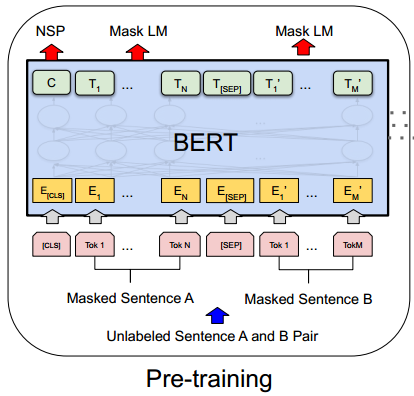
\includegraphics[width=0.6 \textwidth]{bert}
\centering
\caption{ نحوه عملکرد یادگیری مدل برت \citep{devlin2018bert}}
\label{fig.BERT}
\end{figure}

\begin{itemize}
\item \textbf{پوشش واژه‌ها} \\
قبل از استفاده از داده‌ها در شروع فرایند یادگیری، 15 درصد از واژه‌های داخل متن به‌صورت تصادفی انتخاب می‌شود. 
 از این حجم واژه‌ها 80‌ درصد واژه‌ها با عبارت \verb|[MASK]| جایگزین شده و 10 درصد با یک واژه تصادفی جایگزین می‌شود و 10
 درصد دیگر بدون تغییر باقی می‌ماند. در ادامه، مدل سعی می‌کند تا با استفاده از اطلاعات زمینه‌ای، این واژه‌ها را حدس بزند.
 این کار با اضافه‌کردن یک لایه پس از لایه کدگذار مدل برت انجام می‌شود تا با استفاده از آن، احتمال وجود هریک از واژه‌ها
 مشخص شود و با داشتن واژه اصلی، خطای مدل حساب شده و تمامی وزن‌ها به‌روزرسانی می‌شود.

\item \textbf{پیش‌بینی جمله بعدی} \\
در این حالت، مدل برت یک جفت دنباله مانند آ و ب را دریافت می‌کند. در ابتدا و انتها جملات عبارات \verb|[CLS]| و \verb|[SEP]| قرار
 می‌گیرد. پس از اضافه‌کردن نوع جمله ($آ$ یا $ب$) به ویژگی‌های نهفته هر جمله، تمامی ورودی‌ها وارد انتقال‌دهنده‌ها شده و
 درنهایت با استفاده از یک لایه، مقدار احتمال ظهور دنباله $ب$ به‌عنوان جمله بعدی دنباله $آ$ مشخص می‌شود. با این روش مدل برت
 تلاش می‌کند تا مفاهیم زمینه‌ای را به‌طور کامل میان واژه‌ها و عبارات یاد بگیرد.
\end{itemize}

درنهایت پس از آماده‌شدن مدل زبانی، می‌توانیم از آن در مسائل مختلف مانند دسته‌بندی متن، پرسش و پاسخ\LTRfootnote{Question Answering (QA)} و تشخیص
 موجودیت‌های نامدار\LTRfootnote{Name Entity Recognition (NER)} استفاده کنیم.


\subsection{برت چند زبانه}
	مدل زبانی برت چند زبانه \citep{devlin2018bert} با استفاده از داده‌هایی از ۱۰۴ زبان مختلف شامل زبان فارسی آموزش داده شده‌است. مدل زبانی برت دارای دو نوع پایه و بزرگ است که ما در این پروژه از مدل برت پایه، شامل ۱۲ لایه انتقال‌دهنده و ۱۱۰ میلیون پارامتر استفاده کرده‌ایم. این مدل با استفاده از پیکره متنی ویکی‌پدیا\LTRfootnote{Wikipedia} که به زبان‌های مختلف موجود است، آموزش داده شده‌است. 
	
\subsection{پارس‌برت}
	\cite{ParsBERT}
	مدل زبانی پارس‌برت که مبتنی بر معماری مدل برت است،انحصاراً برای زبان فارسی آموزش داده شده‌است. این مدل عملکرد بهتری نسبت‌به مدل‌های چند زبانی مانند برت داشته‌است. همچنین به‌دلیل آنکه این مدل تنها برای زبان فارسی ارائه شده‌است، سبک‌تر از مدل زبانی برت چندزبانه است. به‌منظور آموزش مدل‌زبانی پارس‌برت از منابع متنی موجود در وب‌سایت‌های ویکی‌پدیا، بیگ‌بنگ، چطور، الی‌گشت، دیجی‌کالا، تد‌تاک، کتاب‌ها و پیکره میراث استفاده شده‌است. همچنین برای ارزیابی مدل‌ ارائه‌شده در پارس‌برت از تحلیل احساسات، تشخیص موجودیت‌های نامدار و دسته‌بندی متن استفاده شده‌است.
	
\subsection{آلبرت-فارسی}
	مدل‌زبانی آلبرت یک نسخه سبک‌تر از برت است که معماری کاملاً مشابه‌ای با آن دارد که در پیاده‌سازی آن تغییر اندکی نسبت ‌به مدل برت وجود دارد \citep{ALBERTPersian}. آلبرت-فارسی، مانند مدل‌زبانی پارس‌برت بر روی  پیکره‌های متنی فارسی آموزش داده شده‌است. علیرغم اینکه منابع این پیکره‌های فارسی مشابه مدل‌زبانی پارس‌برت است، به ‌مراتب حجم  کمتری نسبت ‌به پارس‌برت دارد.
	
\subsection{ایکس.ال.ام-روبرتا}
	با توجه به موفقیت‌های چشمگیر مدل‌های ازپیش آموزش‌دیده، \cite{conneau2019unsupervised} یک مدل‌ بین‌زبانی ارائه کردند که توانست دقت بهتری را در مقایسه با مدل‌های زبانی رایج مانند برت ثبت کند. این مدل که بر روی دادگان ۱۰۰ زبان مختلف ازجمله فارسی آموزش داده شده‌است  با استفاده از ۳ روش آموزش داده می‌شود: (۱) پیش‌بینی کلمه بعدی، (۲) پیش‌بینی کلمه پوشیده شده و (۳) مدل زبانی مبتنی بر ترجمه.
%==================================================================

\section{معماری‌های پیشنهادی برای تشخیص اخبار جعلی}
به طور کلی، مدل‌های بازنمائی متن مبتنی بر بافت خروجی‌های متفاوتی را می‌توانند ایجاد کنند. مدل‌هایی با ساختار مشابه برت مانند پارس‌برت، آلبرت-فارسی و برت چند زبانه ۲ نوع بازنمائی برای متن ورودی ایجاد می‌کنند:
\begin{itemize}
\item بازنمایی تجمعی\LTRfootnote{Pooled} به ازای هر دنباله از واژه‌های ورودی، یک بازنمایی کلی برای کل دنباله ارائه می‌کند.
این بازنمائی تنها توسط مدل‌های مبتنی بر ساختار برت ایجاد می‌شود.
\item بازنمایی دنباله‌ای\LTRfootnote{Sequence} که در آن برای هر واژه یک بردار بازنمایی مبتنی‌بر بافت ارائه
 می‌گردد. برخلاف بازنمائی تجمعی، بازنمائی دنباله‌ای را تمامی مدل‌های بازنمائی متن مبتنی بر بافت تولید می‌کنند.
\end{itemize}

در این پروژه، رویکرد پیشنهادی دو معماری مختلف مورد استفاده قرار گرفته‌است که در هر یک از این معماری‌ها، یکی از دو حالت فوق به‌کار رفته‌است. در روش اول با استفاده از یک مدل پرسپترون ساده به دسته‌بندی اخبار بازنمائی شده توسط بردار‌های تجمعی می‌پردازیم و در روش دوم با استفاده از یک شبکه‌‌عصبی پیچشی به استخراج ویژگی‌های سطح بالاتر از هم‌نشینی واژگان یک خبر می‌پردازیم و درنهایت با استفاده از یک لایه چگال، اخبار دسته‌بندی می‌شوند.


%==================================================================

\subsection{مدل زبانی مبتنی بر بافت + پرسپترون ساده}
برای استفاده از مدل‌‌های مبتنی بر بافت در مسئله دسته‌بندی کافی است تا از بردار خروجی متناظر با توکن \verb|[CLS]| به‌عنوان بردار نماینده آن دنباله استفاده کنیم. دلیل استفاده از این بردار این است که شامل تمامی بردارهای توکن‌های موجود در متن است، درحالی‌که بردارهای متناظر با توکن‌های دیگر تنها نماینده آن توکن در عبارت ورودی است. بنابراین کافی است تا بردار نماینده دنباله متنی ورودی را وارد یک لایه تکی پرسپترون کنیم که می‌تواند عمل تشخیص برچسب دنباله ورودی را برای ما انجام دهد. این ساختار با استفاده از مدل زبانی برت در \figurename~\ref{fig.bertSLP} ترسیم شده‌است.

به عبارت دیگر، با استفاده از بازنمایی به‌دست‌آمده از مدل برت برای یک جمله و داشتن برچسب آن سعی می‌کنیم تا با استفاده از  دادگان موجود، یک مدل کامل برای تشخیص اخبار جعلی بسازیم. برای این هدف کافی است تا وزن‌های ورودی به لایه پرسپترون  ساده آموزش داده شود به صورتی که بتواند اخبار را به درستی دسته‌بندی کند. 

\begin{figure}[!h]
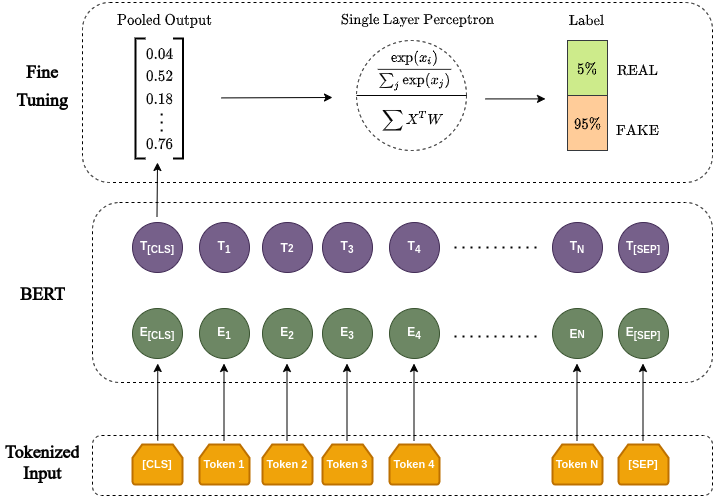
\includegraphics[width=0.75 \textwidth]{bert_slp}
\centering
\caption{نحوه استفاده از یک لایه پرسپترون ساده درکنار مدل برت}
\label{fig.bertSLP}
\end{figure}
\noindent

به‌منظور جلوگیری از بیش‌برازش\LTRfootnote{Overfitting} شدن مدل، از روش «حذف تصادفی نورون‌ها»\LTRfootnote{Dropout} استفاده می‌کنیم تا مدل نهایی تا حد ممکن ساده باشد و به‌درستی ویژگی‌های مهم را یاد بگیرد. در انتهایی‌ترین بخش مدل هم یک لایه نورون به تعداد دسته‌های دادگان ورودی وجود دارد که تابع فعال‌ساز آنها بیشینه هموار است چراکه نیاز داریم تا احتمال تعلق‌داشتن خبر به هر دسته را بدانیم و بیشترین آن را به‌عنوان برچسب پیشبینی‌شده اعلام نماییم.

تابع «خطا آنتروپی متقاطع طبقه‌ای»\LTRfootnote{ Categorical Cross-entropy} نیز برای محاسبه میزان خطای پیش‌بینی مدل دسته‌بند خبر جعلی استفاده شده‌است که رابطه ریاضی آن در زیر آمده‌است.

\begin{equation}
Loss = - \sum_{c=1}^{M}y_{o,c} . log(p_{o,c})
\end{equation}
در این رابطه، $M$ تعداد دسته‌ها و $y_o$ بردار تک‌روشن از برچسب خبر $o$ است و $p_o$ نیز بردار احتمال پیش‌بینی‌شده توسط مدل است که نشان‌دهنده احتمال تعلق به هر دسته است.

%==================================================================

\subsection{مدل زبانی مبتنی بر بافت + پیچشی}
با استفاده از خروجی دنباله‌ای یک مدل‌ بازنمائی مبتنی بر بافت و اتصال آن به یک شبکه عصبی پیچشی، عملیات نگاشت ویژگی انجام داده می‌شود. پس‌از عملیات یادگیری، این مدل سعی می‌کند تا با تبدیل بازنمایی تولیدشده به یک بازنمایی دیگر، عملیات پیش‌بینی کذب‌بودن یا اصیل‌بودن یک خبر را انجام دهد. در این مدل، به‌جای بردار خروجی تجمعی، از بردار خروجی دنباله‌ای که شامل دنباله‌ای از بردارهای تک‌تک واژه‌های داخل خبر است استفاده می‌گردد؛ چراکه با استفاده از لایه‌های پیچشیِ پس‌از آن می‌توان همنشینی‌هایی از واژه‌ها که نشان‌دهنده اخبار جعلی است را شناسایی کرد. برای این منظور، از سه لایه پیچشی موازی شامل ۳۰ فیلتر با اندازه‌های ۳، ۴ و ۵ استفاده می‌کنیم. همچنین تابع فعال‌ساز این لایه، تابع «یک‌سوساز خطی»\LTRfootnote{ReLU} است. پس از این لایه، یک لایه ادغامِ بیشترین مقدار قرار دارد تا با استفاده از عملیات «نمونه‌کاهی»\LTRfootnote{Downsampling}، ویژگی‌های مناسب را استخراج کند. درنهایت، با استفاده از یک «لایه تخت‌شونده»\LTRfootnote{Flatten layer}، ماتریس مرحله قبل به یک بردار یک بعدی تبدیل می‌شود تا با استفاده از یک لایه چگال\LTRfootnote{Dense} با استفاده از تابع فعال‌ساز «بیشینه هموار»\LTRfootnote{Softmax}، احتمال هر دسته مشخص شود. \figurename~\ref{fig.bertCNN} نحوه اتصالات و به‌دست‌آوردن ویژگی‌های سطح بالاتر با استفاده از مدل زبانی برت را نشان می‌دهد.

\begin{figure}[!h]
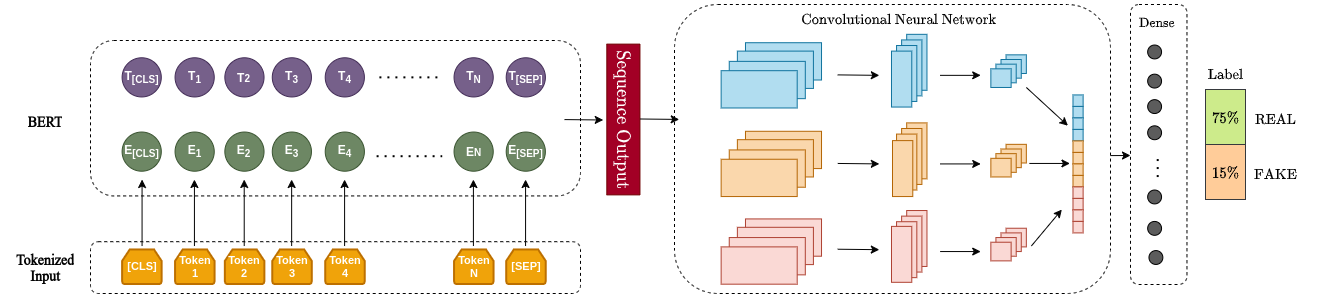
\includegraphics[width=1 \textwidth]{bert_cnn}
\centering
\caption{نحوه ارتباط لایه پیچشی با بردارهای خروجی مدل برت}
\label{fig.bertCNN}
\end{figure}

%6)
\chapter{بررسی نتایج و ارزیابی مدل‌های ارائه شده}


\section{آزمایش‌های انجام‌شده بر روی پیکره «تاج»}
پس از استخراج یک مجموعه داده در حوزه اخبار جعلی، به ارزیابی مدل‌های ارائه شده می‌پردازیم. همانطور که در بخش \ref{section.pretrained_models} عنوان شد، چندین مدل از پیش آموزش‌ دیده برای زبان‌ فارسی موجود است. در این بخش ما با استفاده از دسته‌بند‌های ذکرشده، پیچشی و پرسپترون، یک مقایسه میان این مدل‌ها انجام می‌دهیم تا بهترین مدل‌ را برای تشخیص اخبار جعلی فارسی انتخاب کنیم. به منظور اثبات کارایی مدل‌های ارائه‌شده، ما از دادگان دیگر فارسی و انگلیسی نیز برای ارزیابی استفاده می‌کنیم.

\subsection{تنظیمات آزمایش‌ها}
مدل‌های برت چندزبانه و ایکس.ال.ام-روبرتا دارای نسخه‌های متفاوتی است. در این پژوهش، ما از نسخه‌ پایه هر دو مدل استفاده کردیم. مدل برت چند‌زبانه پایه دارای ۱۷۹ میلیون پارامتر قابل آموزش، ۱۲ لایه انتقال‌دهنده و لایه میانی با اندازه ۷۶۸ است. مدل ایکس.ال.ام-روبرتا پایه نیز دارای ۲۷۰ میلیون پارامتر، ۱۲ لایه انتقال‌دهنده و لایه‌میانی با اندازه ۷۶۸ است. مدل‌های دیگر مانند پارس‌برت و آلبرتا-فارسی همگی بر پایه مدل برت است.

معماری دسته‌بند پیچشی شامل ۳ لایه پیچشی موازی شامل ۳۰ فیلتر‌ با ابعاد متفاوت ۳ و ۴ و ۵ است که ویژگی‌های سطح بالاتر را از ماتریس خروجی مدل ازپیش‌ آموزش‌دیده که شامل یک بردار مجزا برای هر کلمه ورودی است، استخراج می‌کند. لایه آخر این دسته‌بند نیز یک پرسپترون ساده است که با استفاده از تابع بیشینه‌هموار\LTRfootnote{Softmax}، برچسب هر خبر را مشخص می‌کند. به‌منظور جلوگیری از مشکل بیش‌برازش\LTRfootnote{Overfit} در مدل نیز از پارامتر‌های تنظیم‌کننده در فیلتر‌ها استفاده شده ‌است.

شبکه عصبی پیشرو پرسپترون نیز شامل یک لایه پرسپترون با تابع فعال‌ساز بیشینه‌هموار است که با استفاده از بردار خروجی مدل از پیش آموزش‌ دیده به محاسبه احتمال تعلق یک خبر به هر کدام از دسته‌ها می‌پردازد.

در تمامی مدل‌ها نیز یک لایه بیرون‌انداز\LTRfootnote{Dropout Layer} قبل از لایه‌ نهایی قرار گرفته‌ است. همچنین در آموزش مدل‌ها نرخ یادگیری\LTRfootnote{Learning Rate} در آموزش برابر با $5e-5$، تعداد دوره‌‌ها\LTRfootnote{Epoch} برابر با ۴ و مقدار اندازه دسته\LTRfootnote{Batch Size} ۶۴  است.

\subsection{نتایج}
جدول \ref{table.text_result_cnn} نتایج ارزیابی مدل‌های ارائه‌شده با استفاده از مدل‌های از پیش آموزش‌ دیده متفاوت و با استفاده از شبکه عصبی پیچشی را نمایش می‌دهد. طبق نتایج به‌دست‌آمده می‌توان نتیجه گرفت که مدل پارس‌برت نسبت‌ به بقیه‌ مدل‌ها توانسته‌ است متن‌های ورودی را دقیق‌تر بازنمایی کند و ما با استفاده از این مدل می‌توانیم اخبار جعلی را با دقت بالاتری نسبت‌به سایر مدل‌ها تشخیص دهیم.

\begin{table}
	\caption{نتایج تشخیص اخبار جعلی فارسی با استفاده از بازنمایی‌های مختلف و دسته‌بندی با شبکه عصبی پیچشی}
	\label{table.text_result_cnn}
	\begin{center}
		\begin{tabular}{|c|c|c|c|c|}
			\hline
مدل & فراخوانی & صحت & معیار اف & دقت \\
			\hline
			\hline
برت چندزبانه & $88.55$ & $84$ & $86.21$ & $87.33$\\
			\hline
آلبرت-فارسی & $87.02$ & $92$ & $89.44$ & $89.75$ \\
			\hline
پارس برت & $89.13$ & $93.71$ & $91.36$ & $91,64$ \\
			\hline
ایکس.ال.ام-روبرتا & $87.84$ & $90.85$ & $89.32$ & $89.75$ \\
			\hline
		\end{tabular}
	\end{center}
\end{table}

در گام بعدی، در مدل پارس برت علاوه‌بر دسته‌بندی با شبکه پیچشی، دسته‌بندی با شبکه پیشرو پرسپترون تک‌لایه نیز مورد بررسی قرار گرفت که نتایج آن در جدول \ref{table.text_result_slp} گزارش شده‌ است. همان‌طور که نتایج این جدول نشان می‌دهد شبکه پرسپترون تک‌لایه به نتایج نزدیکی در مقایسه با شبکه پیچشی رسیده‌ است و با تفاوت اندک به دقت و معیار اف بالاتری دست یافته ‌است. بر اساس این نتایج، بازنمایی پارس‌برت در سطح واژه به‌ همراه شبکه پیچشی و بازنمایی پارس‌برت در سطح متن به همراه شبکه پیشرو پرسپترون در گام‌های بعدی این پروژه مورد استفاده قرار خواهد گرفت.

\begin{table}
	\caption{نتایج تشخیص اخبار جعلی فارسی با استفاده از بازنمایی پارس‌برت و مقایسه دسته‌بندها}
	\label{table.text_result_slp}
	\begin{center}
		\begin{tabular}{|c|c|c|c|c|c|}
			\hline
مدل & دسته‌بند & فراخوانی & صحت & معیار اف & دقت \\
			\hline
			\hline
پارس برت & شبکه عصبی پیچشی  & $89.13$ & $93.71$ & $91.36$ & $91.64$ \\
			\hline
پارس برت & شبکه پیشرو پرسپترون تک‌لایه & $92.44$ & $90.85$ & $91.64$ & $92.18$ \\
			\hline
		\end{tabular}
	\end{center}
\end{table}

\section{آزمایش‌های انجام‌شده بر روی سایر پیکره‌های فارسی}
همانطور که ذکر شد، از آنجا که دادگان تهیه‌شده در این پروژه برای اولین بار در زمینه تشخیص خبر جعلی مورد استفاده قرار می‌گیرد، نتایج پایه دیگری بر روی این دادگان به‌منظور مقایسه وجود ندارد. بر همین اساس، به‌‌منظور ارزیابی مدل‌های ارائه‌شده برای زبان فارسی و مقایسه نتایج این پروژه با کارهای قبلی انجام‌شده در زبان فارسی، ما از دو مجموعه داده موجود برای تشخیص شایعات در شبکه‌های اجتماعی توییتر و تلگرام استفاده کردیم. مدل‌های پایه‌ای که برای مقایسه استفاده شده ‌است در ادامه مرور می‌شوند:
\begin{itemize}
\item
\cite{zamani2017rumor}
یک روش مبتنی‌ بر مدل «بهینه‌سازی کمینه متوالی»\LTRfootnote{Sequetional Minimal Optimization (SMO)} که یک روش آموزش ماشین بردار پشتیبان است برای تشخیص شایعات فارسی در شبکه اجتماعی تلگرام ارائه داده‌اند. ما در این بخش از آزمایش‌ها مدل ارائه‌شده در این پروژه را با مدل ارائه‌شده توسط \cite{zamani2017rumor} مقایسه نموده‌ایم. در این مقایسه از دادگانی که توسط \cite{zamani2017rumor} ارائه گردیده است استفاده کرده‌ایم. شایان ذکر است در مقاله ارائه‌شده توسط ایشان، علاوه بر اطلاعات متنی، از ویژگی‌های مرتبط با گراف کاربران توییتر نیز استفاده کرده‌اند، اما به‌دلیل عدم دسترسی به این اطلاعات، مقایسه ما تنها با بخشی از مدل‌های ارائه‌شده توسط \cite{zamani2017rumor}  که برروی دادگان متنی پیاده شده است  انجام پذیرفته ‌است.

\item
\citet{jahanbakhsh2020model}
با ارائه مدل مبتنی‌ بر ماشین بردار پشتیبان به دسته‌بندی شایعات در شبکه اجتماعی توییتر پرداختند. ما در بخش دیگری از آزمایش‌ها از دادگان توییتر ارائه‌شده توسط \citet{jahanbakhsh2020model} استفاده کردیم و مدل خود را با نتایج آن‌ها مقایسه نمودیم.

جدول \ref{table.comparison} نتایج حاصل از مدل‌های پیاده‌شده در این پژوهش را بر روی دو مجموعه داده حاصل از تلگرام و توییتر نشان می‌دهد. در این آزمایش‌ها از مدل زبانی پارس‌برت استفاده شده‌است.


\begin{table}
	\caption{ارزیابی و مقایسه مدل‌های ارائه‌شده با مدل‌های پیشین برروی دادگان فارسی شبکه‌های اجتماعی}
	\label{table.comparison}
	\begin{center}
		\begin{tabular}{|c|c|c|c|c|c|}
			\hline
			مدل & دادگان & فراخوانی & صحت & معیار اف & دقت \\
			\hline
			\hline
			\citep{zamani2017rumor} & 
			\multirow{4}{*}{توییتر} &$71.44$&$81.24$& $76.02$ & $74.26$ \\
			
			\cline{1-1}
			\cline{3-6}
			\citep{jahanbakhsh2020model} &
			 & $76.3$ & $76.3$ & $76.3$ & - \\
			\cline{1-1}
			\cline{3-6}
			پارس‌برت - پیچشی & & $95.71$ & $97.10$ & $96.40$ & $96.12$ \\
			\cline{1-1}
			\cline{3-6}
			پارس‌برت - پرسپترون & & $94.20$ & $94.20$ & $94.20$ & $93.79$ \\
			\hline
			\citep{jahanbakhsh2020model} &
			\multirow{3}{*}{تلگرام}& $82.8$ & $82.9$ & $82.8$ & - \\
			\cline{1-1}
			\cline{3-6}
			پارس‌برت - پیچشی & & $93.49$ & $95.04$ & $94.26$ & $92.51$ \\
			\cline{1-1}
			\cline{3-6}
			پارس‌برت - پرسپترون & & $92.06$ & $95.86$ & $93.92$ & $91.97$ \\
			\hline
		\end{tabular}
	\end{center}
\end{table}
\end{itemize}
	
	همانطور که از نتایج مشخص است، مدل‌های ارائه شده با استفاده از بازنمائی‌ مبتنی بر مفهوم به صورت چشمگیری معیار‌های ارزیابی را بهبود دادند. همچنین، دسته‌بند پیچشی درمقایسه با مدل شبکه پرسپترون پیشرو عملکرد بهتری داشته است چراکه در این حالت مدل پیچشی ویژگی‌های سطح بالاتری را براساس هم‌نشینی واژگان ایجاد می‌کند. با توجه به آزمایش‌های انجام شده برروی دادگان توییتر، مدل پارس‌برت-پیچشی ۲۰ درصد معیار اف را در مقایسه با مدل‌های ارائه شده توسط \cite{zamani2017rumor} و \cite{jahanbakhsh2020model} بهبود‌ داده‌است. علاوه بر این، این مدل توانست برروی دادگان تلگرام نیز معیار اف را در مقایسه با نتایج بدست‌آمده توسط \cite{jahanbakhsh2020model} 
	۱۱ درصد ارتقا دهد.
	
\section{آزمایش‌های انجام‌شده برروی پیکره‌های زبان انگلیسی}
همان‌طورکه پیش‌تر مطرح شد، برای تشخیص خبر جعلی فارسی ابتدا شاکله‌ی یک مدل را براساس داده انگلیسی می‌سازیم و سپس با تغییر داده به فارسی، مدل را با داده فارسی آموزش داده و آن را بهینه می‌کنیم. ازاین‌رو، در ادامه، مدل آموزش‌ داده‌ شده با داده انگلیسی توضیح داده می‌شود. برای استفاده از دادگان لیار از ویژگی متن خبر و ۵ ویژگی مرتبط با تاریخچه اعتبار هر عنوان خبر استفاده می‌گردد. 
تاریخچه اعتبار هر گوینده شامل تعداد اخبار «به‌سختی درست»، «جعلی»، «نیمه درست»، «عمدتاً درست» و «دروغ» که از این گوینده تا کنون منتشر شده‌است می‌باشد.
علاوه بر آنها، تمامی ۶ برچسب که پیش‌تر معرفی شده بود به ۲ دسته «جعلی» و «اصیل» نگاشت می‌شود و برچسب زده می‌شوند؛
به این صورت که برچسب‌های «درست»، «نیمه درست» و «عمدتاً درست» به دسته اصیل و برچسب‌های «جعلی»،  «دروغ» و «به‌سختی درست» به دسته جعلی نگاشت می‌شوند.  در \tablename~\ref{table.LiarResults2} نتایج حاصل از ارزیابی این دادگان در حالت ۲ برچسب «جعلی» و «اصیل» با استفاده از دو مدل برت و شبکه عصبی پیچشی نمایش داده شده‌است. در این جدول، مدل حاصل از شبکه پیچشی که از ورد۲وک\LTRfootnote{Word2vec}\citep{mikolov2013distributed} برای تعبیه‌ واژه‌ها استفاده شده‌است به‌عنوان مدل پایه مورد استفاده و مقایسه قرار گرفته‌است.  همچنین در \figurename~\ref{LIAR-CM} ماتریس درهم‌ریختگی دو مدل «برت + پرسپترون ساده» و «برت +‌ پیچشی» و مدل پایه نمایش داده شده‌است.

\begin{table}[!h]
	\caption{نتایج آزمایش مدل‌های ارائه‌شده بر روی دادگان لیار (۲ برچسب)}
	\label{table.LiarResults2}
	\begin{center}
		\begin{tabular}{|M{4cm}|c|c|c|c|c|}
			\hline
			مدل & بازنمایی & فراخوانی & صحت & دقت & معیار اف \\
			\hline
			\hline
			شبکه عصبی پیچشی‌ & 
			ورد۲وک & 
			$58.58$ &
			$48.14$ & 
			$54.34$ & 
			$52.84$ \\
			\hline
			شبکه عصبی پیچشی‌ & 
			برت & 
			$62.92$ &
			$67.05$ & 
			$70.30$ & 
			$64.91$ \\
			\hline
			پرسپترون ساده & 
			برت & 
			$64.37$ &
			$66.04$ & 
			$69.98$ & 
			$65.19$ \\
			\hline
		\end{tabular}
	\end{center}
\end{table}

\begin{table}[!h]
	\caption{ مقایسه مدل‌های ارائه شده با مدل‌های پایه براساس دادگان لیار (۶ برچسب)}
	\label{table.LiarResults6}
	\begin{center}
		\begin{tabular}{|M{6cm}|c|c|c|}
			\hline
			مدل & بازنمایی & دقت تست & دقت اعتبارسنجی \\
			\hline
			\hline
			ال.اس.تی.ام مکانیزم توجه  &
			\multirow{2}{*}{ورد۲وک} &
			\multirow{2}{*}{$38.5$} &
			\multirow{2}{*}{$37.8$} \\
			\citep{long2017fake} &  &  &  \\
			\hline
			
			شبکه کپسولی &
			\multirow{2}{*}{ورد۲وک}&
			\multirow{2}{*}{$39.5$} &
			\multirow{2}{*}{$40.9$}\\
			\citep{goldani2020detecting} & &  & \\
			\hline\hline
			
			\multirow{2}{*}{شبکه عصبی پیچشی}& 
			ورد۲وک & 
			$39.3$ &
			$39.8$ \\
			\cline{2-4}
			& 
			برت & 
			$44.1$ &
			$45.5$ \\
			\hline
			پرسپترون ساده & 
			برت & 
			\textbf{$45.1$} &
			\textbf{$48.4$} \\
			\hline
		\end{tabular}
	\end{center}
\end{table}

\begin{figure}[!h]
	\centering
	\begin{tabular}{ccc}
		\begin{subfigure}{0.33\textwidth}
			\centering
			\caption{ورد۲وک + پیچشی}
			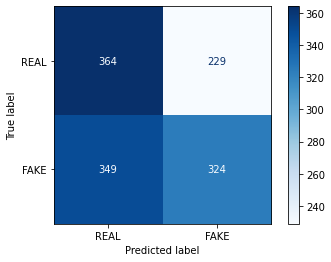
\includegraphics[width=1 \textwidth]{cnn-liar2-cm}
		\end{subfigure}
		& 
		\begin{subfigure}{0.33\textwidth}
			\centering
			\caption{برت + پیچشی}
			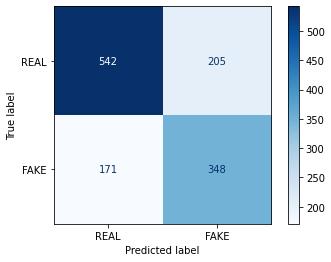
\includegraphics[width=1 \textwidth]{bert-cnn-liar2-cm}
		\end{subfigure}
		&
		\begin{subfigure}{0.33\textwidth}
			\centering
			\caption{برت + پرسپترون ساده}
			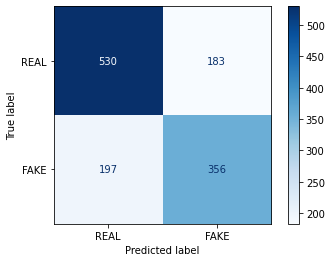
\includegraphics[width=1 \textwidth]{bert-slp-liar2-cm}
		\end{subfigure}
	\end{tabular}
	\caption{ ماتریس درهم‌ریختگی نتایج آزمایش‌های دادگان لیار}
	\label{LIAR-CM}
\end{figure}

همان‌طورکه در \tablename~\ref{table.LiarResults2}  مشاهده می‌شود، مدل پرسپترون ساده با استفاده از بازنمایی تولیدشده توسط مدل برت نتیجه بهتری را برای این مجموعه دادگان داشته‌ و با دقت بالاتری اخبار جعلی را تشخیص داده‌است.  در این مدل، میزان خطای مثبت کاذب که نشانگر تعداد اخبار جعلی است که توسط سیستم به خطا اصیل تشخیص داده شده‌است کمتر از سایر مدل پیشنهادی ما می‌باشد.

برای مقایسه مدل پیشنهادی با سایر مدل‌های مطرح و به‌ روز، نتایج آزمایش مدل‌های این طرح با مدل‌هایی که پیش‌تر برای دسته‌بندی اخبار دادگان لیار با ۶ برچسب ارائه شده‌ است در\tablename~ \ref{table.error_liar_fn} نمایش داده شده‌ است.  باتوجه‌به نتایج، مدل پرسپترون ساده با استفاده از بازنمایی برت نسبت‌به دیگر مدل‌ها با دقت بالاتری اخبار لیار را دسته‌بندی کرده ‌است.

برای بررسی خطا در مدل‌های ارائه شده، در ادامه دو نمونه از اخباری که به اشتباه در آزمایش مدل «برت + پرسپترون» دسته‌بندی شده‌است، مورد بررسی قرار می‌گیرد. ابتدا سابقه گوینده‌ی هر دو خبر در  \tablename~\ref{table.error_history_liar_fn}  نمایش داده شده‌ است.  در ادامه  \tablename~\ref{table.error_liar_fn}   آمار واژگان نمونه  (۱)   را نمایش می‌دهد که یک خبر جعلی است و به اشتباه در دسته اخبار اصیل قرار گرفته‌است. همچنین  \tablename~\ref{table.error_liar_fp}   آمار واژگان نمونه  (۲)   را نشان می‌دهد که یک خبر اصیل است و به اشتباه در دسته جعلی قرار گرفته‌است. 



(۱)\\
\begin{flushleft}\lr{Citizens Property Insurance has over \$500 billion worth of risk, with less than \$10 billion worth of surplus.}\end{flushleft}

(۲)\\
\begin{flushleft}\lr{Says the unemployment rate for college graduates is 4.4 percent and over 10 percent for noncollege-educated.}\end{flushleft}

\begin{table}[!h]
	\caption{آمار تاریخچه گوینده دو نمونه خبر  1  و  2 }
	\label{table.error_history_liar_fn}
	\begin{center}
		\begin{tabular}{|c|c|c|c|c|c|}
			\hline
			نمونه & به‌سختی درست & جعلی & دروغ & عمدتاً درست & نیمه درست \\
			\hline
			\hline
			نمونه  1  & 28 & 23 & 7 & 34 & 38 \\ \hline
			نمونه  2  & 12 & 16 & 5 & 7 & 13 \\ \hline
		\end{tabular}
	\end{center}
\end{table}


\begin{table}[!h]
	\caption{آمار واژگان یک نمونه  1  (خبر جعلی دسته‌بندی‌شده در دسته خبر اصیل)}
	\label{table.error_liar_fn}
	\begin{center}
		\begin{tabular}{|c|c|c|}
			\hline
			واژه هدف & تعداد واژه در اخبار جعلی & تعداد واژه در اخبار اصیل \\
			\hline
			\hline
			\lr{citizen} & 35 & 40 \\ \hline
			\lr{properti} & 37 & 43 \\ \hline
			\lr{insur} & 98 & 121 \\ \hline
			\lr{billion} & 193 & 229 \\ \hline
			\lr{worth} & 3 & 25 \\ \hline‌
			\lr{risk} & 13 & 15 \\ \hline
			\lr{less} & 53 & 197 \\ \hline
			\lr{surplu} & 13 & 19 \\ \hline
		\end{tabular}
	\end{center}
\end{table}


\begin{table}[!h]
	\caption{آمار واژگان نمونه  2  (خبر اصیل دسته‌بندی‌شده در دسته خبر جعلی) }
	\label{table.error_liar_fp}
	\begin{center}
		\begin{tabular}{|c|c|c|}
			\hline
			واژه هدف & تعداد واژه در اخبار جعلی & تعداد واژه در اخبار اصیل \\
			\hline
			\hline
			\lr{say} & 1222 & 1281 \\ \hline
			\lr{unemploy} & 65 & 122 \\ \hline
			\lr{rate} & 121 & 284 \\ \hline
			\lr{colleg} & 35 & 91 \\ \hline
			\lr{graduat} & 13 & 51 \\ \hline‌
			\lr{percent} & 351 & 836 \\ \hline
			\lr{noncollegeeduc} & 0 & 1 \\ \hline
		\end{tabular}
	\end{center}
\end{table}


باتوجه‌به آمار واژگان و همچنین سابقه گوینده می‌توان نتیجه گرفت که هم سابقه فرد و هم واژگان به‌کاررفته در این دو نمونه خبر ماهیتی متفاوت از برچسب صحیح  را دارد و شباهت اطلاعات موجود در واژگان و سابقه گوینده به دسته دیگر سبب خطای مدل پیشنهادشده ما شده‌است.


در آزمایش با دادگان ای.آس.اُ.تی. نیز از ویژگی متن خبر به تنهایی استفاده شده‌است که نتایج مقایسه آن با مدل های پیشین \citet{ahmed2017detection} و مدل شبکه کپسولی \citep{goldani2020detecting} در \tablename~\ref{table.ISOTResults} گزارش شده‌است. در این دادگان نیز مدل شبکه پیچشی با استفاده از ورد۲وک به‌عنوان مدل پایه به‌کار رفته‌است. طبق نتایج گزارش‌شده در این جدول، دو مدل پرسپترون ساده و شبکه عصبی پیچشی که از بازنمایی مدل برت استفاده کردند دقت بالاتری را نسبت‌به مدل‌های پیشین ثبت کردند. 

در \figurename~\ref{ISOT-CM} نیز ماتریس درهم‌ریختگی حاصل از ارزیابی مدل‌های ارائه شده برروی دادگان آی.اس.اُ.تی نمایش داده شده‌است. همان‌طورکه در نتایج مشاهده می‌شود دقت هر دو مدل مبتنی‌بر برت به \%۱۰۰ رسیده‌است و هیچ خطای مثبت کاذب و منفی کاذب در نتایج وجود ندارد.



\begin{table}[!h]
	\caption{ مقایسه مدل‌های ارائه‌شده با مدل‌های پیشین برروی دادگان ای.آس.اُ.تی. }
	\label{table.ISOTResults}
	\begin{center}
		\begin{tabular}{|r|c|c|}
			\hline
			مدل & بازنمایی & دقت \\
			\hline
			\hline
			بردار ماشین پشتیبان &\multirow{7}{*}{ ورد۲وک} & 86 \\
			بردار ماشین پشتیبان خطی &  & 92 \\
			کا نزدیک‌ترین همسایه&  & 83 \\
			درخت تصمیم &  & 89 \\
			گرادیان کاهشی تصادفی &  & 89 \\
			رگرسیون خطی &  & 89 \\
			شبکه کپسولی &  & $99.8$ \\
			\hline 
			\hline 
			\multirow{2}{*}{شبکه عصبی پیچشی} & ورد۲وک & $98.08$ \\
			\cline{2-3}
			& برت & \textbf{100} \\
			\hline
			پرسپترون ساده & برت & \textbf{100} \\
			\hline
		\end{tabular}
	\end{center}
\end{table}

\begin{figure}[!h]
	\centering
	\begin{tabular}{ccc}
		\begin{subfigure}{0.33\textwidth}
			\centering
			\caption{ورد۲وک + پیچشی}
			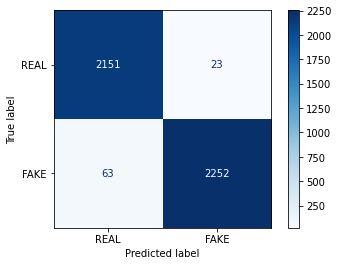
\includegraphics[width=1 \textwidth]{cnn-isot-cm}
		\end{subfigure}
		& 
		\begin{subfigure}{0.33\textwidth}
			\centering
			\caption{برت + پیچشی}
			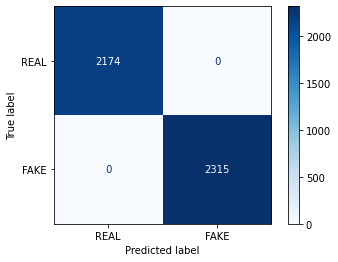
\includegraphics[width=1 \textwidth]{bert-cnn-isot-cm}
		\end{subfigure}
		&
		\begin{subfigure}{0.33\textwidth}
			\centering
			\caption{برت + پرسپترون ساده}
			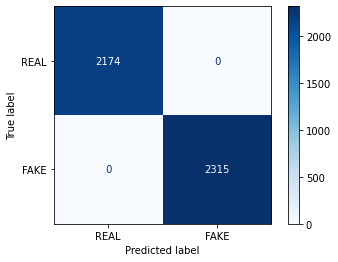
\includegraphics[width=1 \textwidth]{bert-slp-isot-cm}
		\end{subfigure}
	\end{tabular}
	\caption{ماتریس درهم‌ریختگی نتایج آزمایش‌های دادگان آی.اس.اُ.تی.}
	\label{ISOT-CM}
\end{figure}



همان‌طورکه از نتایج ارائه‌شده بر روی دادگان لیار و آی.اس.اُ.تی مشخص است، هر دو مدل «برت +‌ پرسپترون ساده» و «برت + پیچشی» نتایج قابل قبولی نسبت‌به روش‌های پیشین ارائه داده‌است. استفاده از لایه‌های پیچشی پس‌از بازنمایی ارائه شده توسط مدل برت به‌منظور به‌دست‌آوردن بازنمایی سطح بالاتر باتوجه‌به هم‌نشینی واژه‌ها در جمله بوده‌است؛ اما طبق نتایج به‌دست‌آمده توسط مدل پرسپترون ساده، بازنمایی‌های حاصل از مدل برت به میزان قابل قبولی دارای ویژگی‌های مناسبی برای نمایندگی واژه‌ها و جملات است. علاوه‌بر این، از مقایسه مدل «برت +‌ پیچشی» و مدل «ورد۲وک + پیچشی» که تنها از بازنمایی حاصل از همنشینی واژگان استفاده می‌کند، می‌توان نتیجه گرفت که قدرت مدل‌های ارائه‌شده در این بخش از پروژه حاصل از توانایی زیاد مدل برت برای بازنمایی جملات و کلمات است.

%7)
\chapter{بهبود تشخیص اخبار جعلی با فراداده‌های حاصل از پردازش زبان}
\section{انگیزه}
در بسیاری از موارد  صحت‌سنجی یک خبر با استفاده از متن خبر کار بسیار دشوار و پیچیده‌ای است. اما بعضی‌از فراداده‌های مرتبط با اخبار می‌تواند در تشخیص صحت این دسته از اخبار به ما کمک کند. در این فاز، به بررسی تأثیر استفاده از سه فراداده موضوع خبر، احساس خبر و موجودیت‌های نامدار موجود در خبر می‌پردازیم. با تحلیل و بررسی اخبار جعلی می‌توانیم دریابیم که آیا بعضی از موضوعات مثلاً سیاسی یا اجتماعی نسبت ‌به موضوعات دیگر مانند ورزشی بیشتر در معرض جعل خبر قرار دارد و خبر جعلی بیشتر در این موضوع مشخص تولید می‌شود یا خیر. دلیل این موضوع را می‌توان به‌دلیل تأثیرگذاری زیاد اخبار سیاسی و اجتماعی مطرح کرد. در صورت تأیید این فرضیه، انتظار می‌رود با دانستن موضوع هر خبر، بتوانیم درکنار متن خبر، با دقت بیشتری میزان جعلی‌بودن آن خبر را مشخص کنیم. علاوه بر این، یافتن موجودیت‌های نامدار و حس متن در هر خبر نیز می‌تواند اطلاعات نسبتاً مناسبی در مورد میزان صحت آن خبر ارائه دهد. در صورت تأیید این فرضیه نیز می‌توان حدس زد وجود اسامی خاص افراد، سازمان‌ها، مکان‌ها و ... در متن و یا حس مثبت یا منفی در متن می‌تواند به تشخیص جعلی‌بودن آن کمک کند. در ادامه این فصل به پردازش‌های متنی داده‌های خبری شامل دسته‌بندی موضوعی، تشخیص موجودیت‌های نامدار و تحلیل احساسات می‌پردازیم و در نهایت تأثیر آن‌ها را بررسی می‌نماییم.

\section{دسته‌بندی موضوعی اخبار}
\label{section.cat_detail}
همانطور که در بخش \ref{section.cat} به‌طور مفصل درمورد استخراج موضوع اخبار گفته شد، دو رویکرد اصلی برای استخراج موضوعات اخبار وجود دارد که ما بتوانیم با استفاده از آن‌ها دقت تشخیص اخبار جعلی را بالاتر ببریم. رویکرد اول استفاده از دسته‌بندی با مربی براساس ۶ کلاس مختلف است. در این حالت ما با استفاده از یک مدل آموزش‌دیده‌شده با پیکره بزرگ همشهری \citep{aleahmad2009hamshahri}، اخبار موجود در مجموعه دادگان «تاج» را برچسب می‌زنیم و از این برچسب به‌عنوان یک ویژگی جدا به‌صورت یک بردار ۶ بعدی در کنار ویژگی‌های مرتبط با متن مورد استفاده قرار می‌دهیم. رویکرد دوم استفاده از یک روش دسته‌بندی موضوعی بدون مربی 
	براساس روش تخصیص نهان دیریکله\LTRfootnote{Latent Dirichlet Allocation} \citep{blei2003latent} می‌باشد. 
	
در این روش یک بردار 50 بعدی که نماینده احتمال تعلق به هر موضوع است در کنار ویژگی‌های متنی آن برای تشخیص جعلی‌بودن خبر استفاده می‌شود.

\section{تشخیص موجودیت‌های نامدار}
شناسایی موجودیت­‌های نامدار در پردازش زبان طبیعی به عملیاتی گفته می‌­شود که در آن تمامی­ اسامی خاص موجود در متن شناسایی و استخراج می‌گردد و به مقولات ازپیش ‌تعریف‌شده‌ای مانند اسم افراد، سازمان‌ها، مکان‌ها و ... دسته بندی می‌شود به این صورت که متن را بر اساس واژه‌ها قطعه‌بندی نموده و با برچسب‌زنی، عبارات حاوی موجودیت‌های نامدار را مشخص می‌نماییم.

در واقع مسأله تشخیص موجودیت‌های نامدار در متن عموماً به دو زیر‌مسأله تشخیص و دسته‌بندی موجودیت‌ها تقسیم می‌شود. اسامی خاصی که تشخیص داده می‌شود و همچنین قالبی که برای دسته‌بندی آن‌ها به‌کار می‌رود وابسته به نوع کاربرد آن خواهد‌ بود. در سامانه‌های تشخیص موجودیت‌های نامدار، بیشتر بر روی تشخیص اسامی اشخاص، مکان‌­ها و سازمان‌هایی که در یک متن ذکر شده‌است تمرکز است \citep{chen2015}.

نیاز به شناسایی موجودیت­‌های نامدار در دنیای امروز که عصر ارتباطات و اطلاعات است به‌شدت احساس می‌­شود. شناسایی موجودیت‌­های نامدار برای جستجوهای معنادار\LTRfootnote{Semantic Search}، ترجمه ماشینی\LTRfootnote{Machine Translation}، استخراج اطلاعات از متن\LTRfootnote{Information Extraction}، مرجع‌یابی در متن\LTRfootnote{Co-reference Resolution}، سیستم­‌های پرسش و پاسخ\LTRfootnote{Question Answering Systems} ، سیستم‌های خبره\LTRfootnote{Expert Systems} ، کشف دانش\LTRfootnote{Knowledge Discovery} ، مدیریت دانش\LTRfootnote{Knowledge Management}، تحلیل احساسات\LTRfootnote{Sentiment Analysis}، بازیابی اطلاعات\LTRfootnote{Information Retrieval}، تحلیل خبر\LTRfootnote{News Analysis} و بسیاری دیگر از شاخه های مرتبط با پردازش زبان­ طبیعی کاربرد دارد. اینکه سیستم چه نوع موجودیتی را تشخیص دهد و یا به بیان دیگر دسته‌های معنایی مورد نظرش چه باشند، وابسته به زمینه کاربردی سیستم است \citep{ABDALLAH201734}.\\
به‌عنوان مثال، شناسایی موجودیت‌های نامدار در علم زیست‌شناسی می‌­تواند تشخیص اسامی وابسته به انواع پروتئین­، دی‌ان‌­ای، نوع سلول و غیره باشد. در حوزه پزشکی می‌تواند تشخیص انواع بیماری، دارو، و مراکز درمانی باشد. در حوزه تجارت نام شرکت‌­ها و مؤسسات، تراکنش­‌های مالی، بورس و غیره باشد؛ یا به‌صورت خیلی خاص  تنها برای تشخیص اسامی شرکت­‌های تولید کننده فولاد به‌کار رود.

یکی از کاربردهای تشخیص موجودیت‌­های نامدار در ترجمه ماشینی رفع ابهام از ترجمه و افزایش دقت آن است. به‌عنوان مثال، اگر در متنی واژه \lr{Apple} به‌عنوان موجودیت نامدار شناخته شده باشد و دارای برچسب باشد، در این صورت در هنگام ترجمه به‌عنوان شرکت «اپل» شناخته می‌­شود و معنای «سیب» نخواهد داشت. در مثالی دیگر، در ترجمه فارسی به انگلیسی می‌­توان به واژه «زیبا» اشاره کرد. اگر این واژه اسم فرد و موجودیت نامدار باشد، نیاز به ترجمه ندارد، و درغیراین‌­صورت باید به واژه \lr{Beautiful} ترجمه شود \citep{Hussain2016}.

به طور کلی از دو روش قاعده‌مند و آماری برای تشخیص موجودیت‌­های نامدار استفاده می‌­شود \citep{Jurafsky2009}. در روش‌­های قاعده‌مند، قوانینی تعریف می‌­شود که براساس آنها موجودیت‌­های نامدار تشخیص داده می‌­شود. در روش آماری، از تکنیک­‌های یادگیری ماشین برای دسته­‌بندی موجودیت­‌های نامدار به هر مقوله استفاده می‌­شود. استفاده از روش­‌های دسته‌بندی بانظارت در این قسمت سبب می‌­شود  با استفاده از پیکره‌هایی که موجودیت‌­های نامدار  در آن‌ها برچسب‌گذاری شده‌است  مدلی را آموزش داد، و با استفاده از آن مدل بتوان متن بدون برچسب را برچسب‌گذاری نمود و موجودیت‌های نامدار را در آن‌ها به‌طور خودکار تشخیص داد. در پروژه حاضر، برای ساخت سامانه تشخیص موجودیت­‌های نامدار از روش­‌های یادگیری ماشین بانظارت و مبتنی ‌بر یادگیری عمیق استفاده می‌کنیم.

\subsection{دادگان}
برای یادگیری مدل، نیازمند پیکره‌­ای برای آموزش شبکه عصبی هستیم. از جمله دادگان موجود در زمینه تشخیص موجودیت­‌های نامدار در زبان فارسی، پیکره‌های موجویت‌­های نامدار آرمان \citep{poostchi2016personer}، پیما \citep{shahshahani2019peyma} و درخت‌بانک هسته‌بنیان فارسی \citep{ghayoomi2012} می‌­باشد. در پیکره سوم  تنها موجودیت‌­های نامدار مربوط به نام اشخاص، موقعیت­‌های مکانی و اسامی مربوط به سازمان‌­ها برچسب‌گذاری شده‌است. درحالی‌که در پیکره اول، علاوه‌بر این سه برچسب، اسامی رویدادها، امکانات و محصولات نیز مشخص شده و در پیکره دوم نیز زمان، تاریخ، مبالغ مالی و درصد برچسب‌گذاری شده‌است.  این در حالی است که در بسیاری از کاربردهای تشخیص موجودیت‌­های نامدار، مانند سیستم‌­های پرسش و پاسخ و یا تحلیل اخبار و ...، نیازمند پوشش موجودیت­‌های نامدار بیشتری مانند زبان‌­ها، ملیت‌­ها، رخدادها، مشاغل، کتاب‌­ها، اسامی فیلم‌­ها، تاریخ­‌ها، مذاهب، زمینه‌های علمی و دانش‌­ها، روزنامه‌­ها و سایر اسامی خاص در زبان هستیم.

ازآنجاکه در پیکره­‌های مذکور این موارد پوشش داده نشده بود، برای به‌کاربردن ویژگی‌های حاصل از تشخیص موجودیت­‌های نامدار در تشخیص اخبار جعلی، از پیکره‌­ موجودیت‌های نامدار تهیه‌شده در آزمایشگاه پردازش زبان طبیعی دانشگاه صنعتی امیرکبیر که حاوی پانزده برچسب موجودیت‌­های نامدار است استفاده شده‌است \citep{momtazi2020named}. این دادگان که شامل حدود ۳۰۰۰ چکیده ویکی‌پدیا بوده و به‌صورت دستی برچسب‌خورده است می‌­تواند در این پژوهش مورد استفاده قرار بگیرد و سبب شود تجزیه­ و­ تحلیل و نتیجه‌گیری از داده‌ها را با دقت بالاتری انجام دهد. 

در ادامه، به توضیح اجمالی برچسب‌های این پیکره می‌پردازیم. واژه‌ها گردآوری‌شده از ویکی‌پدیای فارسی برای آموزش سیستم نیازمند برچسب‌گذاری با نمادهایی است که هر کدام به یک نوع از موجودیت‌­های نامدار اشاره دارد. تعداد کل برچسب­‌های استفاده‌شده در دادگان ۳۱ برچسب است که برای مشخص‌کردن ۱۵ نوع موجودیت متفاوت که شامل اسم شخص مفرد، اسم شخص جمع، موقعیت مکانی، اسم سازمان، زبان، ملیت، رخداد، شغل، کتاب، اسم فیلم، تاریخ، مذهب، عنوان علمی و دانش، روزنامه و سایر اسامی خاص ذکرنشده در زبان فارسی می‌باشد استفاده شده‌است. همچنین برای واژه‌هایی که جزو موجودیت­‌های نامدار نیست نیز علامتی در نظر گرفته شده‌است. در این دادگان، برای تعیین اسم خاص اشخاص از دو برچسب مختلف استفاده شده‌است که یکی برای تعیین اسامی خاص مفرد و معمول به‌کار می‌­رود و با علامت \lr{PEI} مشخص شده و دیگری برای اسامی خاص که به‌صورت جمع استفاده می‌شود کاربرد دارد. این موارد با برچسب \lr{PEG} مشخص شده‌است.

اسم شخص جمع به تمامی اسامی گفته می‌شود که اسم مفرد آن نوعی موجودیت باشد. به‌­عنوان مثال واژه‌های «مسلمان»، «معلم» و «ایرانی» به‌­ترتیب برچسب‌­های مذهب، شغل و ملیت می‌­گیرند و اسم جمع این واژه‌ها یعنی «مسلمانان»، «معلمان» و «ایرانیان» \lr{PEG} محسوب می‌­شود. همین‌طور واژه «ابوالفضل بلعمی» دارای برچسب \lr{PEI} است و به طبع آن واژه‌های «خاندان بلعمی» و یا «بلعمیان» برچسب \lr{PEG} دارد. جدول \ref{table.NER_tags} به تفضیل به شرح و بررسی برچسب­‌های استفاده‌شده برای دادگان می‌پردازد.

\begin{table}
	\caption{راهنمای برچسب واژگان}
	\label{table.NER_tags}
	\begin{center}
		\small
		\begin{tabular}{|P{1.2cm}|P{2cm}|P{2cm}|P{8cm}|}
			\hline
			برچسب & تعریف انگلیسی برچسب & تعریف فارسی برچسب & توضیحات \\
			\hline
			\lr{O} & \lr{Out} &
			هیچ & واژه مورد نظر از موجودیت‌های نامدار نیست. \\
			\hline
			\lr{PEI} & \lr{Person Individual} &
			شخص مفرد & این علامت به نام شخص اشاره دارد. \\
			\hline
			\lr{PEG} & \lr{Person Group} &
			اسم خاص گروه & این علامت به موجودیت نامداری اشاره دارد که به‌صورت جمع آمده‌است.\\
			\hline
			\lr{LOC} & \lr{Location} &
			موقعیت مکانی & واژه مورد نظر این برچسب به موقعیت مکانی خاصی اشاره دارد. \\
			\hline
			\lr{ORG} & \lr{Organization} &
			سازمان  & اسامی سازمان‌­ها و مؤسسات مختلف با این برچسب نشان داده می‌­شود. \\
			\hline
			\lr{LAN} & \lr{Language} &
			زبان & این برچسب نشان‌دهنده زبان‌­های مختلف است. \\
			\hline
			\lr{NAT} & \lr{Nationality} &
			ملیت & ملیت­‌های مختلف با این علامت تعیین می‌­شود. \\
			\hline
			\lr{EVN} & \lr{Events} &
			رخدادها & رخدادها و وقایع خاص را با این برچسب نشان دادیم. \\
			\hline
			\lr{JOB} & \lr{Job} &
			شغل & این برچسب نمایانگر مشاغل است. \\
			\hline
			\lr{BOK} & \lr{Book} &
			کتاب & اسامی کتاب‌­ها با این برچسب مشخص می‌شود. \\
			\hline
			\lr{FLM} & \lr{Film} &
			فیلم & نام فیلم‌­های مختلف با این برچسب تعیین می‌­شود. \\
			\hline
			\lr{DTE} & \lr{Date} &
			تاریخ & برای نشان‌دادن تاریخ و دوره‌های مختلف از برچسب استفاده شده‌است. \\
			\hline
			\lr{REL} & \lr{Religion} &
			مذهب & این برچسب تعیین‌کننده مذاهب مختلف است. \\
			\hline
			\lr{FLD} & \lr{Field} &
			زمینه & زمینه‌ها و دانش‌­های مختلف با این برچسب تعیین گردیده‌است. \\
			\hline
			\lr{MAG} & \lr{Magazine} &
			روزنامه و مجله & اسامی روزنامه‌ها و مجلات با این برچسب آمده‌است. \\
			\hline
			\lr{OTH} & \lr{Other} &
			سایرین & اگر واژه‌ای به‌عنوان موجودیت نامدار باشد ولی در بین موجودیت­‌های معرفی‌شده در بالا نباشد با این برچسب مشخص می‌­شود. \\
			\hline
			
		\end{tabular}
	\end{center}
\end{table}

\subsection{مدل}
اساس خیلی از برنامه‌ها قابلیت پیش‌بینی دنباله‌ای از متغیر‌ها است که به همدیگر وابسته هستند. این مسئله کاربرد زیادی در حوزه‌های مختلف پردازش متن دارد. برای تشخیص موجودیت‌های نامدار باید دنباله واژه‌ها را مدل کرد و برای هر واژه یک خروجی ساخت. برای مدل‌سازی دنباله‌ها روش‌های متعددی وجود دارد که در این میان رویکرد مبتنی‌بر شبکه عصبی بازگشتی با میدان شرطی تصادفی بیشترین محبوبیت را دارد. این مدل یک شبکه عصبی بازگشتی دوطرفه به‌‌علاوه یک لایه میدان تصادفی شرطی در انتها است. شبکه عصبی بازگشتی برای یک واژه اطلاعاتی در مورد بافت آن واژه و واژه‌ها قبل از آن مهیا می‌کند و در حالت دوطرفه علاوه بر واژه‌های قبل، واژه‌های بعد از آن را هم در نظر می‌گیرد. لایه میدان تصادفی شرطی برای پیش‌بینی برچسب هر واژه، برچسب واژه‌های دیگر را نیز در نظر می‌گیرد.

مشابه رویکردی که در بازنمایی متون در تشخیص اخبار جعلی داشتیم در بخش تشخیص موجودیت‌های نامدار نیز بازنمایی عصبی با استفاده از مدل‌های زبانی مبتنی بر معماری انتقال‌دهنده‌ مورد استفاده قرار گرفته است. برت می‌تواند برای طیف گسترده‌ای از کارهای زبانی مورد استفاده قرار گیرد‌، در حالی که فقط یک لایه به مدل اصلی اضافه می‌شود. در تشخیص موجودیت‌های نامدار‌ با استفاده از برت می‌توان با تغذیه بردار خروجی هر نشانه در یک لایه طبقه‌بندی که برچسب موجودیت نامدار را پیش‌بینی می‌کند‌، یک مدل تشخیص موجودیت نامدار آموزش داد.

اگرچه مدل حاصل از ترکیب شبکه عصبی بازگشتی و میدان شرطی تصادفی در پژوهش‌های مختلف به نتایج بهتری نسبت‌به مدل‌های قبلی رسیده‌است \citep{huang2015bidirectional}، با استفاده از مدل‌های مبتنی‌بر ترانسفورمر برای بازنمایی متن ویژگی‌های مورد استفاده در شبکه \lr{BiLSTM} در بخش بازنمایی مورد توجه قرار می‌گیرد و استفاده از شبکه \lr{BiLSTM} پس‌از بازنمایی به دقت مدل نمی‌افزاید \citep{Thesis_abdolah}. در نتیجه، در پژوهش حاضر برای تشخیص موجودیت‌های نامدار از شبکه برت به‌همراه یک لایه میدان شرطی تصادفی استفاده می‌کنیم. 

درمیان مدل‌های مبتنی‌بر برت که برای زبان فارسی قابل استفاده است، مدل ایکس.ال.ام-روبرتا به نتایج قابل قبولی در این زمینه رسیده‌است و براساس نتایج گزارش‌شده توسط \cite{Thesis_abdolah} از این مدل برای تشخیص موجودیت نامدار استفاده می‌شود.

\section{تحلیل احساسات}
نظرکاوی یا تحلیل احساسات، مطالعه محاسباتی نظرات کاربران حول محصولات، خدمات، سازمان‌ها، اشخاص، رویدادها و جنبه‌های مختلف آن است. در سال‌های اخیر این حوزه یکی از حوزه‌های پژوهشی فعال در پردازش زبان‌های طبیعی بوده است. نظرکاوی در سطوح مختلف سند، جمله و جنبه مورد مطالعه قرار گرفته‌است. در حوزه کالا و خدمات هنگام تصمیم‌گیری عقاید دیگران تأثیر به‌سزایی در تصمیم نهایی دارد. در دنیای واقعی، شرکت‌ها همواره نیازمند عقاید مردم برای بهبود کیفیت و توسعه خدمات خود است. در دنیای نشر خبر، سوگیری احساسی اخبار یکی از جنبه‌های مؤثر در تحلیل خبر می‌باشد. مثبت یا منفی بودن یک خبر می‌تواند جنبه‌های مختلفی از تحلیل آن خبر را فراهم آورد. درحال‌حاضر داده‌های متنی  بخش عظیمی از شبکه‌های اجتماعی، فروشگاهای اینترنتی و انواع مختلف سامانه‌های ارتباطی را در بر گرفته‌است. از این داده‌ها می‌توان در راستای درک احساسات کاربران به مطالب مختلف مانند یک محصول، یک نوشته موضوعی و ... استفاده کرد. 

نظر‌کاوی در سال 2002 توسط \citet{pang2002} معرفی شد. با روی‌کارآمدن شبکه‌های اجتماعی و تأثیر روزافزون آن‌ها بر زندگی مردم، اهمیت نظر‌کاوی و کاربردهای آن بیشتر مشخص گردید. باتوجه‌به این که افراد با حضور در این شبکه‌ها به بیان نظرات، عقاید و دیدگاه‌های خود درباره کلیه مسائل سیاسی، اجتماعی، فرهنگی، اقتصادی و حتی فردی می‌پردازد، تحلیل احساسات بیشتر از هر چیز در شبکه‌های اجتماعی مورد توجه قرار گرفته‌است. در کنار بستری که در شبکه‌های اجتماعی فراهم شده‌است، متون موجود در داده‌های خبری نیز می‌توانند دارای حس مثبت یا منفی باشد که به تحلیل آن کمک می‌نماید.

برای استفاده از تحلیل احساسات در تشخیص اخبار جعلی، تحلیل احساس در سطح سند مورد توجه این پژوهش قرار گرفته‌است و با بهره‌گیری از یک مدل مبتنی‌بر یادگیری عمیق حس موجود در متن به‌صورت یک بردار دو بعدی برای حس مثبت و منفی مشخص می‌گردد. خروجی این مدل به‌عنوان یکی از ویژگی‌های ورودی در مدل تشخیص اخبار جعلی استفاده خواهد شد.

\subsection{مدل}
برای پیاده‌سازی بخش تشخیص احساسات از شبکه پیچشی استفاده شده‌است. باتوجه‌ به این که پایه اصلی تحلیل احساسات دسته‌بندی متون است، ساختار شبکه پیچشی مورد استفاده در این بخش مشابه شبکه پیچشی‌ای است که در تشخیص خبر جعلی مورد استفاده قرار گرفته‌است و توضیحات آن در بخش ۳-۲-۲ گزارش فاز اول آمده‌است.  بازنمایی مورد استفاده در این شبکه نیز بازنمایی ایکس.ال.ام-روبرتا می‌باشد.

\section{نتایج حاصل از استفاده از پردازش‌های متنی در تشخیص اخبار}
در فصل ۳، با بررسی و مقایسه مدل‌های از پیش آموزش دیده، بهترین مدل بازنمایی اخبار ورودی را انتخاب کردیم. در این بخش می‌خواهیم با استفاده از هر دو مدل دسته‌بند شبکه پیشرو پرسپترون و شبکه عصبی پیچشی و استفاده از مدل پارس‌برت برای بازنمایی اخبار، از فراداده‌هایی مانند موضوع خبر، موجودیت‌های نامدار و یا حس متن در کنار بردار بازنمایی متن خبر استفاده کنیم.

همانطور که در بخش \ref{section.cat_detail} گفته شد برای استفاده از ویژگی موضوع خبر در رویکرد اول  یک بردار ویژگی ۶ بعدی حاصل از دسته‌بندی موضوعی اخبار و در رویکرد دوم یک بردار ویژگی ۵۰ بعدی حاصل از تخصیص نهان دیریکله خواهیم داشت. بازنمایی خروجی تحلیل احساس نیز یک بردار دو بعدی است که هر درایه آن نشان‌دهنده مثبت و یا منفی بودن آن خبر است. همچنین، اطلاعات مربوط به موجودیت‌های نامدار موجود در یک خبر با استفاده از یک بردار شامل ۱۵ ویژگی بازنمایی می‌شود. برای نمونه،  در جدول \ref{table.ner_example} نمونه‌ای از یک جمله برچسب‌گذاری‌شده نمایش داده شده‌است. در بردار ۱۵تایی حاصل از این جمله، درایه مربوط به موجودیت کتاب مقدار ۲، درایه‌های مربوط به موجودیت‌های زبان، شخص مفرد، شغل و تاریخ مقدار ۱، و سایر درایه‌ها مقدار صفر خواهد داشت. 
\begin{table}[h!]
	\caption{مثال از یک جمله برچسب‌خورده توسط مدل تشخیص موجودیت نامدار}
	\label{table.ner_example}
	\begin{center}
		\begin{tabular}{|c|c|}
			\hline
			واژه & برچسب \\
			\hline
			\hline
			کتاب &\lr{b-BOK} \\
			گلستان & \lr{i-BOK} \\
			و & \lr{O} \\
			کتاب & \lr{b-BOK} \\
			بوستان & \lr{i-BOK} \\
			از & \lr{O} \\
			شاهکارهای & \lr{O} \\
			ادب & \lr{O} \\
			فارسی & \lr{b-LAN} \\
			و & \lr{O} \\
			اثر & \lr{O} \\
			سعدی & \lr{b-PEI} \\
			شاعر & \lr{b-JOB} \\
			قرن & \lr{b-DTE} \\
			ششم & \lr{i-DTE} \\
			هجری & \lr{i-DTE} \\
			است & \lr{O} \\
			\hline
			
		\end{tabular}
	\end{center}
\end{table}


به‌منظور استفاده از ویژگی‌های فراداده‌های مختلف،  بردار‌های این ویژگی‌ها را ابتدا به یک لایه چگال با همان تعداد نورون وارد می‌کنیم و پس‌از‌ آن بردار خروجی لایه چگال را به انتهای بردار ویژگی‌های نهایی استخراج‌شده از متن اخبار الحاق می‌کنیم. درنهایت پس‌ از ساخت بردار ویژگی جدید، شامل ویژگی‌های متن و فراداده‌ها، آن را وارد یک لایه پرسپترون می‌کنیم تا برچسب اخبار مشخص شود. شِمای کلی مدل ارائه‌شده برای استفاده از تمام فراداده‌ها در کنار ویژگی‌های مبتنی بر بافت اخبار در شکل \ref{fig.all_features} ارائه شده است. همچنین، شکل \ref{fig.cnn_ner}  معماری شبکه عصبی پیچشی را در حالت استفاده از بردار فراداده‌ها نشان می‌دهد. 

\begin{figure}[h!]
	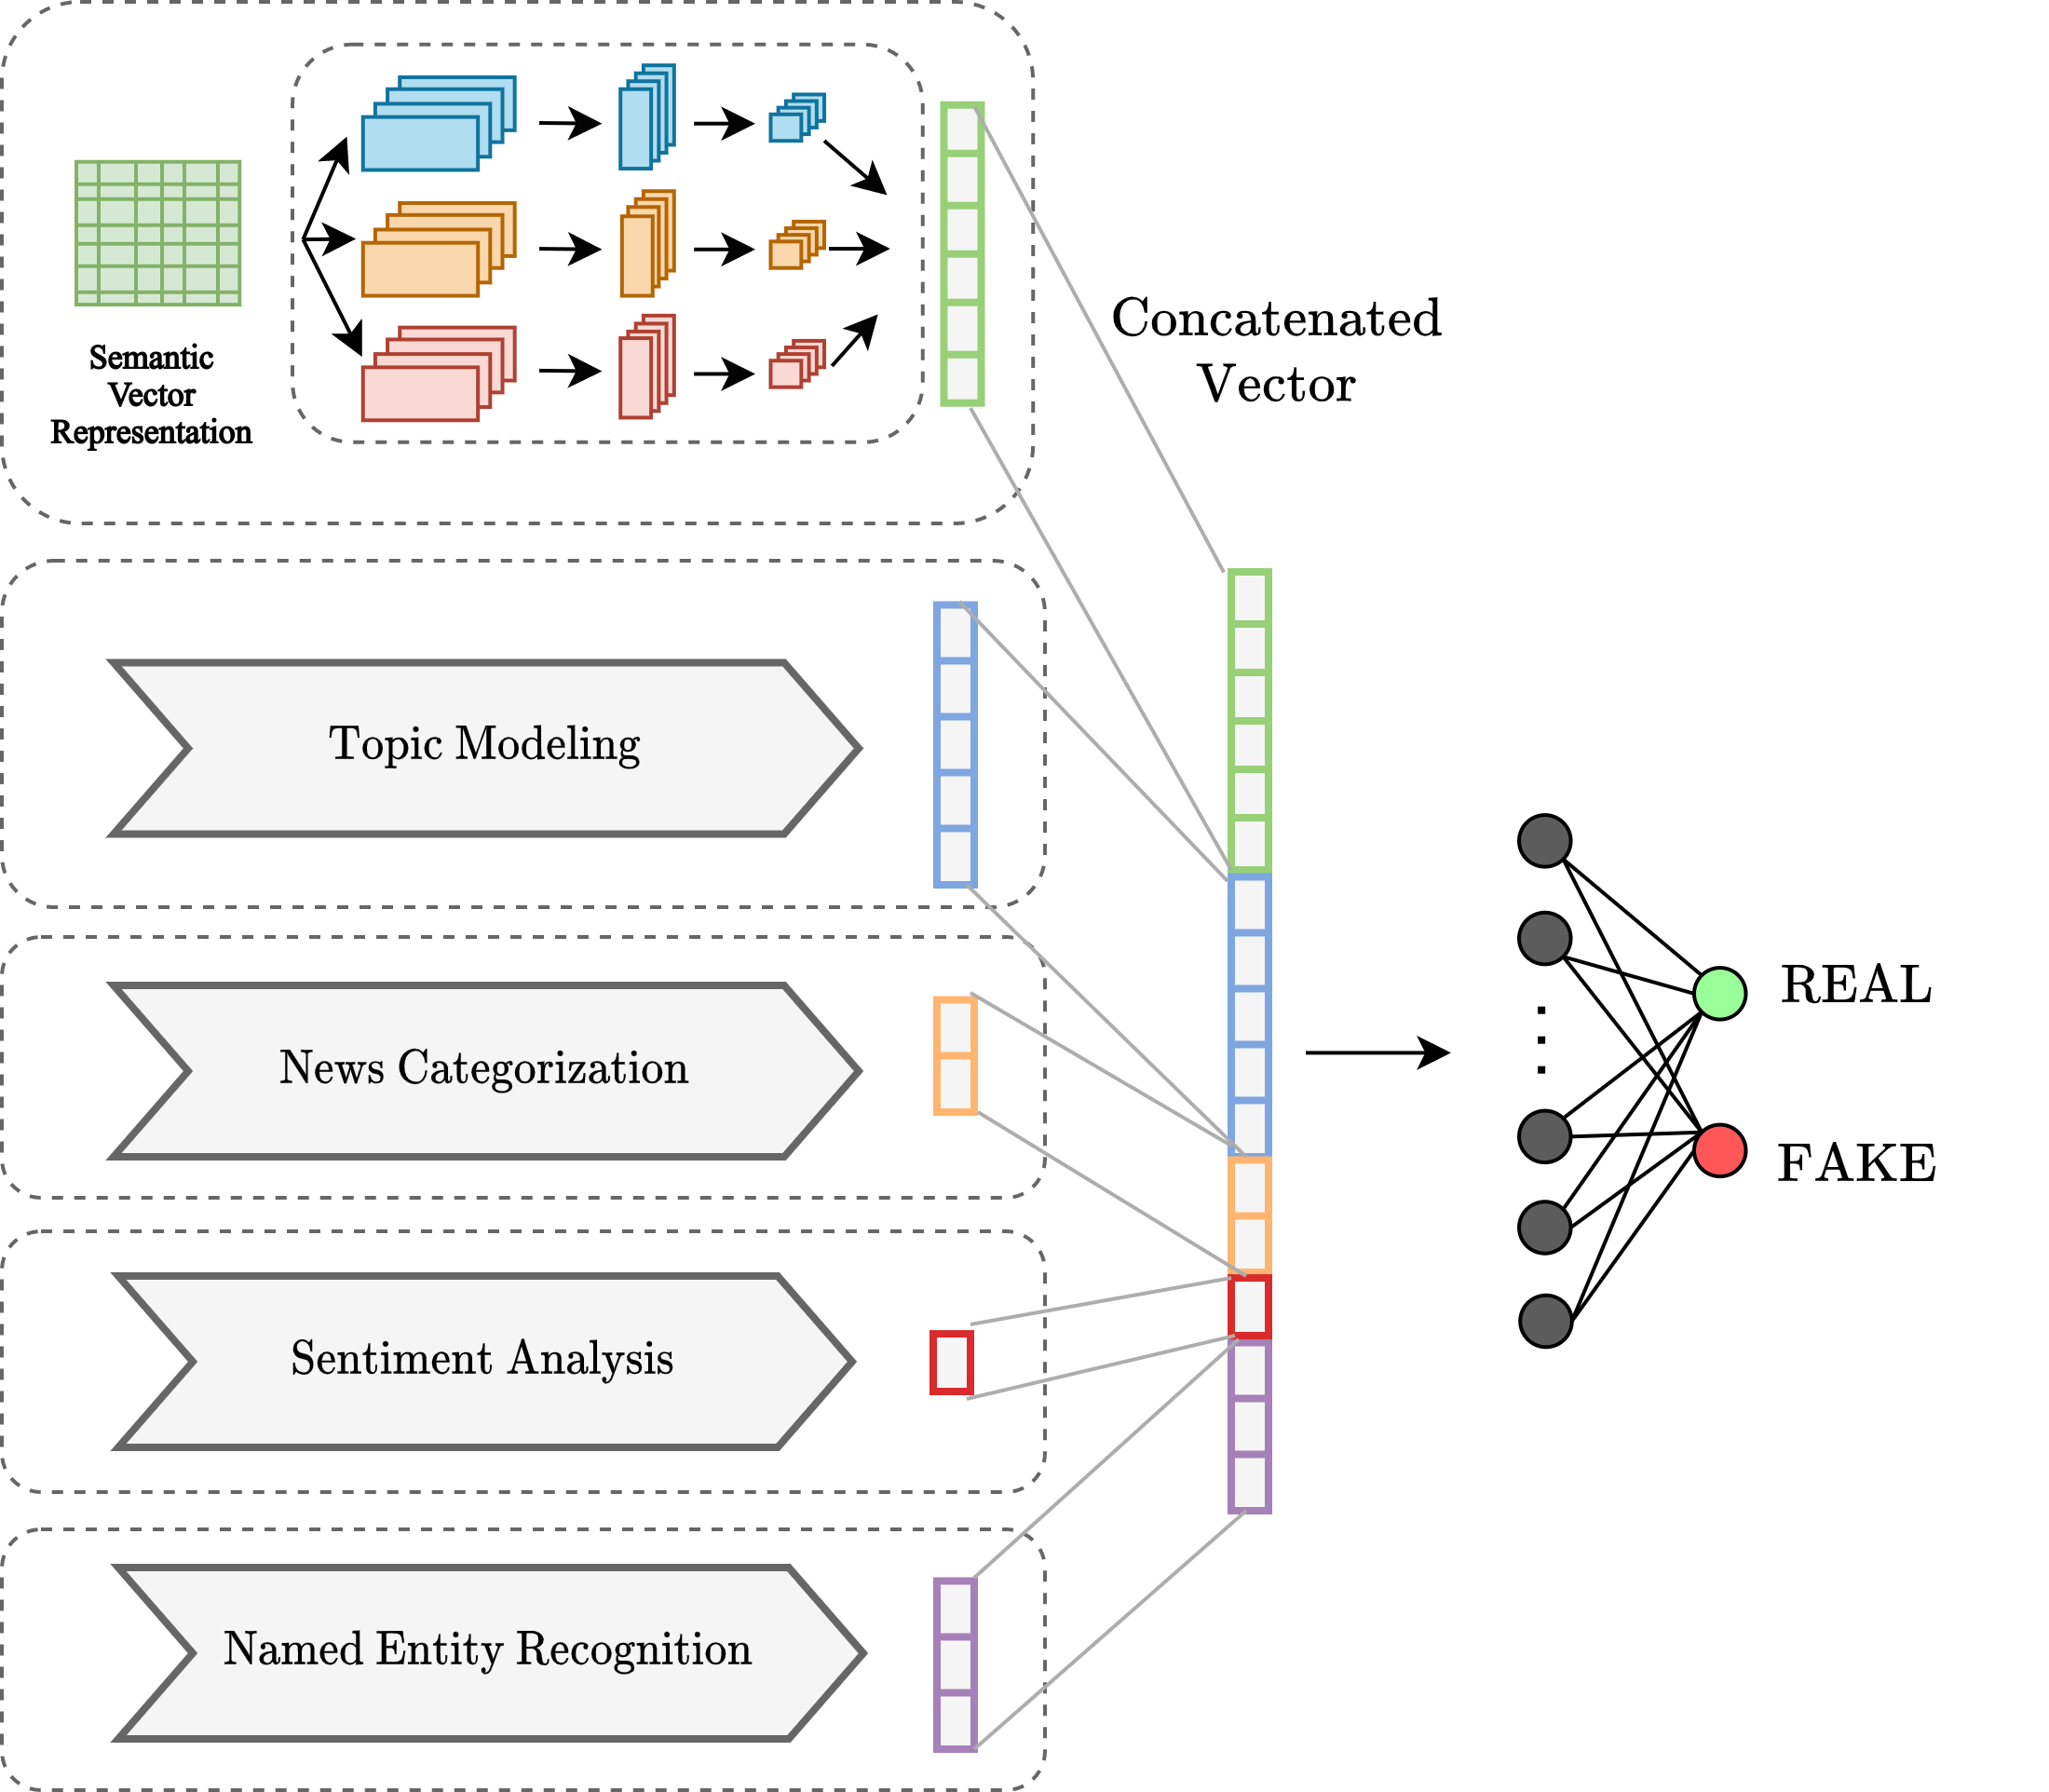
\includegraphics[width=0.75 \textwidth]{all_features}
	\centering
	\caption{شمای کلی مدل استفاده شده برای استفاده از تمام فراداده‌ها}
	\label{fig.all_features}
\end{figure}

\begin{figure}[h!]
	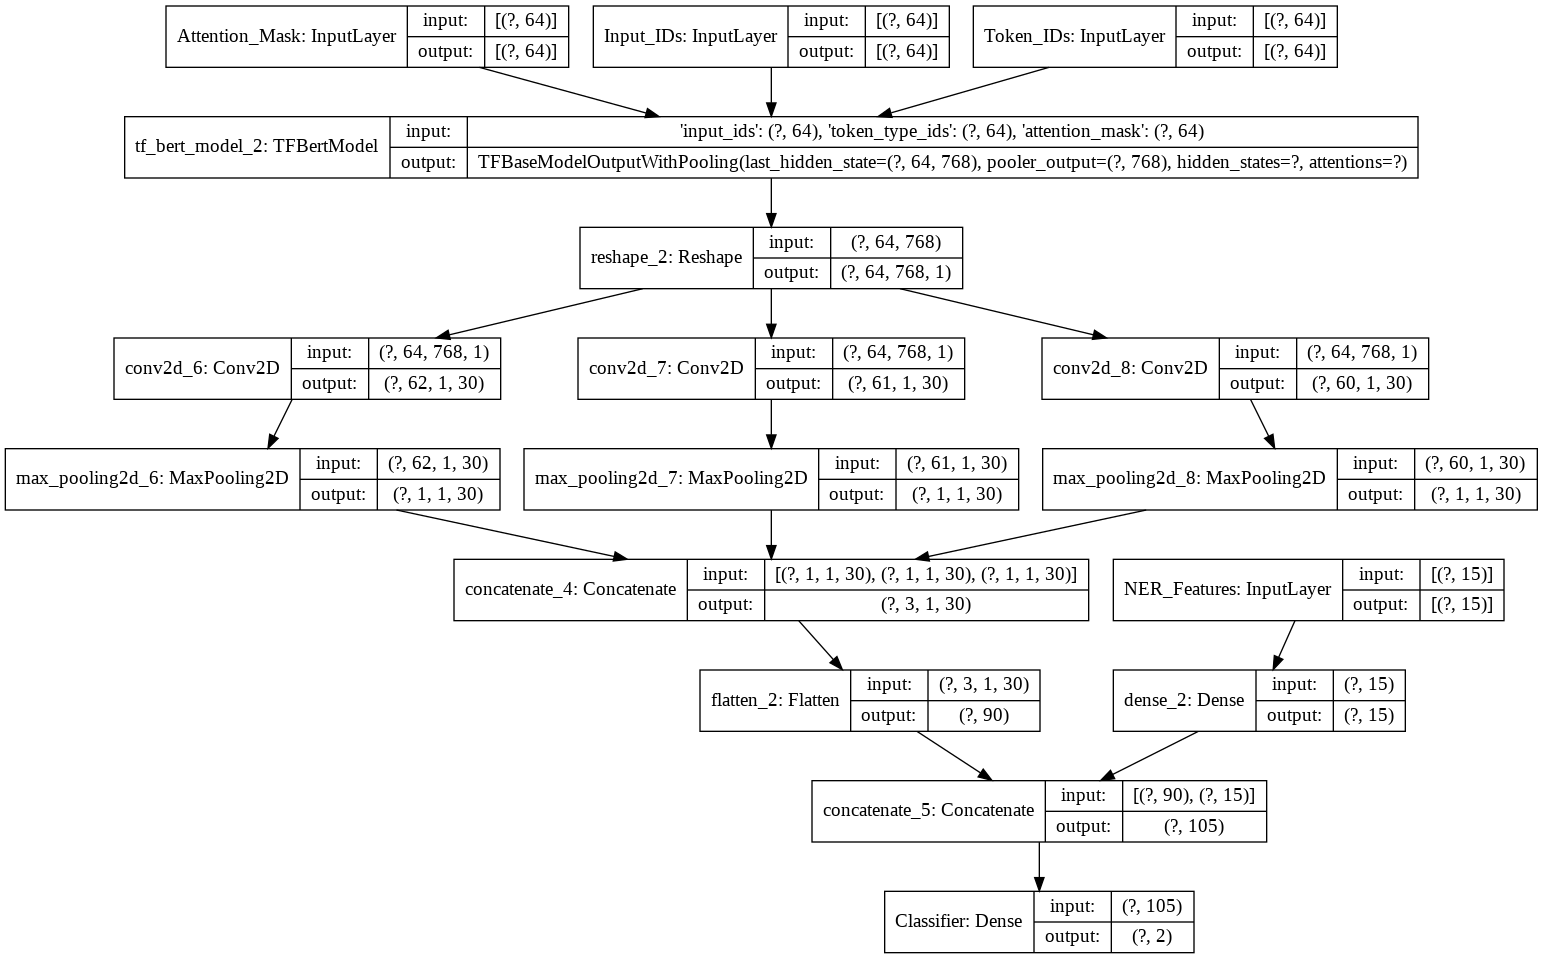
\includegraphics[width=1 \textwidth]{model_cnn_ner}
	\centering
	\caption{معماری مدل پیچشی با استفاده از فراداده موجودیت‌های نامدار}
	\label{fig.cnn_ner}
\end{figure}

جدول \ref{table.results_meta} نتایج حاصل از استفاده از هریک از فراداده‌های ذکرشده در کنار بازنمایی متنی  در دو شبکه پیچشی و پیشرو را نمایش می‌دهد. برای مقایسه راحت‌تر، نتایج حاصل از تشخیص اخبار بدون فراداده که در فصل قبل گزارش شده بود در این جدول تکرار شده‌است.
براساس جدول \ref{table.results_meta}، با استفاده از پردازش‌های متنی توانستیم دقت تشخیص اخبار جعلی را بهبود دهیم. همانطور که انتظار داشتیم دسته‌بند پیچشی توانست عملکرد بهتری را نسبت به مدل شبکه عصبی پرسپترون پیشرو داشته باشد. با توجه به نتایج، ازشمندترین فراداده که توانست دقت تشخیص مدل ما را بیشتر بهبود دهد، موضوع هر خبر (دسته‌بندی) بود که باعث افزایش \%$1.2$ معیار اف و \%$1.6$ دقت دسته‌بند پیچشی شد. این نتیجه دور از انتظار هم نبود چراکه موضوع هر خبر تاثیر بسیار زیادی در تشخیص اخبار جعلی دارد. همانطور که پیش از این هم اشاره شده، عمده اخبار جعلی در حوزه‌های سیاسی و اجتماعی منتشر می‌شوند. همچنین فراداده‌های مربوط به احساس‌ خبر، بردار موجودیت‌های نام‌د‌ار و موضوع (تخصیص نهان دیریکله) توانستند به طور مجزا دقت نهایی مدل را \%$0.5$، \%$1.35$ و \%$0.3$ افزایش دهند. در نهایت با استفاده از تمامی فراداده‌های استخراج شده از اخبار که با پیوستن به یکدیگر یک بردار ۷۳ بعدی را تشکیل دادند، مدل‌ پارس‌برت-پیچشی ارائه شده را ارزیابی کردیم که باعث افزایش ۲ درصدی معیار اف و دقت شد.

\begin{table}[h!]
	\caption{نتایج تشخیص اخبار جعلی فارسی با استفاده از بازنمایی پارس‌برت و دسته‌بندهای مختلف}
	\label{table.results_meta}
	\begin{center}
		\begin{tabular}{|c|c|c|c|c|c|c|}
			\hline
			بازنمائی & دسته‌بند & فراداده & فراخوانی & صحت & معیار اف & دقت \\
			\hline
			\hline
			\multirow{11}{*}{پارس‌برت} & \multirow{5}{*}{پیچشی}
			& - & $89.13$ & $93.71$ & $91.36$ & $91.64$ \\
			\cline{3-7}
			&  & موجودیت‌های نامدار & $91.16$& $94.28$ & $92.69$ & $92.99$ \\
		\cline{3-7}
			&  & احساس‌ خبر & $91.52$ & $92.57$ & $92.04$ & $92.45$ \\
			\cline{3-7}
			 &  & موضوع  (دسته‌بندی) & $96.87$ & $88.57$ & $92.53$ & $93.26$ \\
			\cline{3-7}
		 &  & موضوع  (تخصیص نهان دیریکله) & $91.42$ & $91.42$  & $91.42$  & $91.91$  \\
			\cline{3-7}
			&  & تمام ویژگی‌ها & $93.64$ & $92.57$ & $93.10$ & $93.53$ \\
			\cline{2-7}
			& \multirow{5}{*}{پرسپترون}
			& - & $92.44$ & $90.85$ & $91.64$ & $92.18$ \\
			\cline{3-7}
			&  &موجودیت‌های نامدار & $93.16$ & $85.71$ & $89.28$ & $90.29$ \\
			\cline{3-7}
			&  &احساس‌ خبر & $83.90$ & $98.28$ & $90.52 $ & $90.29$ \\
			\cline{3-7}
		&  & موضوع  (دسته‌بندی) & $89.13$ & $93.71$ & $91.36$ & $91.64$ \\
			\cline{3-7}
			&  & موضوع  (تخصیص نهان دیریکله)  & $87.89 $ & $95.42$ & $91.50$ & $91.64$ \\
			\hline
		\end{tabular}
	\end{center}
\end{table}
%8)
\chapter{جمع‌بندی و کارهای آتی}
در این گزارش شرح جمع‌آوری داده برای زبان انگلیسی و پیاده‌سازی روش پیشنهادی برای دادگان انگلیسی ارائه شده‌است. همچنین پیاده‌سازی‌های مقدماتی برای بازنمایی متون فارسی صورت شده‌است تا بتوان در گام بعد پس‌از برچسب‌زنی داده فارسی، دسته‌بندی متون فارسی را با استفاده از بازنمایی‌های ذکرشده به‌انجام رساند. در فاز دوم، مروری بر کارهای مرتبط با فارسی ارائه خواهد شد و سپس جمع‌آوری داده فارسی و برچسب‌زنی آن انجام خواهد شد. در فاز سوم نیز با استفاده از داده‌های تهیه‌شده سیستم تشخیص اخبار جعلی فارسی تهیه خواهد شد. درنهایت، در فاز چهارم به بهبود این سیستم و ارائه محصول پرداخت خواهد شد.

%--------------------------------------------------------------------------appendix( مراجع و پیوست ها)
\chapterfont{\vspace*{-2em}\centering\LARGE}%

\appendix
\bibliographystyle{chicago-fa}
\bibliography{references}
%\chapter*{‌پیوست}
\markboth{پیوست}{}
\addcontentsline{toc}{chapter}{پیوست}
موضوعات مرتبط با متن گزارش پایان نامه كه در يكی از گروه‌های زير قرار می‌گيرد، در بخش پيوست‌ها آورده شوند:
\begin{enumerate}
\item  اثبات های رياضی يا عمليات رياضی طولانی‌.‌
\item داده و اطلاعات نمونه (های) مورد مطالعه (\lr{Case Study}) چنانچه طولانی باشد‌.‌
\item نتايج كارهای ديگران چنانچه نياز به تفصيل باشد‌.‌
\item مجموعه تعاريف متغيرها و پارامترها، چنانچه طولانی بوده و در متن به انجام نرسيده باشد‌.‌
\end{enumerate}
% براي شماره‌گذاري روابط، جداول و اشكال موجود در پيوست‌ از ساختار متفاوتي نسبت به متن اصلي استفاده مي‌شود كه در زير به‌عنوان نمونه نمايش داده شده‌است. 
% \begin{equation}
%F=ma
%\end{equation}
\section*{کد میپل }
\begin{latin}
\begin{verbatim}

with(DifferentialGeometry):
with(Tensor):
DGsetup([x, y, z], M)
																	frame name: M
a := evalDG(D_x)
																	D_x
b := evalDG(-2 y z D_x+2 x D_y/z^3-D_z/z^2)


\end{verbatim}
\end{latin}
%--------------------------------------------------------------------------dictionary(واژه نامه ها)
%اگر مایل به داشتن صفحه واژه‌نامه نیستید، خط زیر را غیر فعال کنید.
%\parindent=0pt
%%
\chapter*{واژه‌نامه‌ی فارسی به انگلیسی}
\pagestyle{style9}

\addcontentsline{toc}{chapter}{واژه‌نامه‌ی فارسی به انگلیسی}
%%%%%%
\begin{multicols*}{2}

{\bf آ}
\vspace*{3mm}


\farsiTOenglish{اسکالر}{Scalar}


\vspace*{3mm}
{\bf ب}
\vspace*{3mm}

\farsiTOenglish{بالابر}{Lift}


\vspace*{3mm}
{\bf پ}
%%\vspace*{3mm}

\farsiTOenglish{پایا}{Invariant}



\vspace*{3mm}
{\bf ت}
%%\vspace*{3mm}

\farsiTOenglish{ تناظر }{Correspondence}


\vspace*{3mm}
{\bf ث}
%%\vspace*{3mm}

\farsiTOenglish{ثابت‌ساز}{Stabilizer}

\vspace*{3mm}
{\bf ج}
%%\vspace*{3mm}

\farsiTOenglish{جایگشت}{Permutation}



\vspace*{3mm}
{\bf چ}
%%\vspace*{3mm}


\farsiTOenglish{چند جمله‌ای }{Polynomial}

\vspace*{3mm}
{\bf ح}
%%\vspace*{3mm}

\farsiTOenglish{حاصل‌ضرب دکارتی}{Cartesian product}


\vspace*{3mm}
{\bf خ}
%%\vspace*{3mm}

\farsiTOenglish{خودریختی}{Automorphism}

\vspace*{3mm}
{\bf د}
%%\vspace*{3mm}

\farsiTOenglish{درجه}{Degree}


\vspace*{3mm}
{\bf ر}
%%\vspace*{3mm}


\farsiTOenglish{ریزپردازنده}{microprocessor}


\vspace*{3mm}
{\bf ز}
%%\vspace*{3mm}


\farsiTOenglish{زیرمدول}{Submodule}


\vspace*{3mm}
{\bf س}
%%\vspace*{3mm}

\farsiTOenglish{سرشت}{Character}


\vspace*{3mm}
{\bf ص}
%%\vspace*{3mm}

\farsiTOenglish{صادقانه}{Faithful}

\vspace*{3mm}
{\bf ض}
%%\vspace*{3mm}

\farsiTOenglish{ضرب داخلی}{Inner product}

\vspace*{3mm}
{\bf ط}
%%\vspace*{3mm}


\farsiTOenglish{طوقه}{Loop}


\vspace*{3mm}
{\bf ظ}
%%\vspace*{3mm}


\farsiTOenglish{ظرفیت}{Valency}
 
\vspace*{3mm}
{\bf ع}
%%\vspace*{3mm}


\farsiTOenglish{عدم مجاورت}{Nonadjacency}



\vspace*{3mm}
{\bf ف}
%%\vspace*{3mm}

\farsiTOenglish{فضای برداری}{Vector space}



\vspace*{3mm}
{\bf ک}
%%\vspace*{3mm}

\farsiTOenglish{کاملاً تحویل‌پذیر}{Complete reducibility}


\vspace*{3mm}
{\bf گ}
%%\vspace*{3mm}


\farsiTOenglish{گراف}{Graph}



\vspace*{3mm}
{\bf م}
%%\vspace*{3mm}

\farsiTOenglish{ماتریس جایگشتی}{Permutation matrix }


\vspace*{3mm}
{\bf ن}
%%\vspace*{3mm}

\farsiTOenglish{ناهمبند}{Disconnected}


\vspace*{3mm}
{\bf و}
%%\vspace*{3mm}

\farsiTOenglish{وارون‌پذیر}{Invertible}


\vspace*{3mm}
{\bf ه}
%%\vspace*{3mm}

\farsiTOenglish{همبند}{Connected}



\vspace*{3mm}
{\bf ی}
%%\vspace*{3mm}

\farsiTOenglish{یال}{Edge}




\end{multicols*}%
%%%%%%%
\chapter*{ واژه‌نامه‌ی انگلیسی به فارسی}
\pagestyle{style9}
\lhead{\thepage}\rhead{واژه‌نامه‌ی انگلیسی به فارسی}
\addcontentsline{toc}{chapter}{واژه‌نامه‌ی انگلیسی به فارسی}

\LTRmulticolcolumns
\begin{multicols}{2}
{\hfill\bf  \lr{A}}
%%\vspace*{1.5mm}

\englishTOfarsi{Automorphism}{خودریختی}

\vspace*{3mm}
{\hfill\bf   \lr{B}}
%%\vspace*{1.5mm}

\englishTOfarsi{Bijection}{دوسویی}

\vspace*{3mm}
{\hfill\bf   \lr{C}}
%%\vspace*{1.5mm}

\englishTOfarsi{Cycle group}{گروه دوری}

\vspace*{3mm}
{\hfill\bf   \lr{D}}
%%\vspace*{1.5mm}

\englishTOfarsi{Degree}{درجه}

\vspace*{3mm}
{\hfill\bf   \lr{E}}
%%\vspace*{1.5mm}

\englishTOfarsi{Edge}{یال}

\vspace*{3mm}
{\hfill\bf   \lr{F}}
%%\vspace*{1.5mm}

\englishTOfarsi{Function}{تابع}

\vspace*{3mm}
{\hfill\bf   \lr{G}}
%%\vspace*{1.5mm}

\englishTOfarsi{Group}{گروه}

\vspace*{3mm}
{\hfill\bf   \lr{H}}
%%\vspace*{1.5mm}

\englishTOfarsi{Homomorphism}{همریختی}

\vspace*{3mm}
{\hfill\bf   \lr{I}}
%%\vspace*{1.5mm}

\englishTOfarsi{Invariant}{پایا}

\vspace*{3mm}
{\hfill\bf   \lr{L}}
%%\vspace*{1.5mm}

\englishTOfarsi{Lift}{بالابر}

\vspace*{3mm}
{\hfill\bf   \lr{M}}
%%\vspace*{1.5mm}

\englishTOfarsi{Module}{مدول}

\vspace*{3mm}
{\hfill\bf   \lr{N}}
%%\vspace*{1.5mm}

\englishTOfarsi{Natural map}{نگاشت طبیعی}

\vspace*{3mm}
{\hfill\bf   \lr{O}}
%%\vspace*{1.5mm}

\englishTOfarsi{One to One}{یک به یک}

\vspace*{3mm}
{\hfill\bf   \lr{P}}
%%\vspace*{1.5mm}

\englishTOfarsi{Permutation group}{گروه جایگشتی}

\vspace*{3mm}
{\hfill\bf   \lr{Q}}
%%\vspace*{1.5mm}

\englishTOfarsi{Quotient graph}{گراف خارج‌قسمتی}

 \vspace*{3mm}
{\hfill\bf   \lr{R}}
%%\vspace*{1.5mm}

\englishTOfarsi{Reducible}{تحویل پذیر}

\vspace*{3mm}
{\hfill\bf   \lr{S}}
%%\vspace*{1.5mm}

\englishTOfarsi{Sequence}{دنباله}

 \vspace*{3mm}
{\hfill\bf   \lr{T}}
%%\vspace*{1.5mm}

\englishTOfarsi{Trivial character}{سرشت بدیهی}

\vspace*{3mm}
{\hfill\bf   \lr{U}}
%%\vspace*{1.5mm}

\englishTOfarsi{Unique}{منحصربفرد}

\vspace*{3mm}
{\hfill\bf   \lr{V}}
%%\vspace*{1.5mm}

\englishTOfarsi{Vector space}{فضای برداری}
\end{multicols}
%--------------------------------------------------------------------------index(نمایه)
%اگر مایل به داشتن صفحه نمایه نیستید، خط زیر را غیر فعال کنید.
%\pagestyle{style7}
%\printindex
%\pagestyle{style7}
%%کلمات کلیدی انگلیسی
\latinkeywords{Write a 3 to 5 KeyWords is essential. Example: AUT, M.Sc., Ph. D,..}
%چکیده انگلیسی

\en-abstract{
This page is accurate translation from Persian abstract into English.
}
%%%%%%%%%%%%%%%%%%%%% کدهای زیر را تغییر ندهید.

\newpage
\thispagestyle{empty}
\begin{latin}
\section*{\LARGE\centering Abstract}

\een-abstract

\vspace*{.5cm}
{\large\textbf{Key Words:}}\par
\vspace*{.5cm}
\elatinkeywords
\end{latin}
%% در این فایل، عنوان پایان‌نامه، مشخصات خود و چکیده پایان‌نامه را به انگلیسی، وارد کنید.
%%%%%%%%%%%%%%%%%%%%%%%%%%%%%%%%%%%%
\baselineskip=.6cm
\begin{latin}

\latinfaculty{Department of ...}


\latintitle{Title of Thesis}


\firstlatinsupervisor{Dr. }

%\secondlatinsupervisor{Second Supervisor}

\firstlatinadvisor{Dr. }

%\secondlatinadvisor{Second Advisor}

\latinname{Name}

\latinsurname{Surname}

\latinthesisdate{Month \& Year}

\latinvtitle
\end{latin}

\end{document}